%! TeX program = xelatex
%! TEX TS-program = xelatex
\documentclass[10pt]{article}
\usepackage[vmargin=1in, hmargin=1.2in]{geometry}
\usepackage{fontspec}
\usepackage[dvipsnames]{xcolor}
\setmainfont{QTBookmann}
\usepackage{polyglossia}
\usepackage{graphicx}
\usepackage{dirtytalk}
\setdefaultlanguage{english}
\usepackage{multirow}
\usepackage{amsmath}
\usepackage{amssymb} % Added for math symbols like \mathbb
\usepackage{subcaption}
\usepackage{pgfplots}
\usepackage{subcaption}
\usepackage{tikz}
\usepackage{booktabs}
\usepackage{array}
\usepackage{ragged2e}
\usepackage{siunitx}
\usepackage[backend=biber]{biblatex}
\addbibresource{bibliography.bib}

\nocite{*}


\sisetup{round-mode=places, round-precision=4}
\newcolumntype{L}{>{\RaggedRight\arraybackslash}p{2.5cm}}

\author{%
Brandon Marquez Salazar
}
\title{%
Patients Bed Positions Classification Using Pattern Recognition Techniques
}

\begin{document}
  \maketitle
  \begin{abstract}
    This study investigates the application of pattern recognition techniques, specifically Local Binary Patterns (LBP), 
    combined with various classifiers including Decision Trees, Naïve Bayes, K-Nearest Neighbors (KNN), and Support Vector Machines (SVM) 
    for classifying patient bed positions. The research examines the impact of data preprocessing techniques such as data augmentation, 
    normalization, and balancing on classifier performance. Experimental results from two distinct datasets demonstrate that appropriate 
    preprocessing significantly enhances model performance, with KNN variants achieving the highest accuracy of 87.34\% on the larger dataset.
  \end{abstract}

  \section{Introduction}
  
  In healthcare monitoring systems, accurate classification of patient positions in bed is crucial for preventing pressure ulcers 
  and ensuring patient comfort. Traditional monitoring methods often require manual observation, which is time-consuming and prone to error. 
  Automated classification using pattern recognition techniques offers a promising alternative.
  
  This paper presents a comprehensive study on applying Local Binary Patterns (LBP) for feature extraction combined with various 
  classification algorithms to detect patient bed positions. We evaluate the effectiveness of different preprocessing techniques 
  and compare the performance of multiple classifiers across two experimental datasets\cite{Pouyan2017}.

  \section{Methods}

  \subsection{Data Description}
  The study utilizes two distinct datasets of pressure level arrays interpreted as single-channel images:
  
  \begin{itemize}
    \item \textbf{Experiment I}: Contains 20,024 samples with class distribution: Supine (10,613), Right (4,672), Left (4,739)
    \item \textbf{Experiment II}: Contains 462 samples with class distribution: Supine (270), Right (144), Left (48)
  \end{itemize}

  \begin{figure}[!h]
    \caption{Sample pressure images from both experiments}
    \label{fig:samples}
    \centering
    \begin{subfigure}{0.3\textwidth}
      \centering
      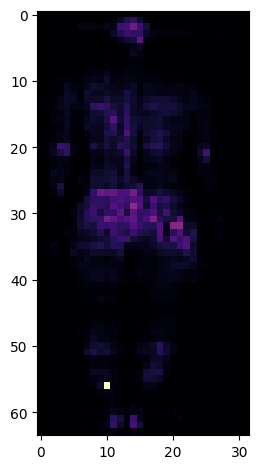
\includegraphics[width=\linewidth]{./EI_S1_F1.png}
      \caption{Exp. I, Sam. 1/F.45}
    \end{subfigure}
    \hfill
    \begin{subfigure}{0.3\textwidth}
      \centering
      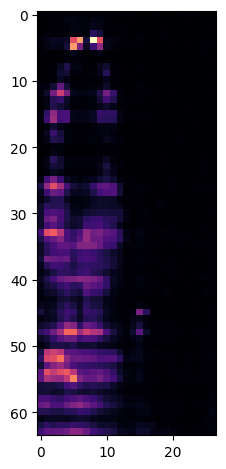
\includegraphics[width=\linewidth]{./EII_AirMat_B1.png}
      \caption{Exp. II, Sam. B1/AirMat}
    \end{subfigure}
    \hfill
    \begin{subfigure}{0.3\textwidth}
      \centering
      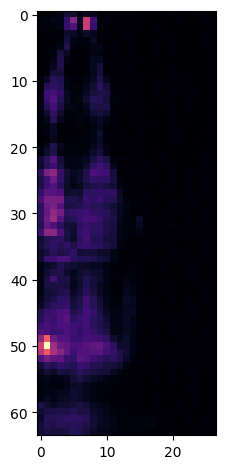
\includegraphics[width=\linewidth]{./EII_SpongeMat_B1.png}
      \caption{Exp. II, Sam. B1/SpongeMat}
    \end{subfigure}
  \end{figure}

  \subsection{Data Preprocessing}
  Two experimental versions were implemented:
  
  \subsubsection{First Version}
  \begin{enumerate}
    \item Data loading and description
    \item Data balancing by undersampling
    \item Feature extraction via LBP
    \item Model selection via Grid Search Cross Validation
    \item Performance evaluation
  \end{enumerate}

  \subsubsection{Second Version}
  \begin{enumerate}
    \item Data loading and description
    \item Data balancing by undersampling
    \item Data augmentation using pixel shifting (4px in x and y directions)
    \item Feature extraction via LBP
    \item Model selection via Grid Search Cross Validation
    \item Performance evaluation
  \end{enumerate}

  \subsection{Data Balancing and Augmentation}
  For balancing, undersampling was applied using the smallest class cardinality $N_{\min}$:
  
  \begin{equation*}
    \begin{aligned}
      \mathcal{C} &= \{ \mathcal{C}_1, \mathcal{C}_2, \ldots, \mathcal{C}_n \}\\
      N_{\min} &= \min_{\mathcal{C}_i \in \mathcal{C}} |\mathcal{C}_i|\\
      \mathcal{S} &= \bigcup_{\mathcal{C}_i \in \mathcal{C}} f(\mathcal{C}_i, N_{\min})
    \end{aligned}
  \end{equation*}
  
  For augmentation, non-destructive shifting was applied:
  
  \begin{equation*}
    \begin{aligned}
      \text{shift}&: \mathbb{R}^{m \times n} \times \mathbb{Z} \times \mathbb{Z} \to \mathbb{R}^{m \times n}\\
      M_{i+N_{\min}} &= \text{shift}(M_i, x, y)\\
      M_{i+N_{\min}+1} &= \text{shift}(M_i, -x, -y)
    \end{aligned}
  \end{equation*}

  \subsection{Feature Extraction}
  Local Binary Patterns (LBP) were computed for each sample:
  
  \begin{equation*}
    \begin{aligned}
      \text{LBP}_{P,R}(x_c, y_c) &= \sum_{p=0}^{P-1} 2^p \cdot s(g_p - g_c)
    \end{aligned}
  \end{equation*}

  \subsection{Model Selection}
  Grid Search Cross Validation (GSCV) was employed across four classifier blocks:
  
  \begin{enumerate}
    \item \textbf{Block 1: Tree-Based} - Decision Trees, Random Forest, KNN Coarse, AdaBoost
    \item \textbf{Block 2: KNN Variants} - KNN Fine, KNN Minkowski, KNN Weighted, KNN Medium
    \item \textbf{Block 3: Probabilistic} - Naïve Bayes, LDA, KNN Cosine
    \item \textbf{Block 4: SVM Variants} - Linear SVM, Quadratic SVM, Cubic SVM, Fifth SVM
  \end{enumerate}

  \section{Results}

  The full results are presented in Table \ref{tab:combined_results} for first version and in table \ref{tab:combined_results_aug} for second version.
  For the best model across all blocks, the performance metrics are presented in Table \ref{tab:best_results}.

  \begin{table}[ht!]
    \centering
    \caption{Performance Metrics Comparison Across All Blocks and Experiments (Non-Augmented Data)}
    \label{tab:combined_results}
    \resizebox{\textwidth}{!}{%
      \begin{tabular}{@{} l l l *{4}{S[table-format=1.4]} S[table-format=1.4] S[table-format=1.4] @{}}
        \toprule
        \textbf{Experiment} & \textbf{Block} & \textbf{Classifier} & \textbf{Accuracy} & \textbf{Precision} & \textbf{Recall} & \textbf{F1 Score} & \textbf{AUC Score} & \textbf{CV Score} \\
        \midrule

        \multirow{4}{*}{Experiment I} & Tree-Based & KNN Coarse & 0.8734 & 0.8733 & 0.8734 & 0.8733 & 0.9676 & 0.8639 \\
                                      & Tree-Based & Random Forest & 0.8359 & 0.8360 & 0.8359 & 0.8357 & 0.9512 & 0.8262 \\
                                      & Tree-Based & Decision Tree & 0.7928 & 0.7952 & 0.7928 & 0.7933 & 0.9081 & 0.7925 \\
                                      & Tree-Based & AdaBoost & 0.6605 & 0.6637 & 0.6605 & 0.6600 & 0.8020 & 0.6688 \\
                                      \cmidrule(lr){2-9}
                                      & KNN Variants & KNN Medium & 0.8734 & 0.8733 & 0.8734 & 0.8733 & 0.9676 & 0.8639 \\
                                      & KNN Variants & KNN Minkowski & 0.8688 & 0.8686 & 0.8688 & 0.8686 & 0.9673 & 0.8658 \\
                                      & KNN Variants & KNN Weighted & 0.8684 & 0.8685 & 0.8684 & 0.8684 & 0.9600 & 0.8652 \\
                                      & KNN Variants & KNN Fine & 0.8620 & 0.8633 & 0.8620 & 0.8623 & 0.9467 & 0.8643 \\
                                      \cmidrule(lr){2-9}
                                      & Probabilistic & KNN Cosine & 0.8146 & 0.8156 & 0.8146 & 0.8144 & 0.9439 & 0.8160 \\
                                      & Probabilistic & LDA & 0.5036 & 0.4962 & 0.5036 & 0.4879 & 0.7130 & 0.4912 \\
                                      & Probabilistic & Naive Bayes & 0.4429 & 0.4910 & 0.4429 & 0.4199 & 0.6637 & 0.4546 \\
                                      \cmidrule(lr){2-9}
                                      & SVM Variants & Quadratic SVM & 0.6555 & 0.6612 & 0.6555 & 0.6460 & {--} & 0.6540 \\
                                      & SVM Variants & Linear SVM & 0.5646 & 0.5795 & 0.5646 & 0.5504 & {--} & 0.5552 \\
                                      & SVM Variants & Cubic SVM & 0.5371 & 0.6224 & 0.5371 & 0.5243 & {--} & 0.5258 \\
                                      & SVM Variants & Fifth SVM & 0.4818 & 0.5765 & 0.4818 & 0.4593 & {--} & 0.4737 \\
                                      \midrule

        \multirow{4}{*}{Experiment II} & Tree-Based & Decision Tree & 0.5172 & 0.5157 & 0.5172 & 0.4937 & 0.6558 & 0.5391 \\
                                       & Tree-Based & Random Forest & 0.5172 & 0.5096 & 0.5172 & 0.5107 & 0.7646 & 0.5391 \\
                                       & Tree-Based & AdaBoost & 0.4483 & 0.4487 & 0.4483 & 0.4478 & 0.6766 & 0.5478 \\
                                       & Tree-Based & KNN Coarse & 0.4138 & 0.3867 & 0.4138 & 0.3878 & 0.6100 & 0.5043 \\
                                       \cmidrule(lr){2-9}
                                       & KNN Variants & KNN Fine & 0.5172 & 0.5640 & 0.5172 & 0.4875 & 0.6849 & 0.5304 \\
                                       & KNN Variants & KNN Medium & 0.4483 & 0.4454 & 0.4483 & 0.4301 & 0.6546 & 0.5043 \\
                                       & KNN Variants & KNN Weighted & 0.4483 & 0.4454 & 0.4483 & 0.4301 & 0.6546 & 0.5043 \\
                                       & KNN Variants & KNN Minkowski & 0.4483 & 0.4454 & 0.4483 & 0.4301 & 0.6546 & 0.5043 \\
                                       \cmidrule(lr){2-9}
                                       & Probabilistic & KNN Cosine & 0.5517 & 0.5552 & 0.5517 & 0.5526 & 0.7247 & 0.4609 \\
                                       & Probabilistic & Naive Bayes & 0.2759 & 0.2299 & 0.2759 & 0.2088 & 0.4215 & 0.4174 \\
                                       & Probabilistic & LDA & 0.2414 & 0.2324 & 0.2414 & 0.2358 & 0.4465 & 0.4348 \\
                                       \cmidrule(lr){2-9}
                                       & SVM Variants & Linear SVM & 0.5517 & 0.5699 & 0.5517 & 0.5507 & {--} & 0.4348 \\
                                       & SVM Variants & Quadratic SVM & 0.4483 & 0.4650 & 0.4483 & 0.4536 & {--} & 0.4609 \\
                                       & SVM Variants & Cubic SVM & 0.3793 & 0.3994 & 0.3793 & 0.2920 & {--} & 0.4435 \\
                                       & SVM Variants & Fifth SVM & 0.3793 & 0.4185 & 0.3793 & 0.3208 & {--} & 0.4522 \\
                                       \bottomrule
      \end{tabular}
    }

    \vspace{0.2cm}
    \small
    Note: -- indicates that the metric was not available for that model.
  \end{table}

  
  \begin{table}[ht!]
    \centering
    \caption{Performance Metrics Comparison Across All Experiments and Blocks}
    \label{tab:combined_results_aug}
    \resizebox{\textwidth}{!}{%
      \begin{tabular}{@{} l l l *{4}{S[table-format=1.4]} S[table-format=1.4] S[table-format=1.4] @{}}
        \toprule
        \textbf{Experiment} & \textbf{Block} & \textbf{Classifier} & \textbf{Accuracy} & \textbf{Precision} & \textbf{Recall} & \textbf{F1 Score} & \textbf{AUC Score} & \textbf{CV Score} \\
        \midrule

        \multirow{12}{*}{Experiment I} & \multirow{4}{*}{Tree-Based} & KNN Coarse & 0.8734 & 0.8733 & 0.8734 & 0.8733 & 0.9676 & 0.8639 \\
                                       &                             & Random Forest & 0.8359 & 0.8360 & 0.8359 & 0.8357 & 0.9512 & 0.8262 \\
                                       &                             & Decision Tree & 0.7928 & 0.7952 & 0.7928 & 0.7933 & 0.9081 & 0.7925 \\
                                       &                             & AdaBoost & 0.6605 & 0.6637 & 0.6605 & 0.6600 & 0.8020 & 0.6688 \\
                                       \cmidrule(lr){2-9}
                                       & \multirow{4}{*}{KNN Variants} & KNN Medium & 0.8734 & 0.8733 & 0.8734 & 0.8733 & 0.9676 & 0.8639 \\
                                       &                             & KNN Minkowski & 0.8688 & 0.8686 & 0.8688 & 0.8686 & 0.9673 & 0.8658 \\
                                       &                             & KNN Weighted & 0.8684 & 极 0.8685 & 0.8684 & 0.8684 & 0.9600 & 0.8652 \\
                                       &                             & KNN Fine & 0.8620 & 0.8633 & 0.8620 & 0.8623 & 极 0.9467 & 0.8643 \\
                                       \cmidrule(lr){2-9}
                                       & \multirow{3}{*}{Probabilistic} & KNN Cosine & 0.8142 & 0.8154 & 0.8142 & 0.8140 & 0.9438 & 0.8160 \\
                                       &                             & LDA & 0.5036 & 0.4962 & 0.5036 & 0.4879 & 0.7130 & 0.4912 \\
                                       &                             & Naive Bayes & 0.4429 & 0.4910 & 0.4429 & 0.4199 & 0.6637 & 0.4546 \\
                                       \cmidrule(lr){2-9}
                                       & \multirow{4}{*}{SVM Variants} & Quadratic SVM & 0.6555 & 0.6612 & 0.6555 & 0.6460 & {--} & 0.6540 \\
                                       &                             & Linear SVM & 0.5646 & 0.5793 & 0.5646 & 0.5504 & {--} & 0.5551 \\
                                       &                             & Cubic SVM & 0.5371 & 0.6224 & 0.5371 & 0.5243 & {--} & 0.5260 \\
                                       &                             & Fifth SVM & 0.4818 & 0.5765 & 0.4818 & 0.4592 & {--} & 0.4737 \\
                                       \midrule

        \multirow{15}{*}{Experiment II} & \multirow{4}{*}{Tree-Based} & Decision Tree & 0.5172 & 0.5157 & 0.5172 & 0.4937 & 0.6558 & 0.5391 \\
                                        &                             & Random Forest & 0.5172 & 0.5096 & 0.5172 & 0.5107 & 0.7646 & 0.5391 \\
                                        &                             & AdaBoost & 0.4483 & 0.4487 & 0.4483 & 0.4478 & 0.6766 & 0.5478 \\
                                        &                             & KNN Coarse & 0.4138 & 0.3867 & 0.4138 & 0.3878 & 0.6100 & 0.5043 \\
                                        \cmidrule(lr){2-9}
                                        & \multirow{4}{*}{KNN Variants} & KNN Fine & 0.5172 & 0.5640 & 0.5172 & 0.4875 & 0.6849 & 0.5304 \\
                                        &                             & KNN Medium & 0.4483 & 0.4454 & 0.4483 & 0.4301 & 0.6546 & 0.5043 \\
                                        &                             & KNN Weighted & 0.4483 & 0.4454 & 0.4483 & 0.4301 & 0.6546 & 0.5043 \\
                                        &                             & KNN Minkowski & 0.4483 & 0.4454 & 0.4483 & 0.4301 & 0.6546 & 0.5043 \\
                                        \cmidrule(lr){2-9}
                                        & \multirow{3}{*}{Probabilistic} & KNN Cosine & 0.5517 & 0.5552 & 0.5517 & 0.5526 & 0.7247 & 0.4609 \\
                                        &                             & Naive Bayes & 0.2759 & 0.2299 & 0.2759 & 0.2088 & 0.4215 & 0.4174 \\
                                        &                             & LDA & 0.2414 & 0.2324 & 0.2414 & 0.2358 & 0.4465 & 0.4348 \\
                                        \cmidrule(lr){2-9}
                                        & \multirow{4}{*}{SVM Variants} & Linear SVM & 0.5517 & 0.5699 & 0.5517 & 0.5507 & {--} & 0.4348 \\
                                        &                             & Quadratic SVM & 0.4483 & 0.4650 & 0.4483 & 0.4536 & {--} & 0.4609 \\
                                        &                             & Cubic SVM & 0.3793 & 0.3994 & 0.3793 & 0.2920 & {--} & 0.4435 \\
                                        &                             & Fifth SVM & 0.3793 & 0.4185 & 0.3793 & 0.3208 & {--} & 0.4522 \\
                                        \bottomrule
      \end{tabular}
    }

  \vspace{0.2cm}
  \small
  Note: -- indicates that the metric was not available for that model.
  \end{table}


  \begin{table}[!ht]
    \caption{Best performance metrics across all blocks and experiments}
    \label{tab:best_results}
    \centering
    \scriptsize
    \begin{tabular}{@{} l l *{5}{S[table-format=1.3]} S[table-format=1.4] S[table-format=1.3] @{}}
      \toprule
      \multirow{2}{*}{\textbf{Experiment}} & \multirow{2}{*}{\textbf{Best Model}} & \textbf{Acc.} & \textbf{Prec.} & \textbf{Rec.} & \textbf{F1} & \textbf{AUC} & \textbf{CV} \\
       & & & & & & \textbf{Score} & \textbf{Score} \\
      \midrule
      \multicolumn{8}{l}{\textbf{Experiment I}} \\
      \midrule
      Block 1: Tree-Based & KNN Coarse & 0.8734 & 0.8733 & 0.8734 & 0.8733 & 0.9676 & 0.8639 \\
      Block 2: KNN Variants & KNN Medium & 0.8734 & 0.8733 & 0.8734 & 0.8733 & 0.9676 & 0.8639 \\
      Block 3: Probabilistic & KNN Cosine & 0.8146 & 0.8156 & 0.8146 & 0.8144 & 0.9439 & 0.8160 \\
      Block 4: SVM Variants & Quadratic SVM & 0.6555 & 0.6612 & 0.6555 & 0.6460 & {N/A} & 0.6540 \\
      \midrule
      \multicolumn{8}{l}{\textbf{Experiment II}} \\
      \midrule
      Block 1: Tree-Based & Decision Tree & 0.5172 & 0.5157 & 0.5172 & 0.4937 & 0.6558 & 0.5391 \\
      Block 2: KNN Variants & KNN Fine & 0.5172 & 0.5640 & 0.5172 & 0.4875 & 0.6849 & 0.5304 \\
      Block 3: Probabilistic & KNN Cosine & 0.5517 & 0.5552 & 0.5517 & 0.5526 & 0.7247 & 0.4609 \\
      Block 4: SVM Variants & Linear SVM & 0.5517 & 0.5699 & 0.5517 & 0.5507 & {N/A} & 0.4348 \\
      \bottomrule
    \end{tabular}
  \end{table}

  \begin{table}[!ht]
    \caption{Impact of data augmentation on model performance}
    \label{tab:augmentation}
    \centering
    \scriptsize
    \begin{tabular}{@{} l l *{5}{S[table-format=1.3]} S[table-format=1.4] S[table-format=1.3] @{}}
      \toprule
      \multirow{2}{*}{\textbf{Experiment}} & \multirow{2}{*}{\textbf{Best Model}} & \textbf{Acc.} & \textbf{Prec.} & \textbf{Rec.} & \textbf{F1} & \textbf{AUC} & \textbf{CV} \\
       & & & & & & \textbf{Score} & \textbf{Score} \\
      \midrule
      \multicolumn{8}{l}{\textbf{Without Data Augmentation (Experiment I)}} \\
      \midrule
      Tree-Based & KNN Coarse & 0.873 & 0.873 & 0.873 & 0.873 & 0.968 & 0.864 \\
      KNN Variants & KNN Medium & 0.873 & 0.873 & 0.873 & 0.873 & 0.968 & 0.864 \\
      Probabilistic & KNN Cosine & 0.814 & 0.815 & 0.814 & 0.814 & 0.944 & 0.816 \\
      SVM Variants & Quadratic SVM & 0.655 & 0.661 & 0.655 & 0.646 & {N/A} & 0.654 \\
      \midrule
      \multicolumn{8}{l}{\textbf{With Data Augmentation (Experiment II)}} \\
      \midrule
      Tree-Based & Decision Tree & 0.517 & 0.516 & 0.517 & 0.494 & 0.656 & 0.539 \\
      KNN Variants & KNN Fine & 0.517 & 0.564 & 0.517 & 0.487 & 0.685 & 0.530 \\
      Probabilistic & KNN Cosine & 0.552 & 0.555 & 0.552 & 0.553 & 0.725 & 0.461 \\
      SVM Variants & Linear SVM & 0.552 & 0.570 & 0.552 & 0.551 & {N/A} & 0.435 \\
      \bottomrule
    \end{tabular}
  \end{table}

    % ==================== EXPERIMENT I PLOTS ====================
% Block 1: Tree-Based (Experiment I)
    \begin{figure}[!ht]
        \begin{subfigure}{0.33\textwidth}
            \centering
            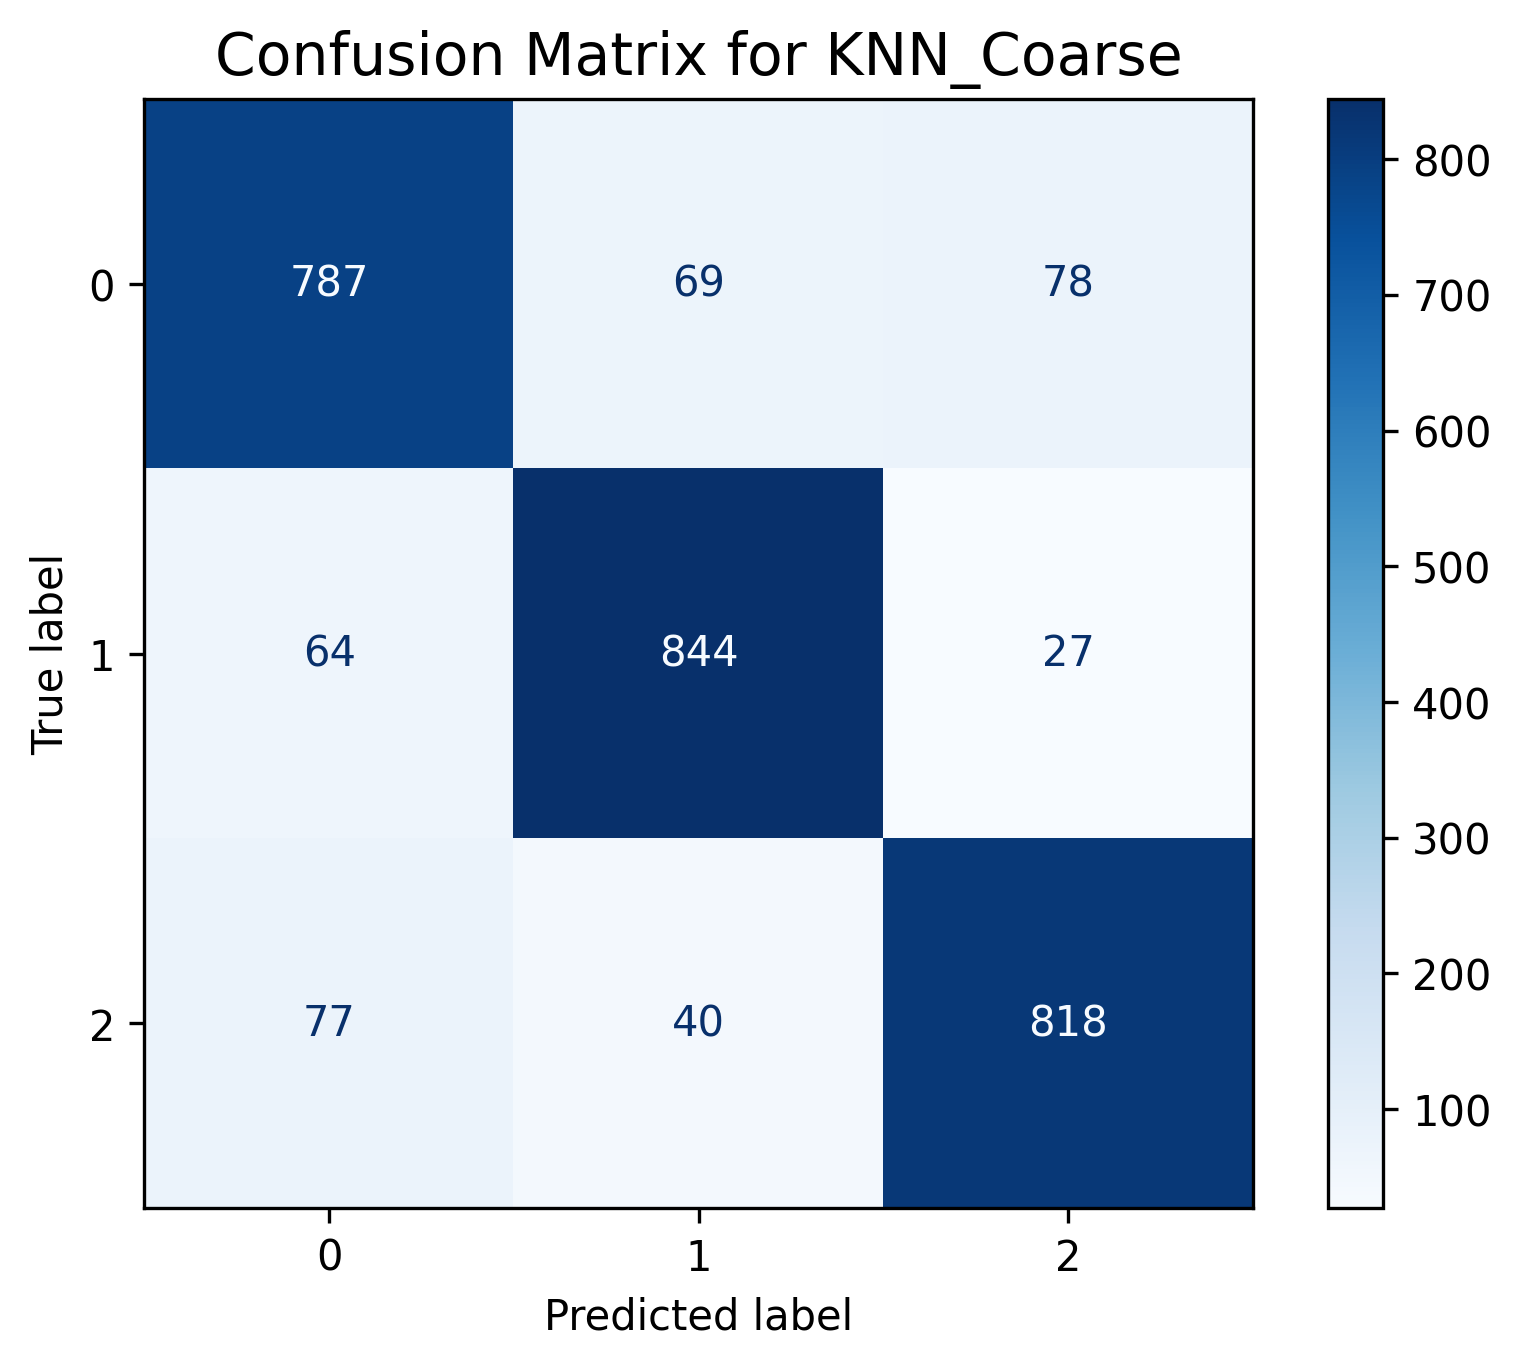
\includegraphics[width=\textwidth]{code/ResultsMainAugZip/plots/Block1_Tree_Based_Experiment_I/confusion_matrix_KNN_Coarse.png}
            \caption{Confusion Matrix}
        \end{subfigure}
        \begin{subfigure}{0.33\textwidth}
            \centering
            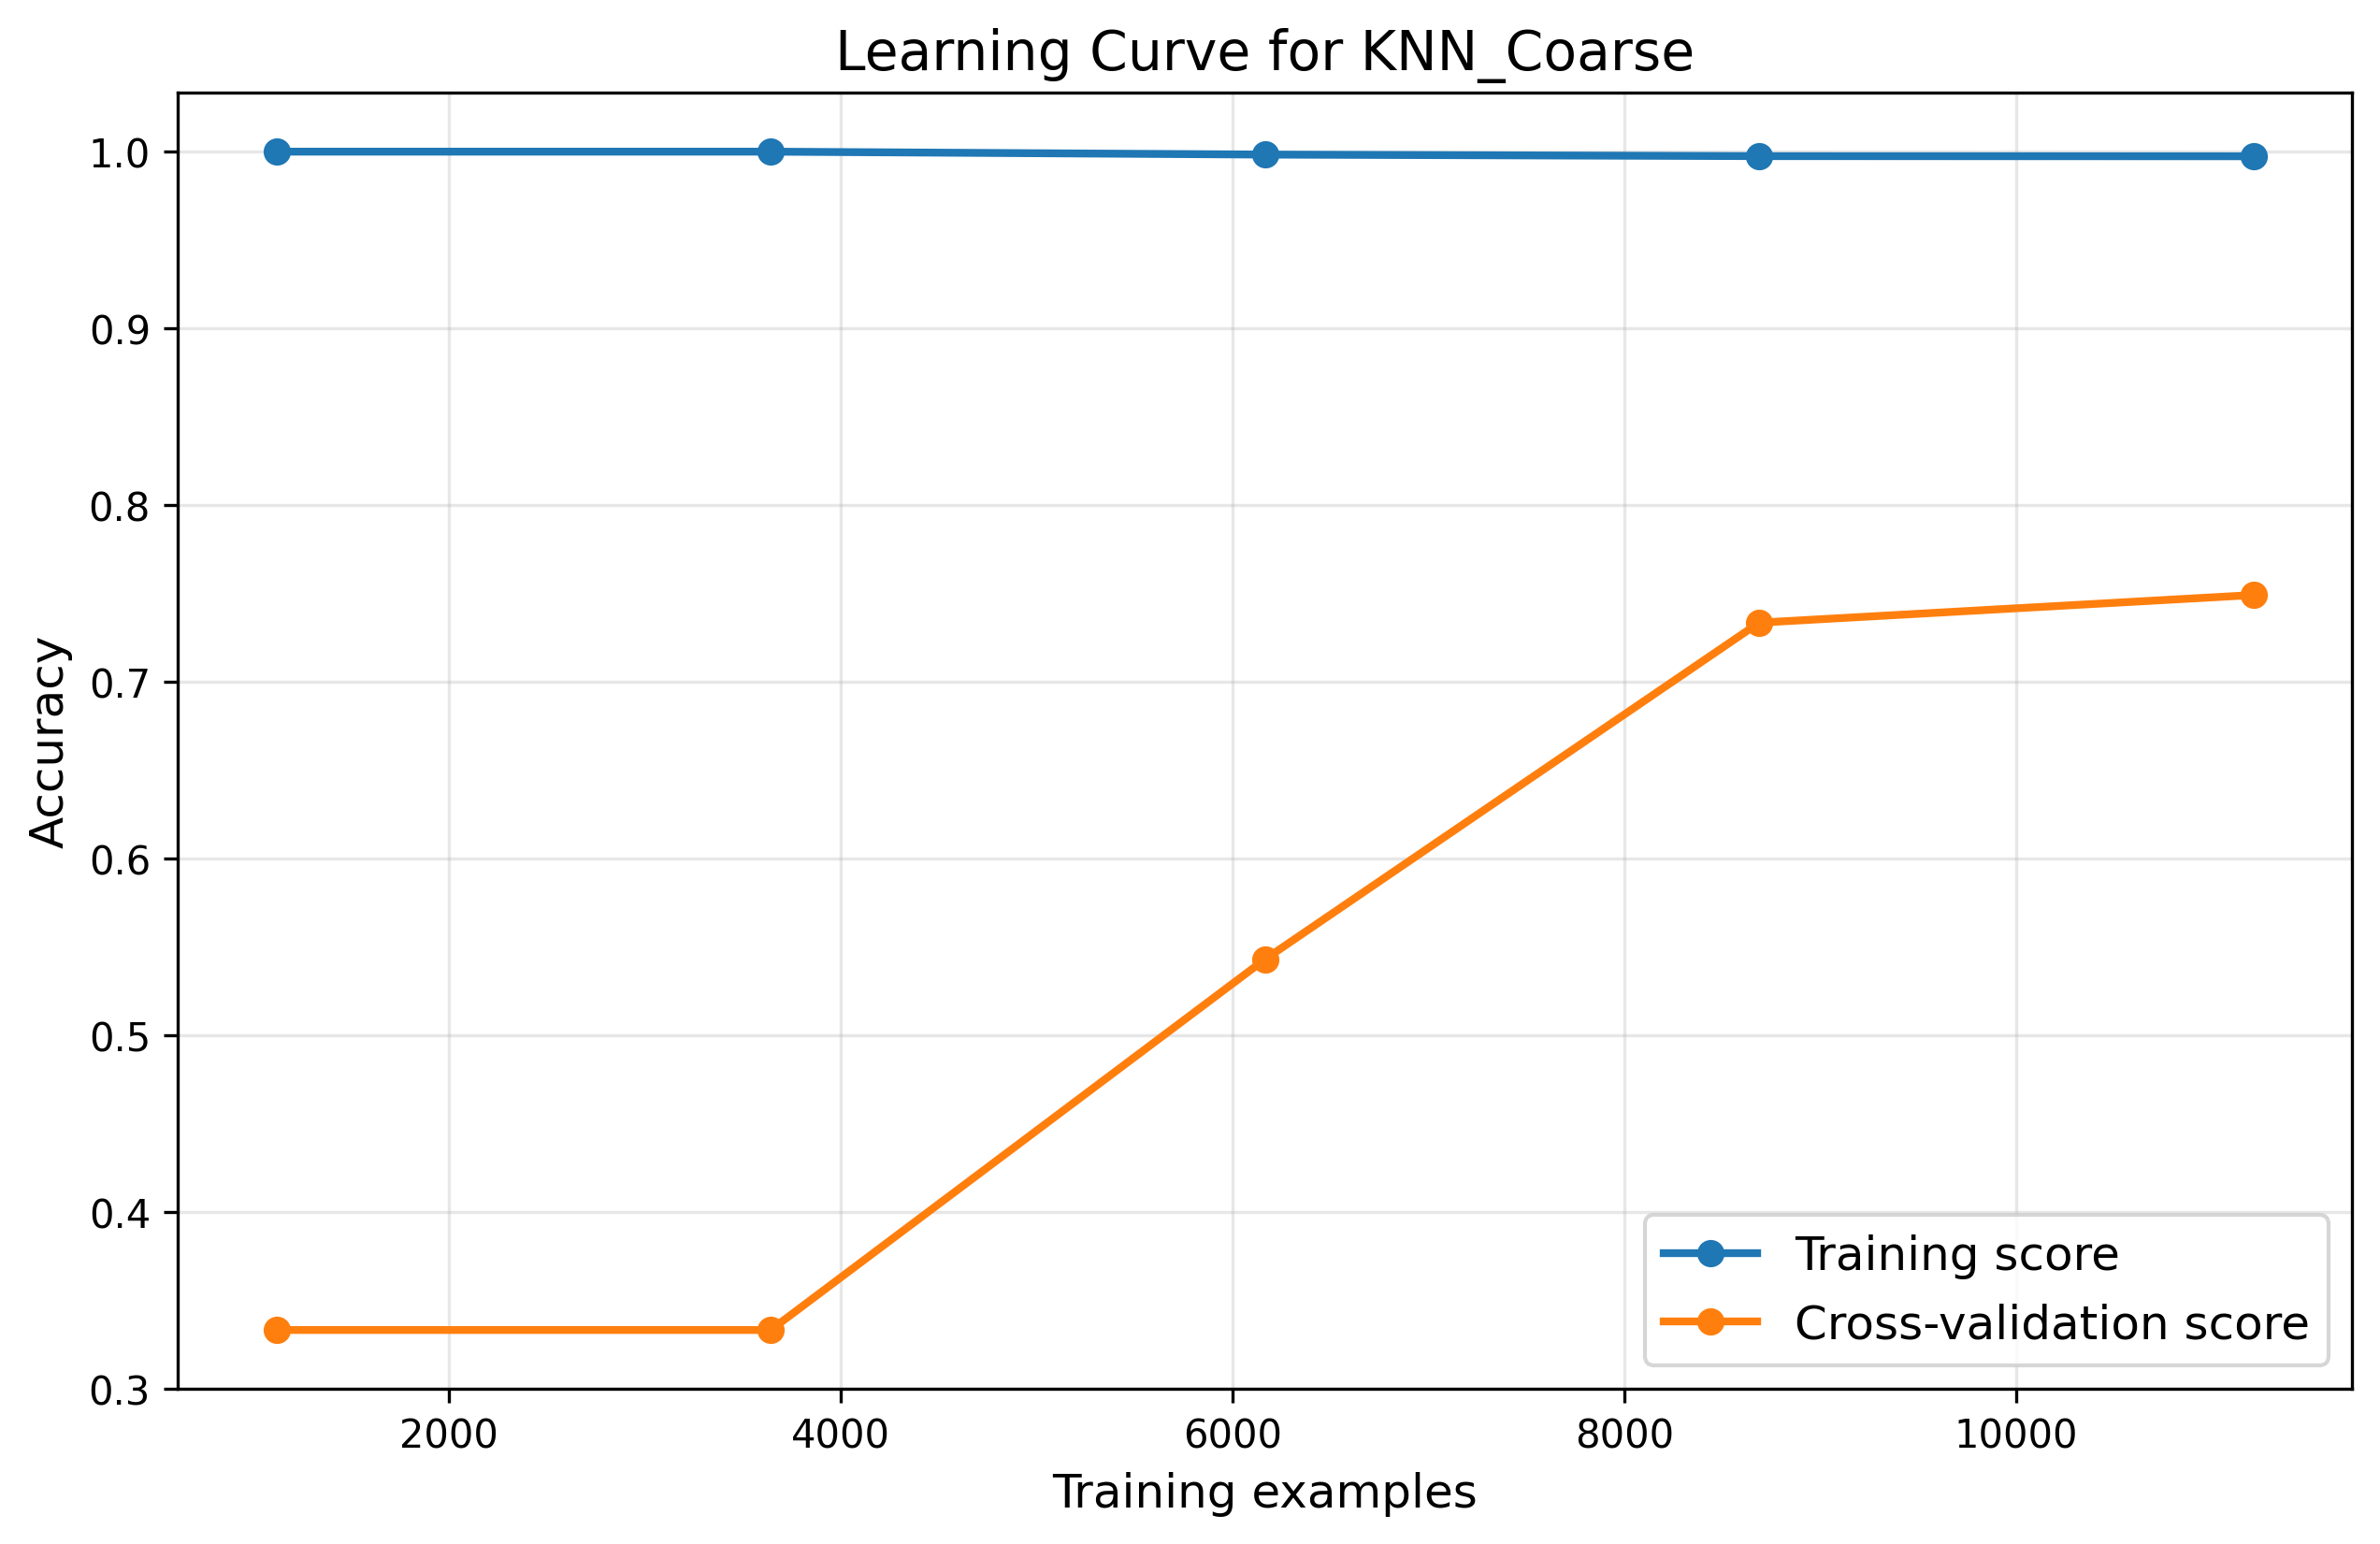
\includegraphics[width=\textwidth]{code/ResultsMainAugZip/plots/Block1_Tree_Based_Experiment_I/learning_curve_KNN_Coarse.png}
            \caption{Learning Curve}
        \end{subfigure}
        \begin{subfigure}{0.33\textwidth}
            \centering
            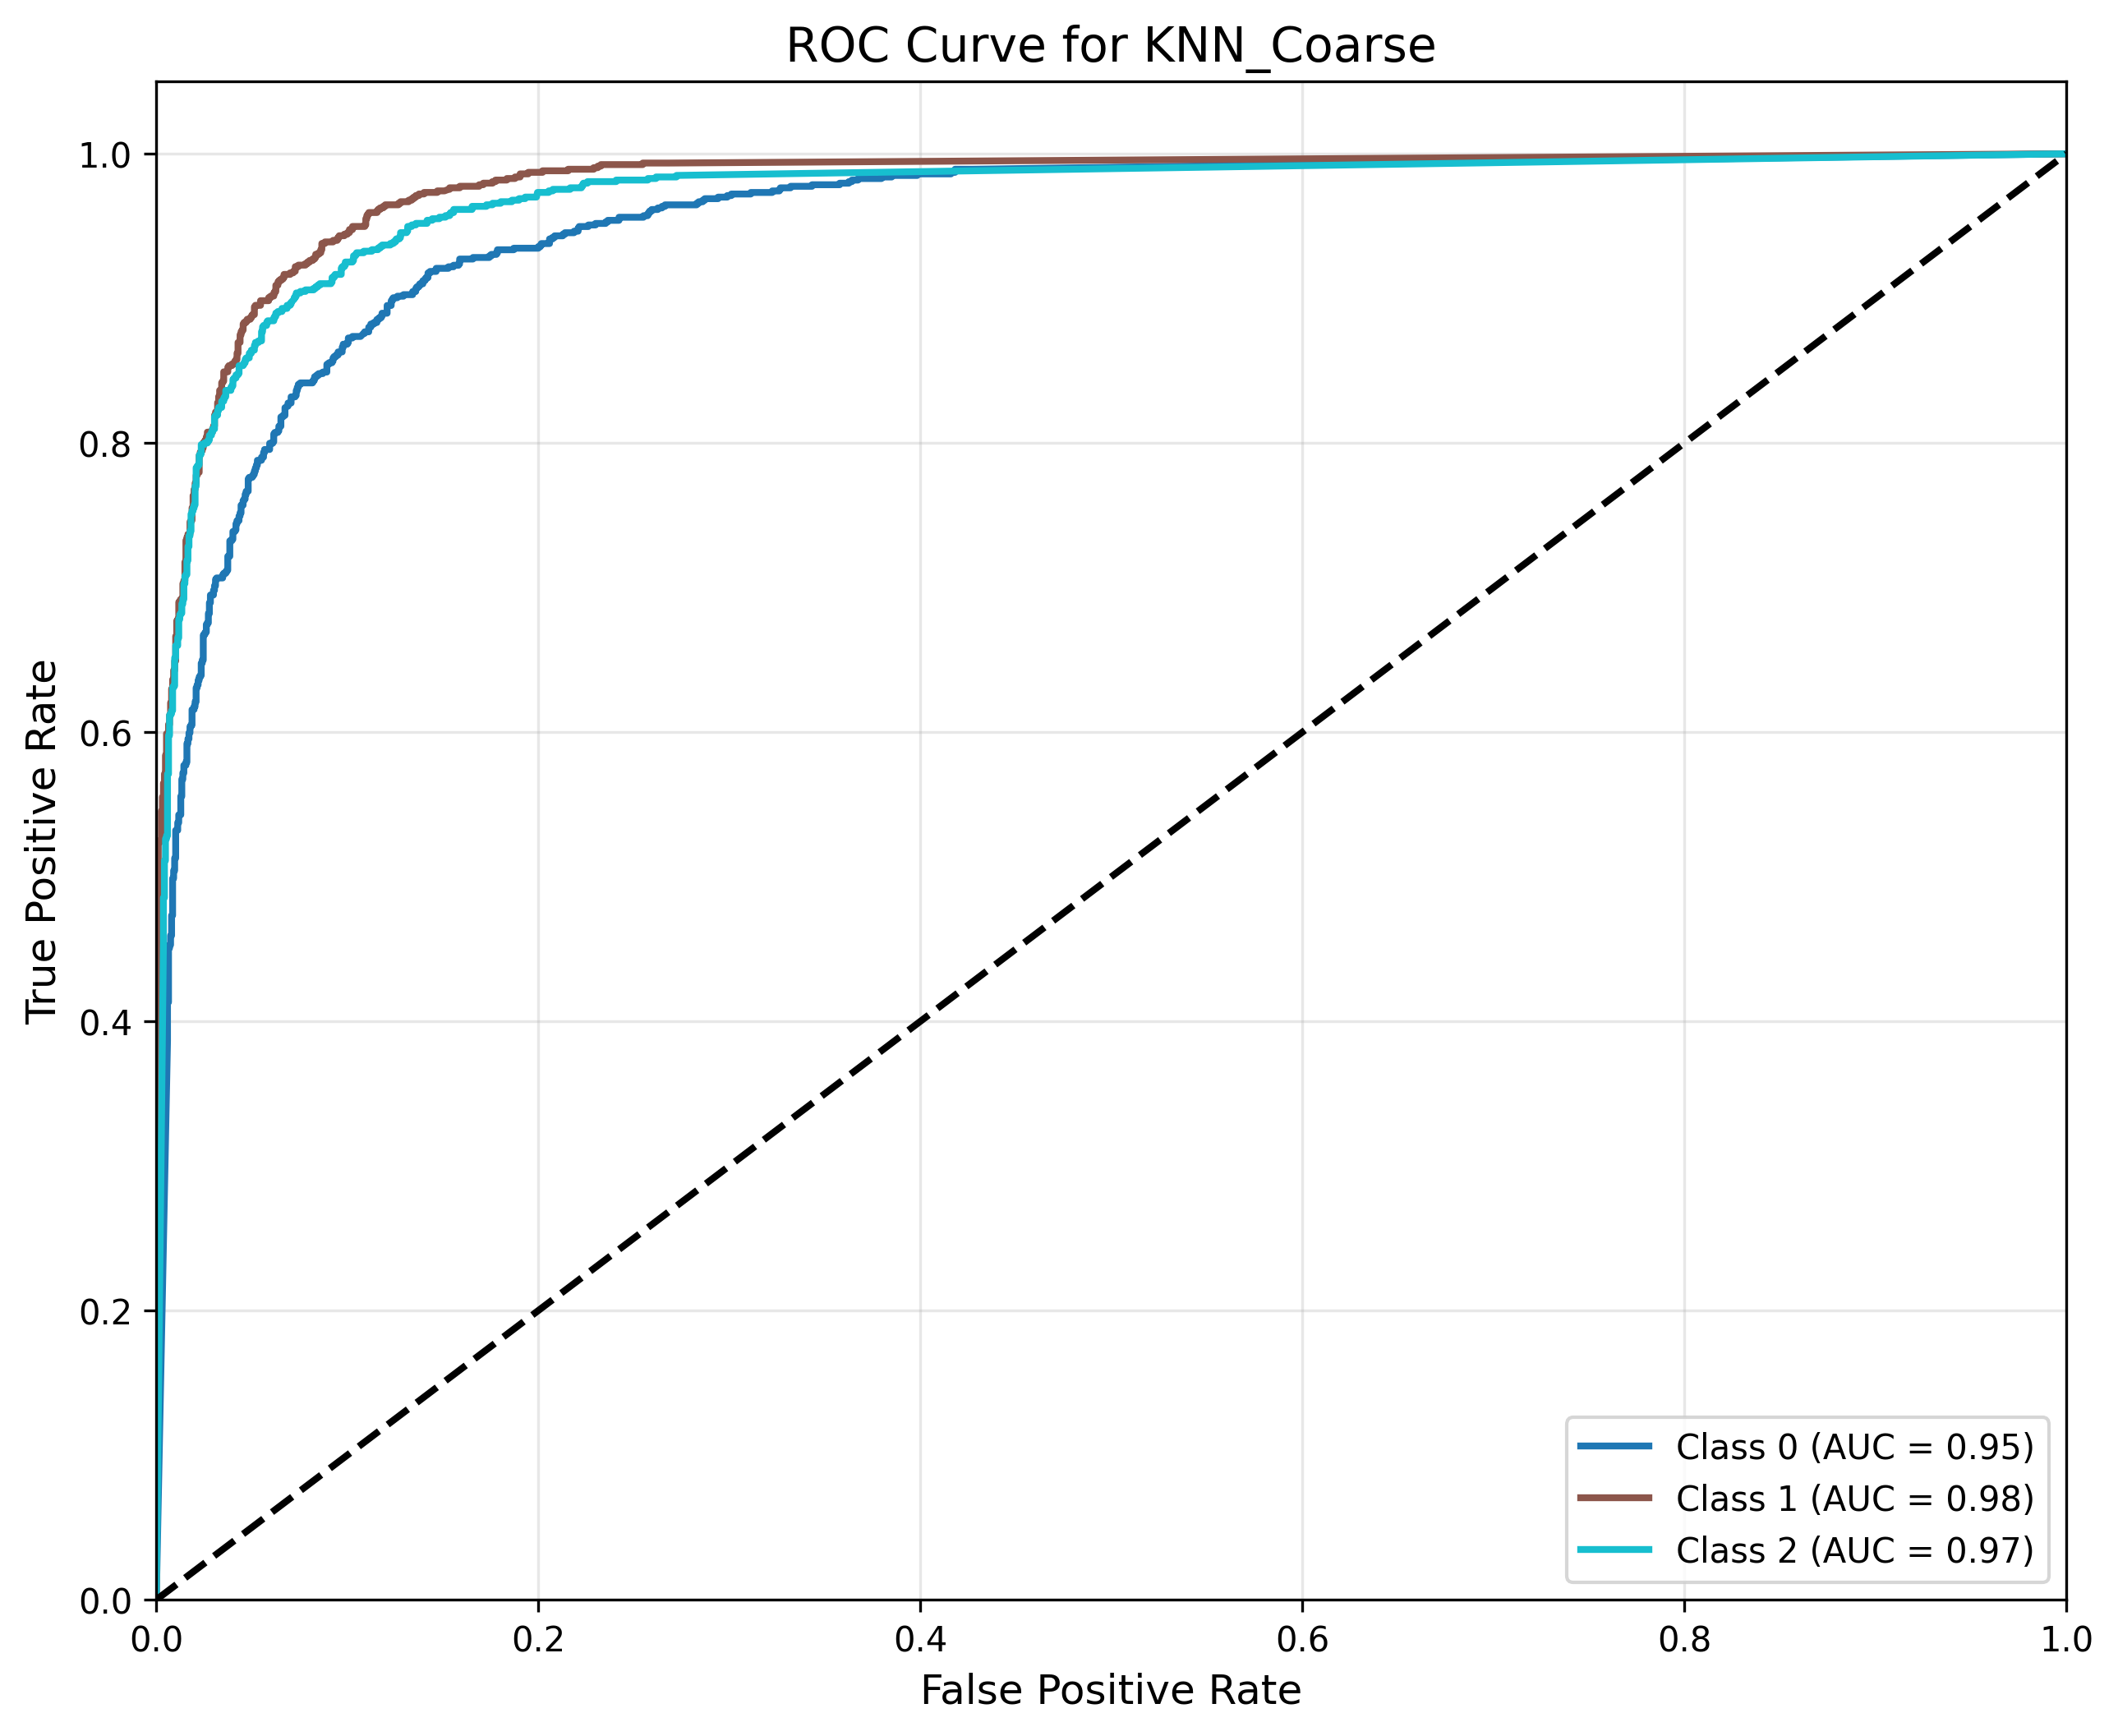
\includegraphics[width=\textwidth]{code/ResultsMainAugZip/plots/Block1_Tree_Based_Experiment_I/roc_curve_KNN_Coarse.png}
            \caption{ROC Curve}
        \end{subfigure}
    \end{figure}
    
    % Block 2: KNN Variants (Experiment I)
    \begin{figure}[!ht]
        \begin{subfigure}{0.33\textwidth}
            \centering
            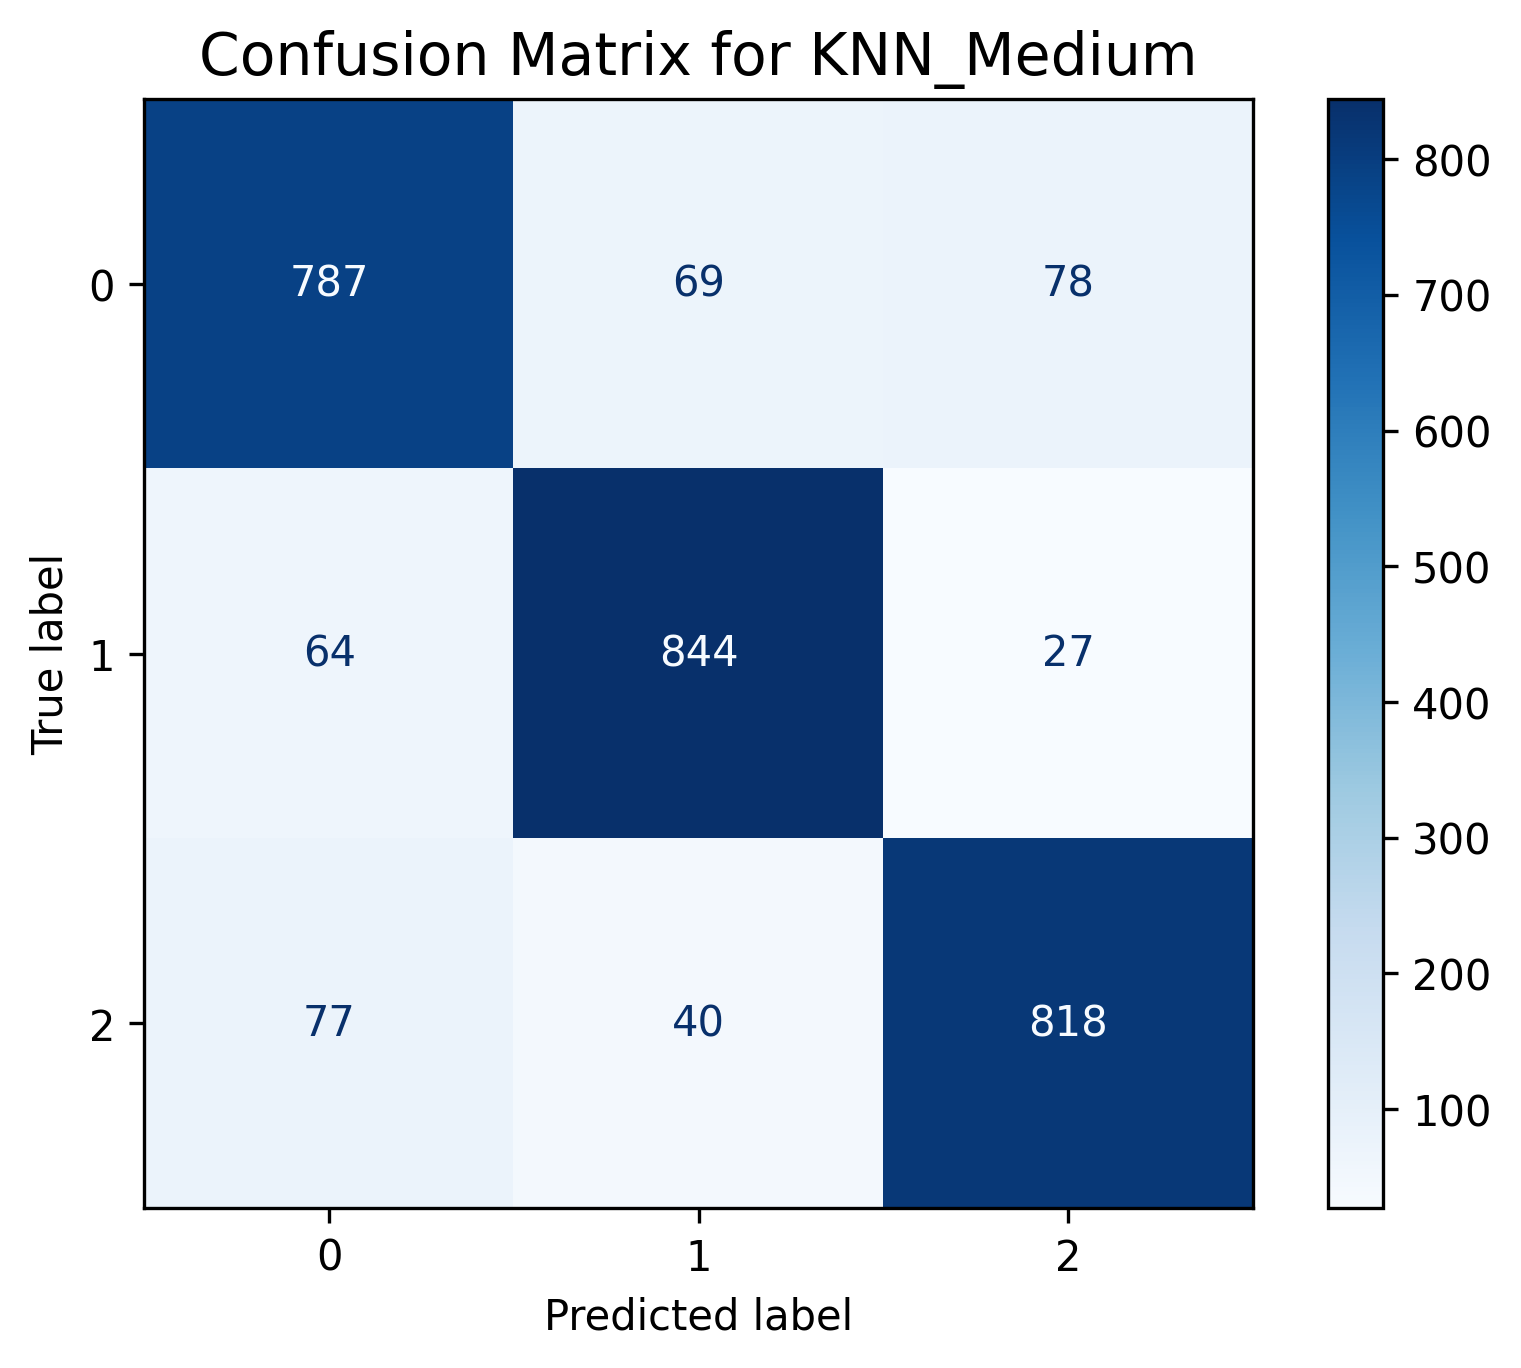
\includegraphics[width=\textwidth]{code/ResultsMainAugZip/plots/Block2_KNN_Variants_Experiment_I/confusion_matrix_KNN_Medium.png}
            \caption{Confusion Matrix}
        \end{subfigure}
        \begin{subfigure}{0.33\textwidth}
            \centering
            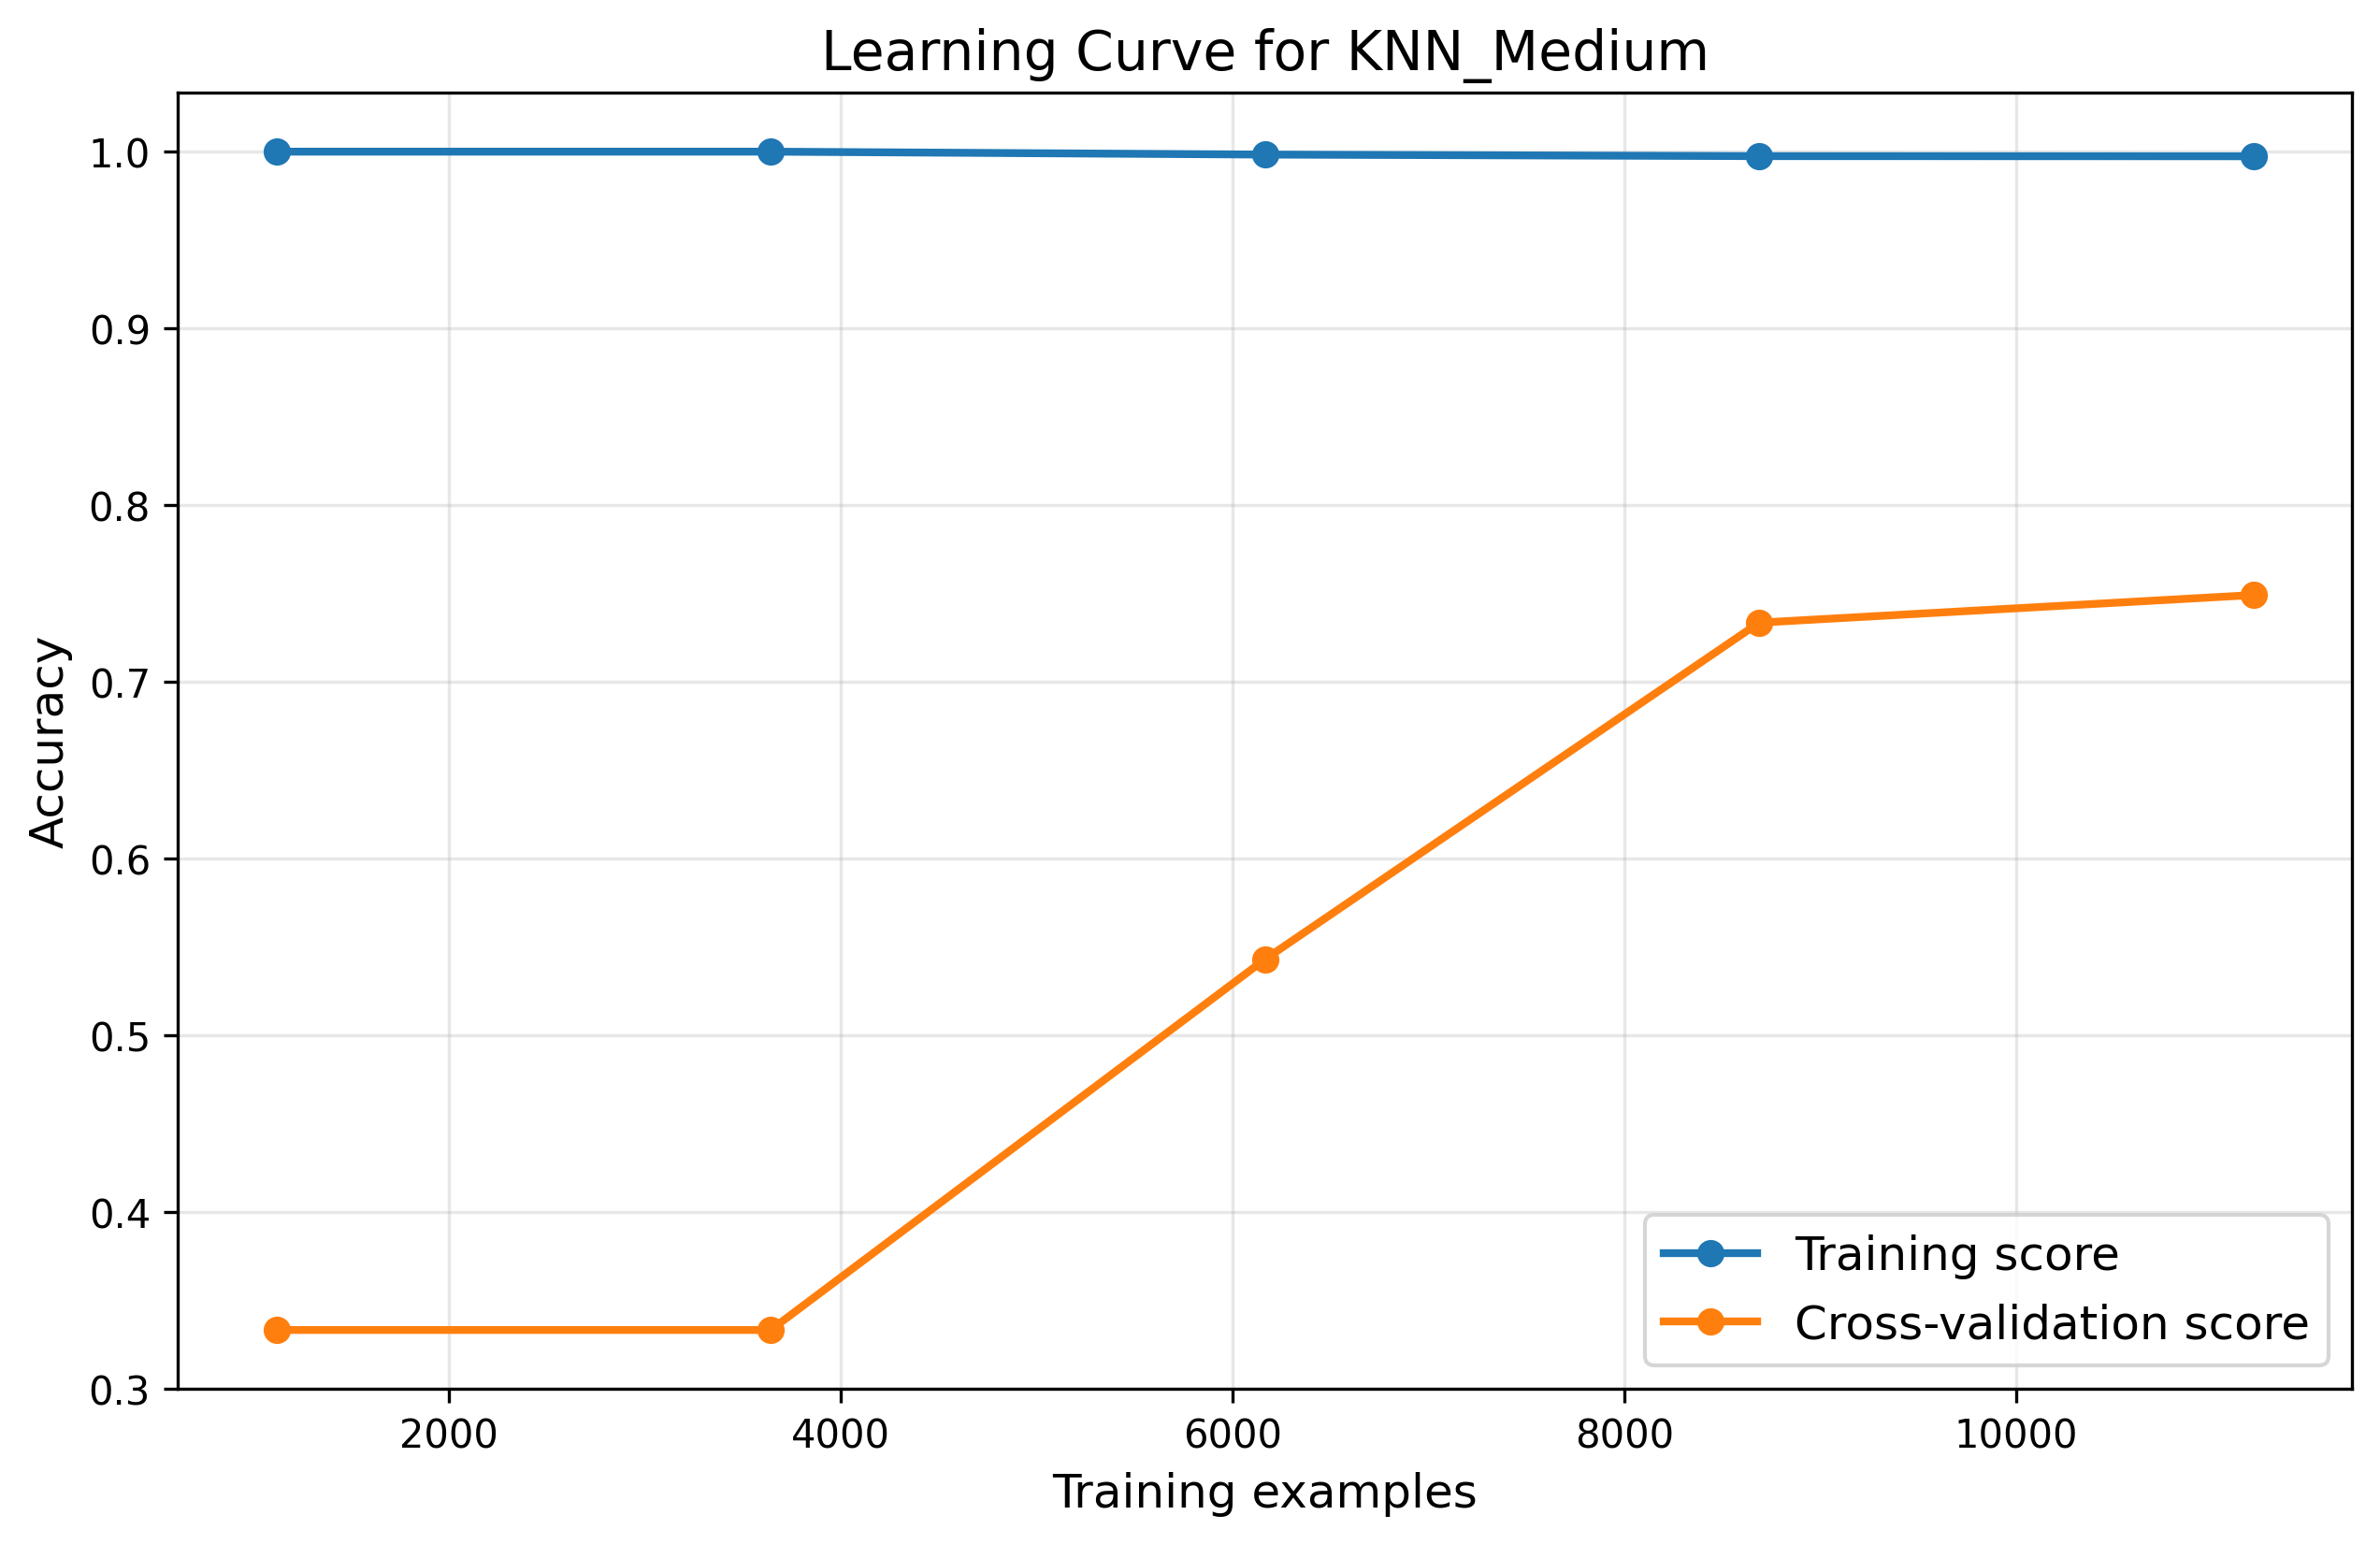
\includegraphics[width=\textwidth]{code/ResultsMainAugZip/plots/Block2_KNN_Variants_Experiment_I/learning_curve_KNN_Medium.png}
            \caption{Learning Curve}
        \end{subfigure}
        \begin{subfigure}{0.33\textwidth}
            \centering
            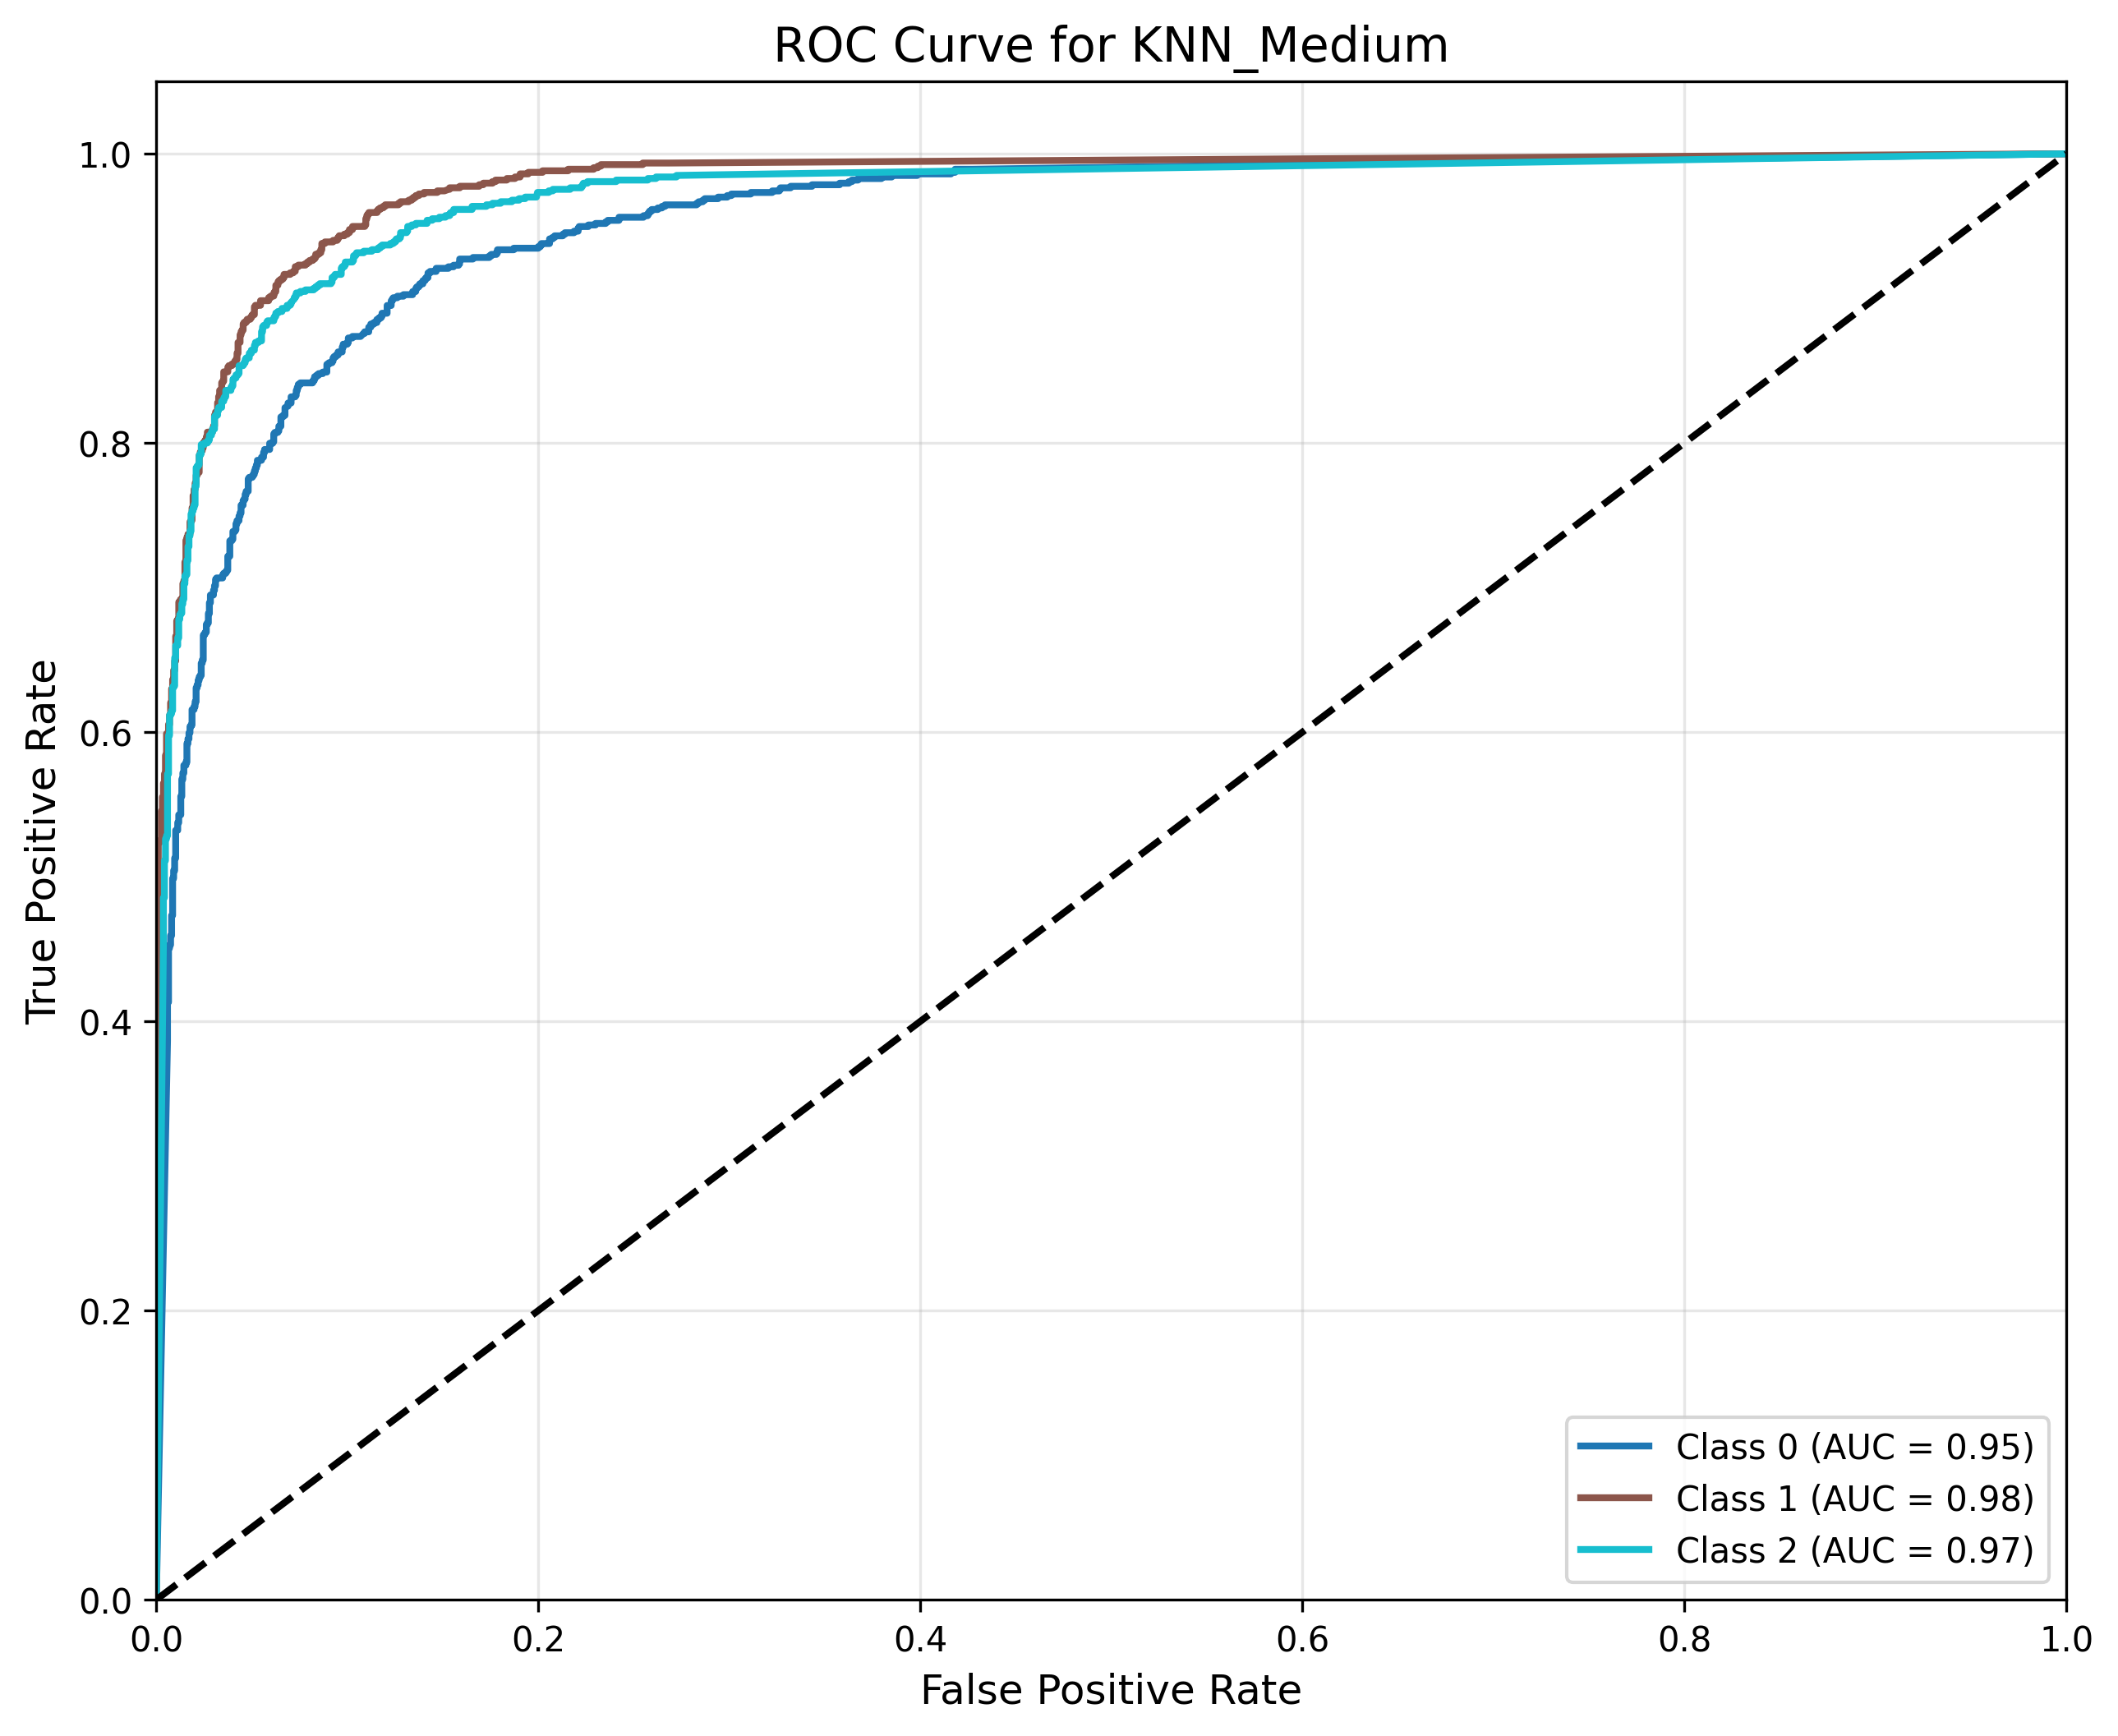
\includegraphics[width=\textwidth]{code/ResultsMainAugZip/plots/Block2_KNN_Variants_Experiment_I/roc_curve_KNN_Medium.png}
            \caption{ROC Curve}
        \end{subfigure}
    \end{figure}
    
    % Block 3: Probabilistic (Experiment I)
    \begin{figure}[!ht]
        \begin{subfigure}{0.33\textwidth}
            \centering
            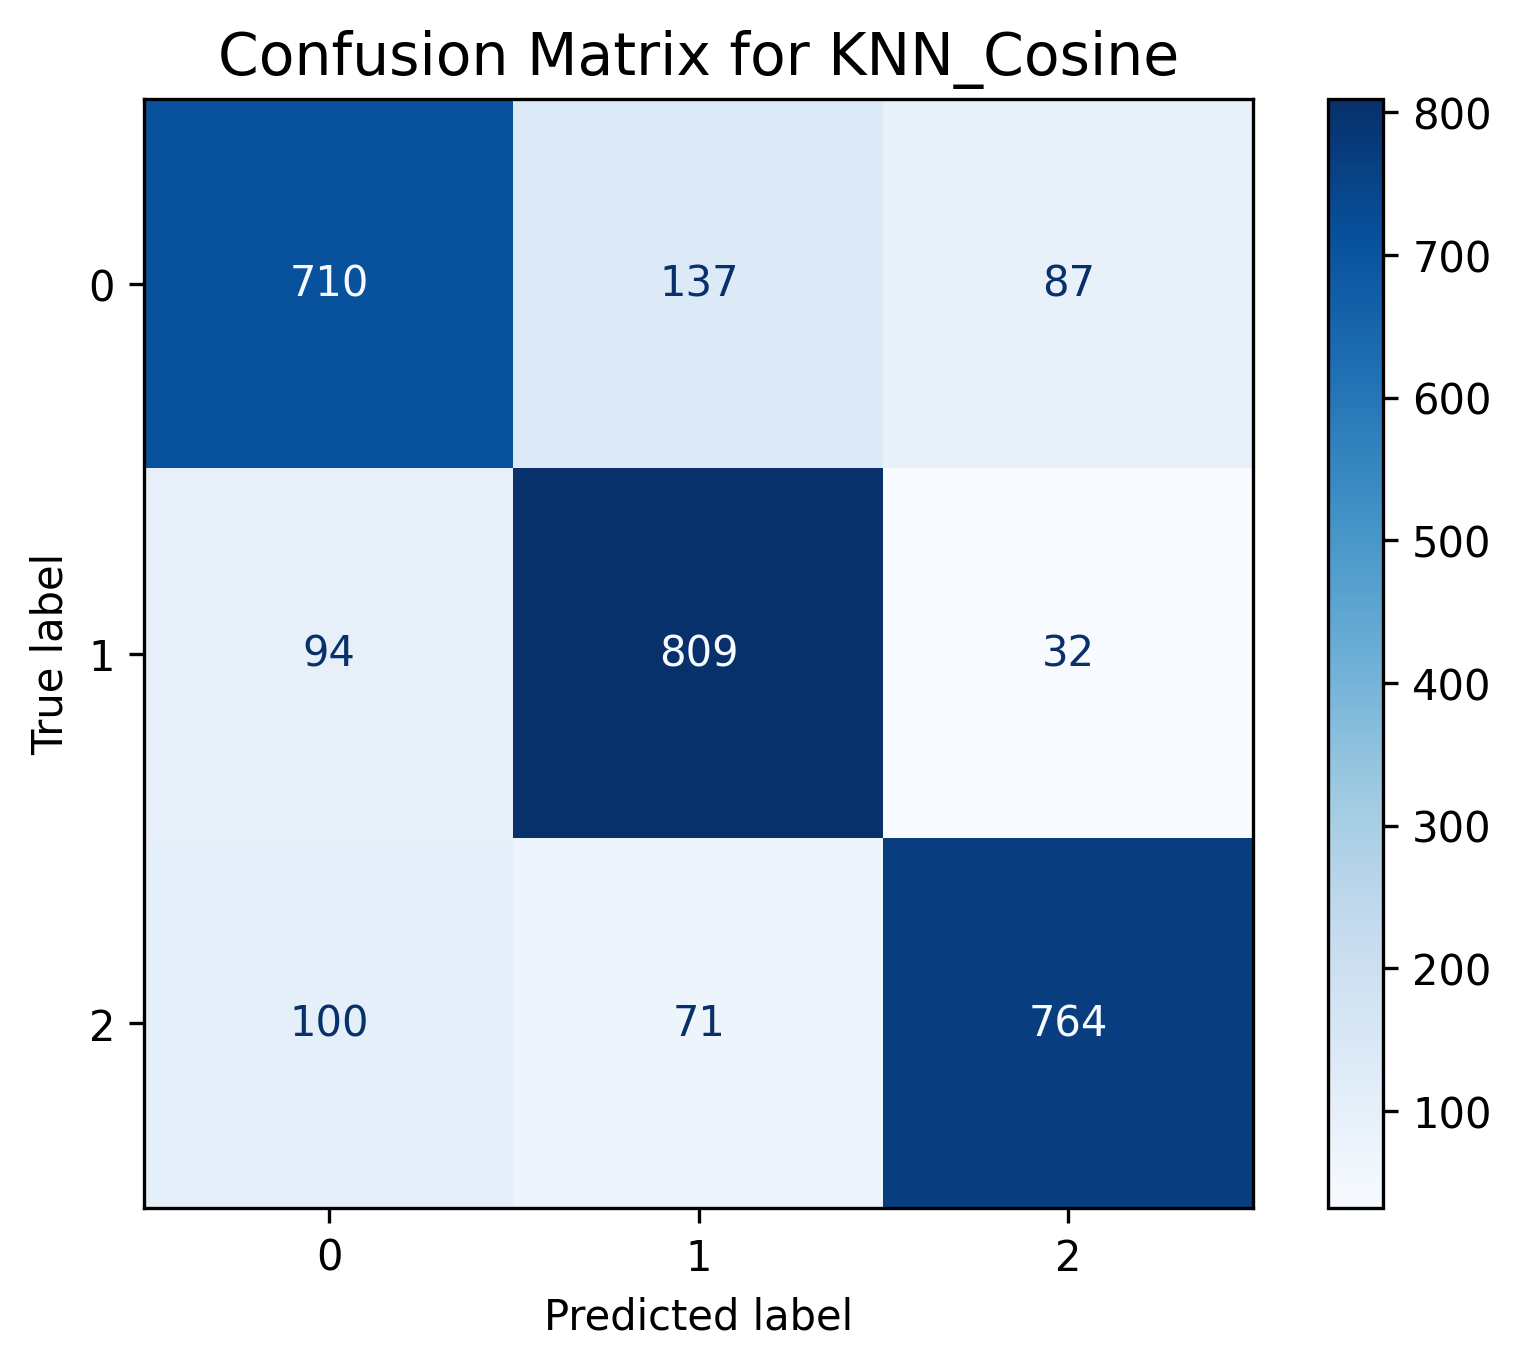
\includegraphics[width=\textwidth]{code/ResultsMainAugZip/plots/Block3_Probabilistic_Experiment_I/confusion_matrix_KNN_Cosine.png}
            \caption{Confusion Matrix}
        \end{subfigure}
        \begin{subfigure}{0.33\textwidth}
            \centering
            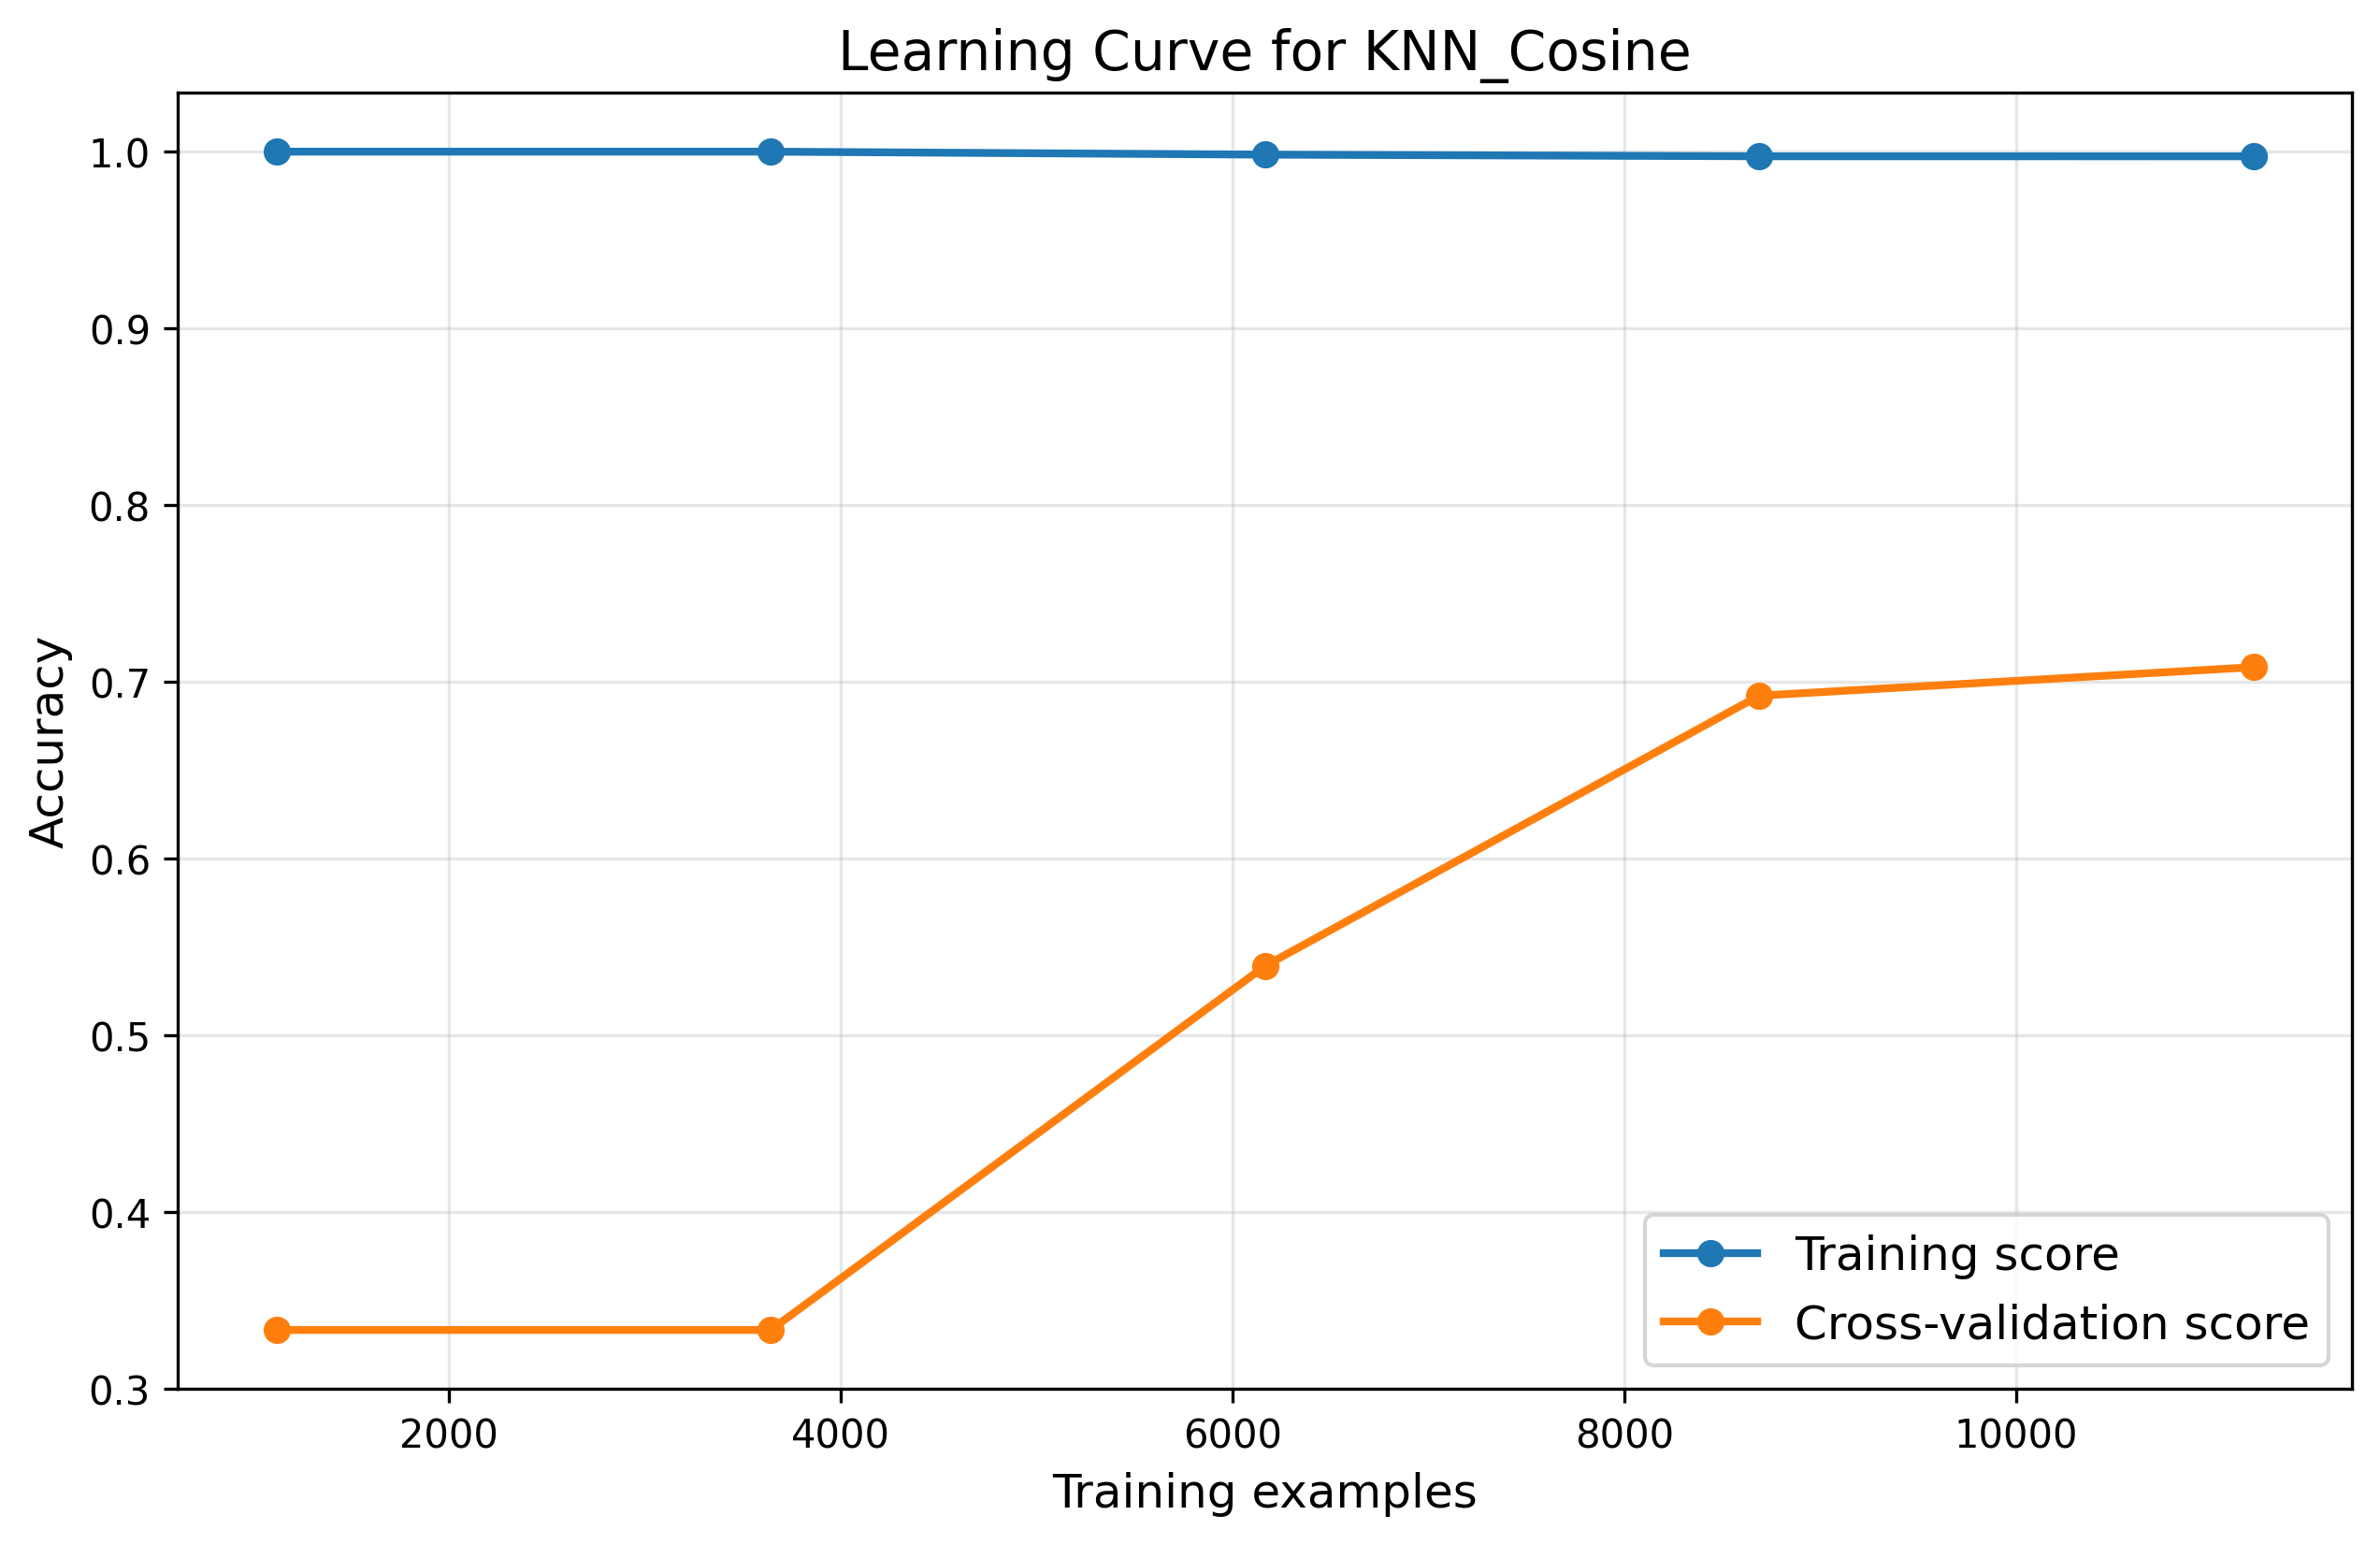
\includegraphics[width=\textwidth]{code/ResultsMainAugZip/plots/Block3_Probabilistic_Experiment_I/learning_curve_KNN_Cosine.png}
            \caption{Learning Curve}
        \end{subfigure}
        \begin{subfigure}{0.33\textwidth}
            \centering
            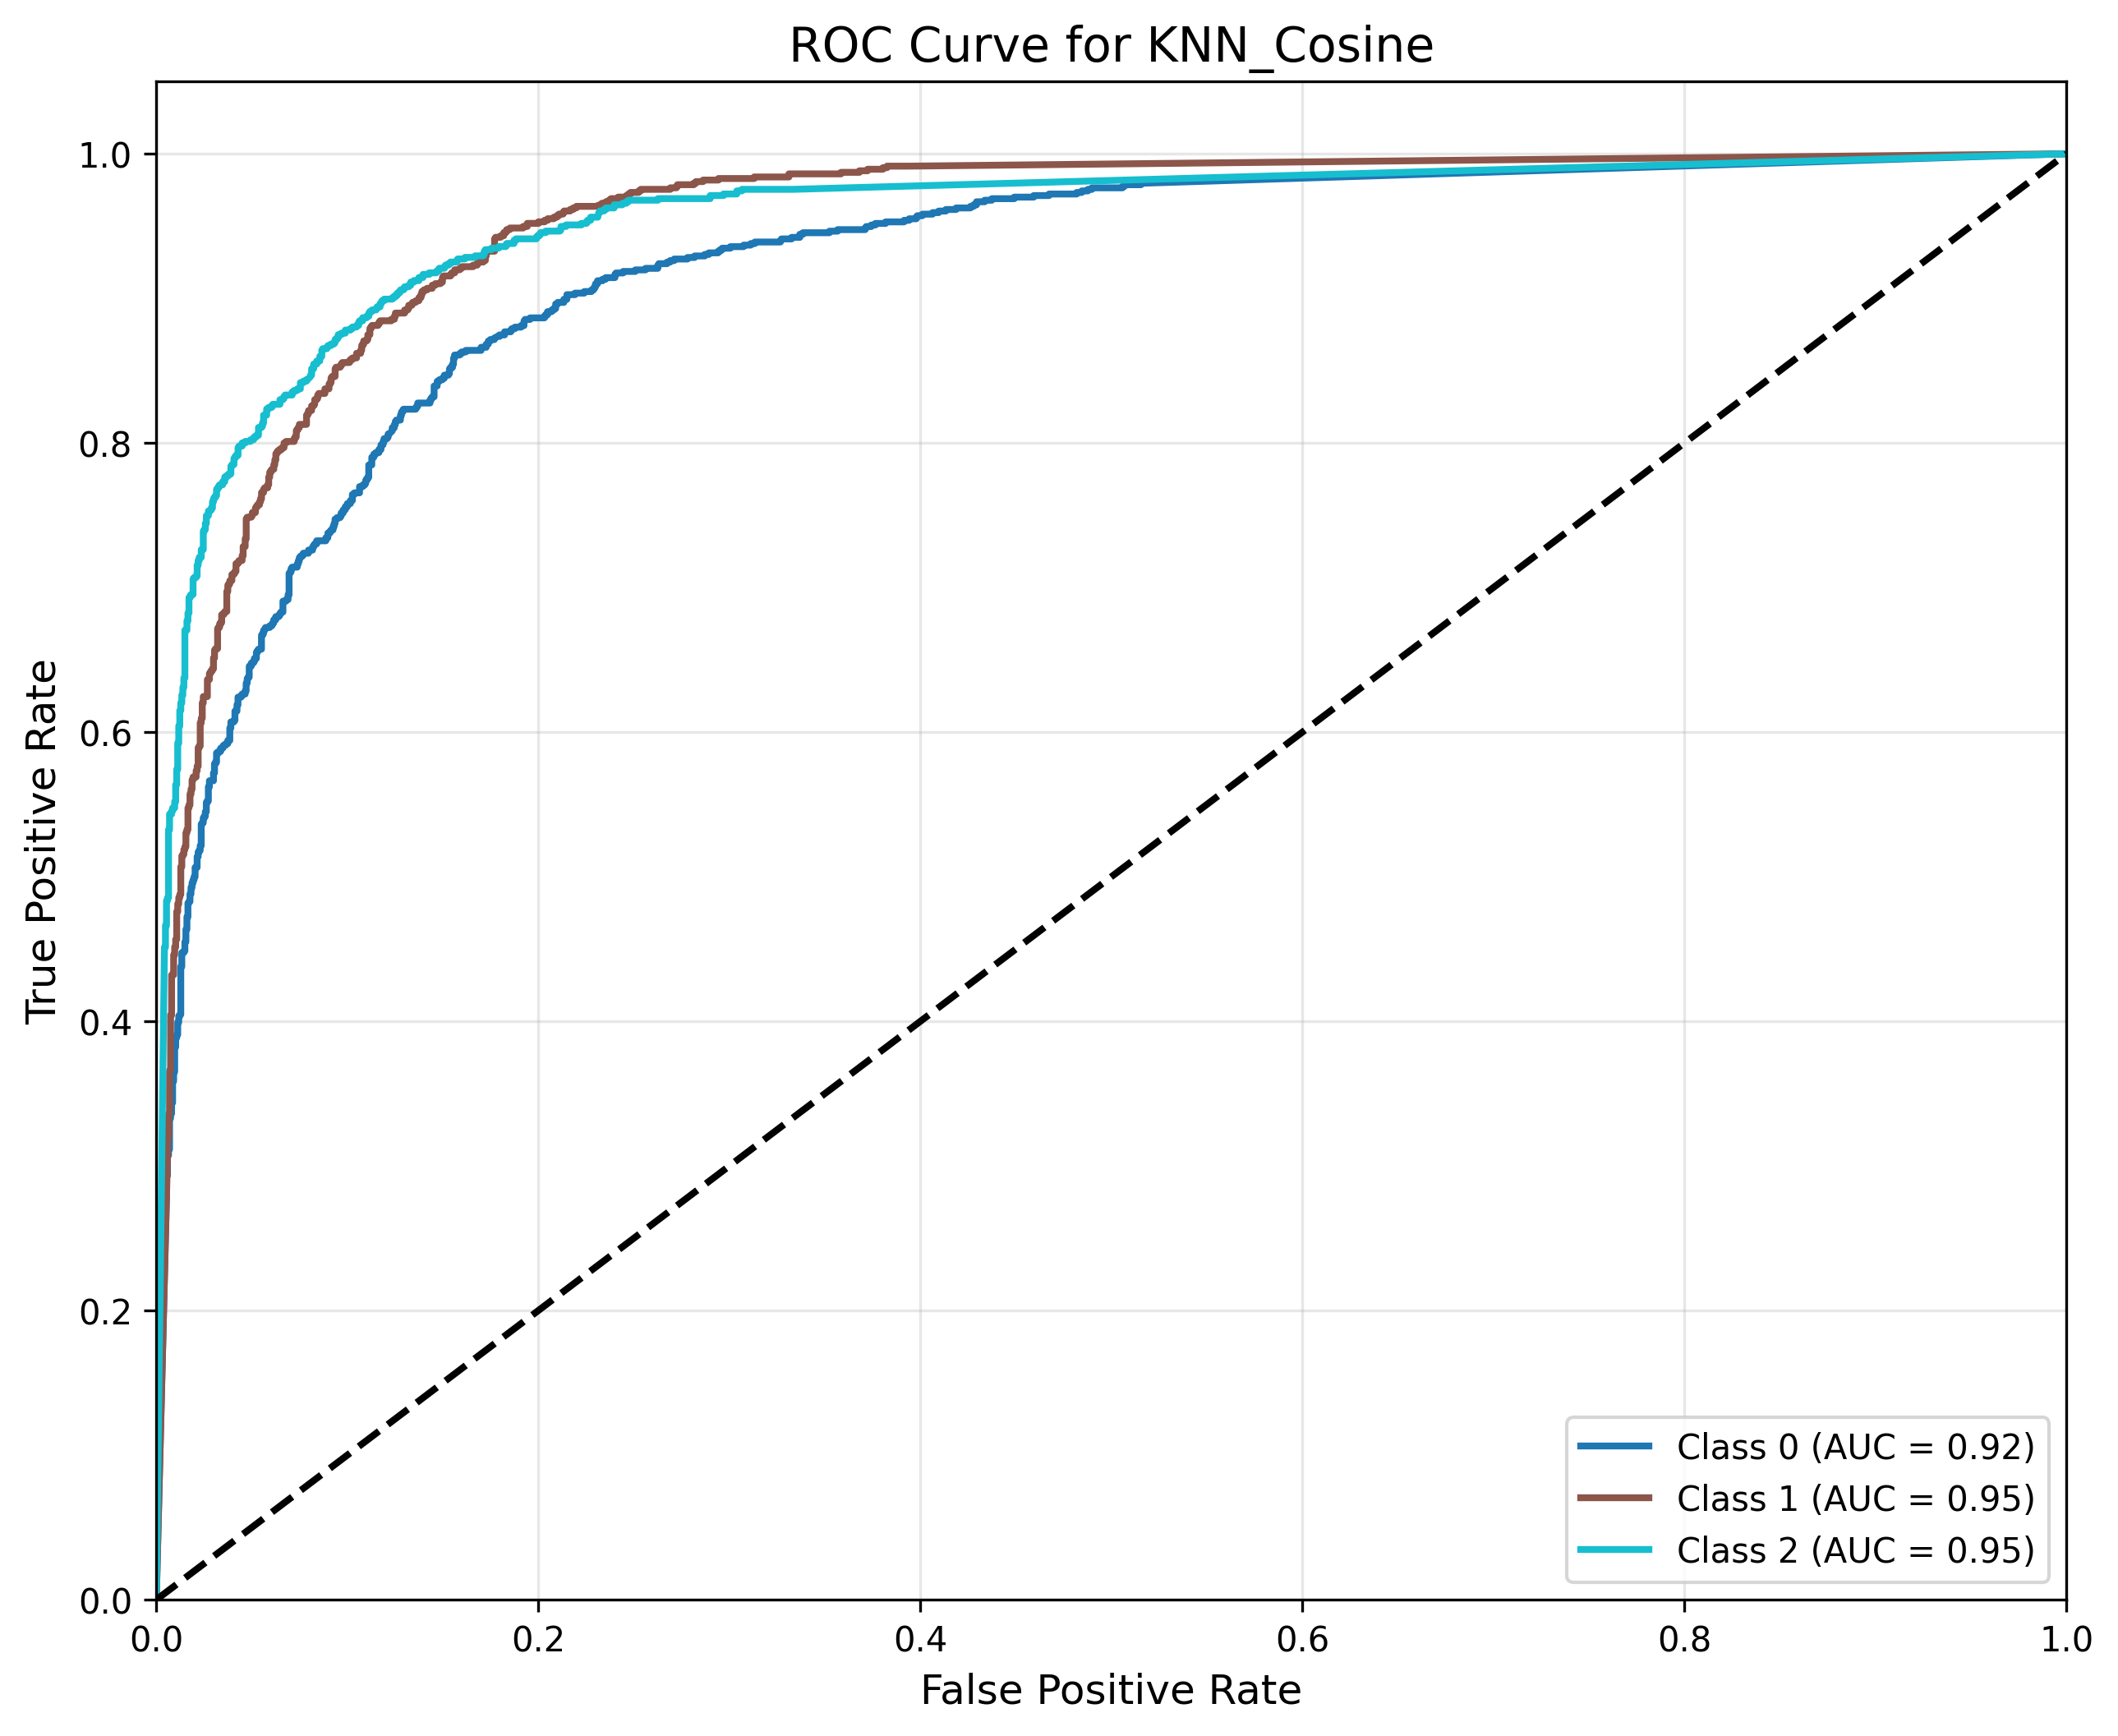
\includegraphics[width=\textwidth]{code/ResultsMainAugZip/plots/Block3_Probabilistic_Experiment_I/roc_curve_KNN_Cosine.png}
            \caption{ROC Curve}
        \end{subfigure}
    \end{figure}
    
    % Block 4: SVM Variants (Experiment I)
    \begin{figure}[!ht]
        \begin{subfigure}{0.5\textwidth}
            \centering
            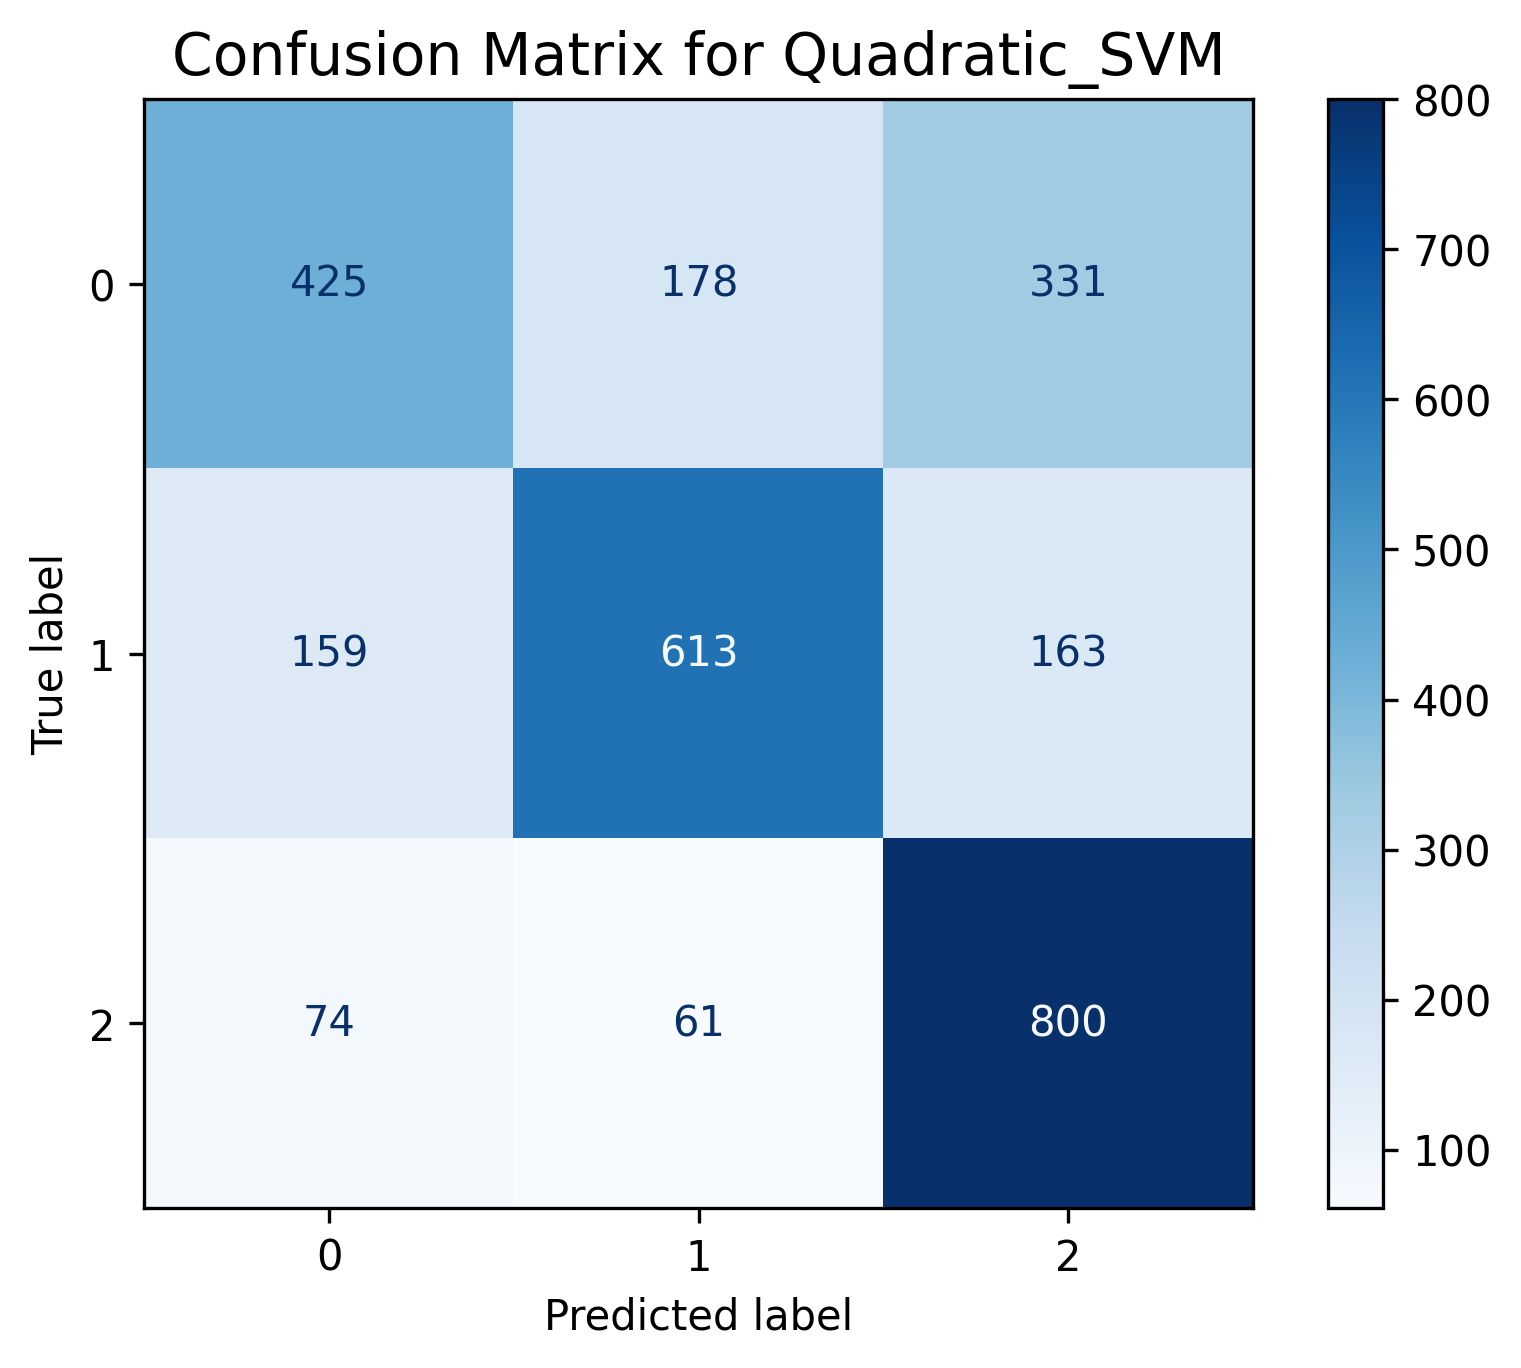
\includegraphics[width=0.9\textwidth]{code/ResultsMainAugZip/plots/Block4_SVM_Variants_Experiment_I/confusion_matrix_Quadratic_SVM.png}
            \caption{Confusion Matrix}
        \end{subfigure}
        \begin{subfigure}{0.5\textwidth}
            \centering
            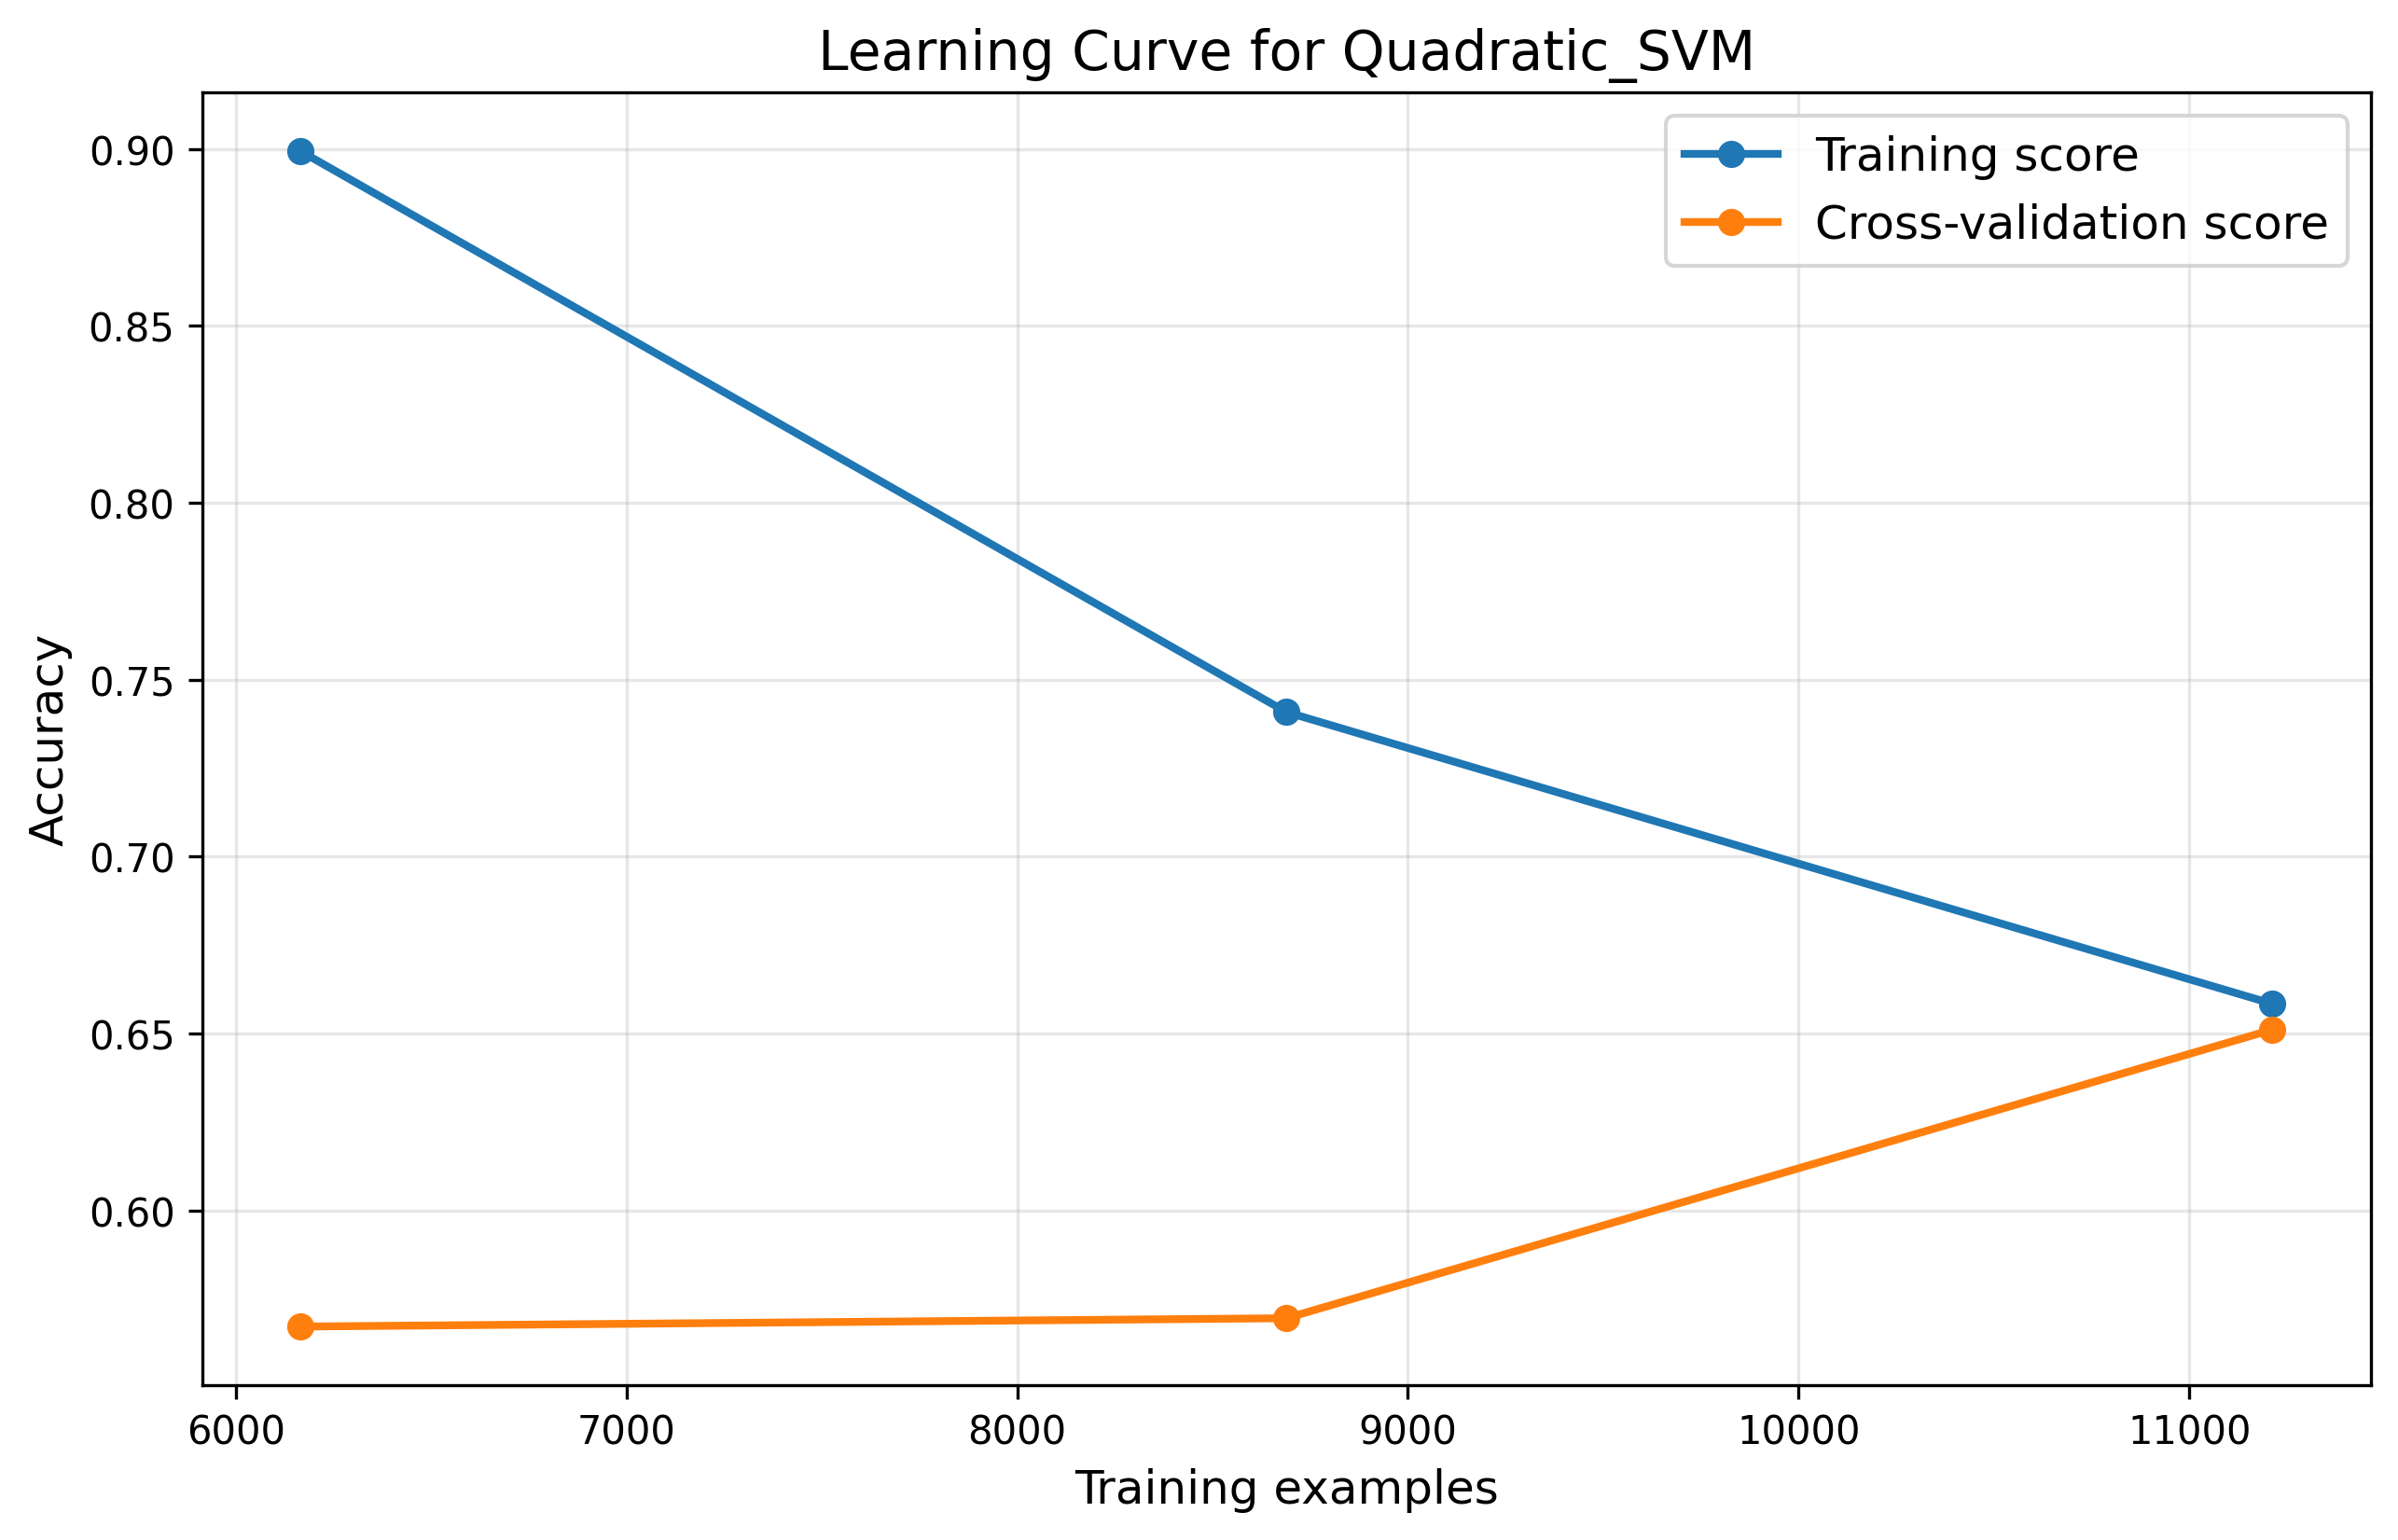
\includegraphics[width=0.9\textwidth]{code/ResultsMainAugZip/plots/Block4_SVM_Variants_Experiment_I/learning_curve_Quadratic_SVM.png}
            \caption{Learning Curve}
        \end{subfigure}
    \end{figure}
    
    % ==================== EXPERIMENT II PLOTS ====================
    % Block 1: Tree-Based (Experiment II)
    \begin{figure}[!ht]
        \begin{subfigure}{0.33\textwidth}
            \centering
            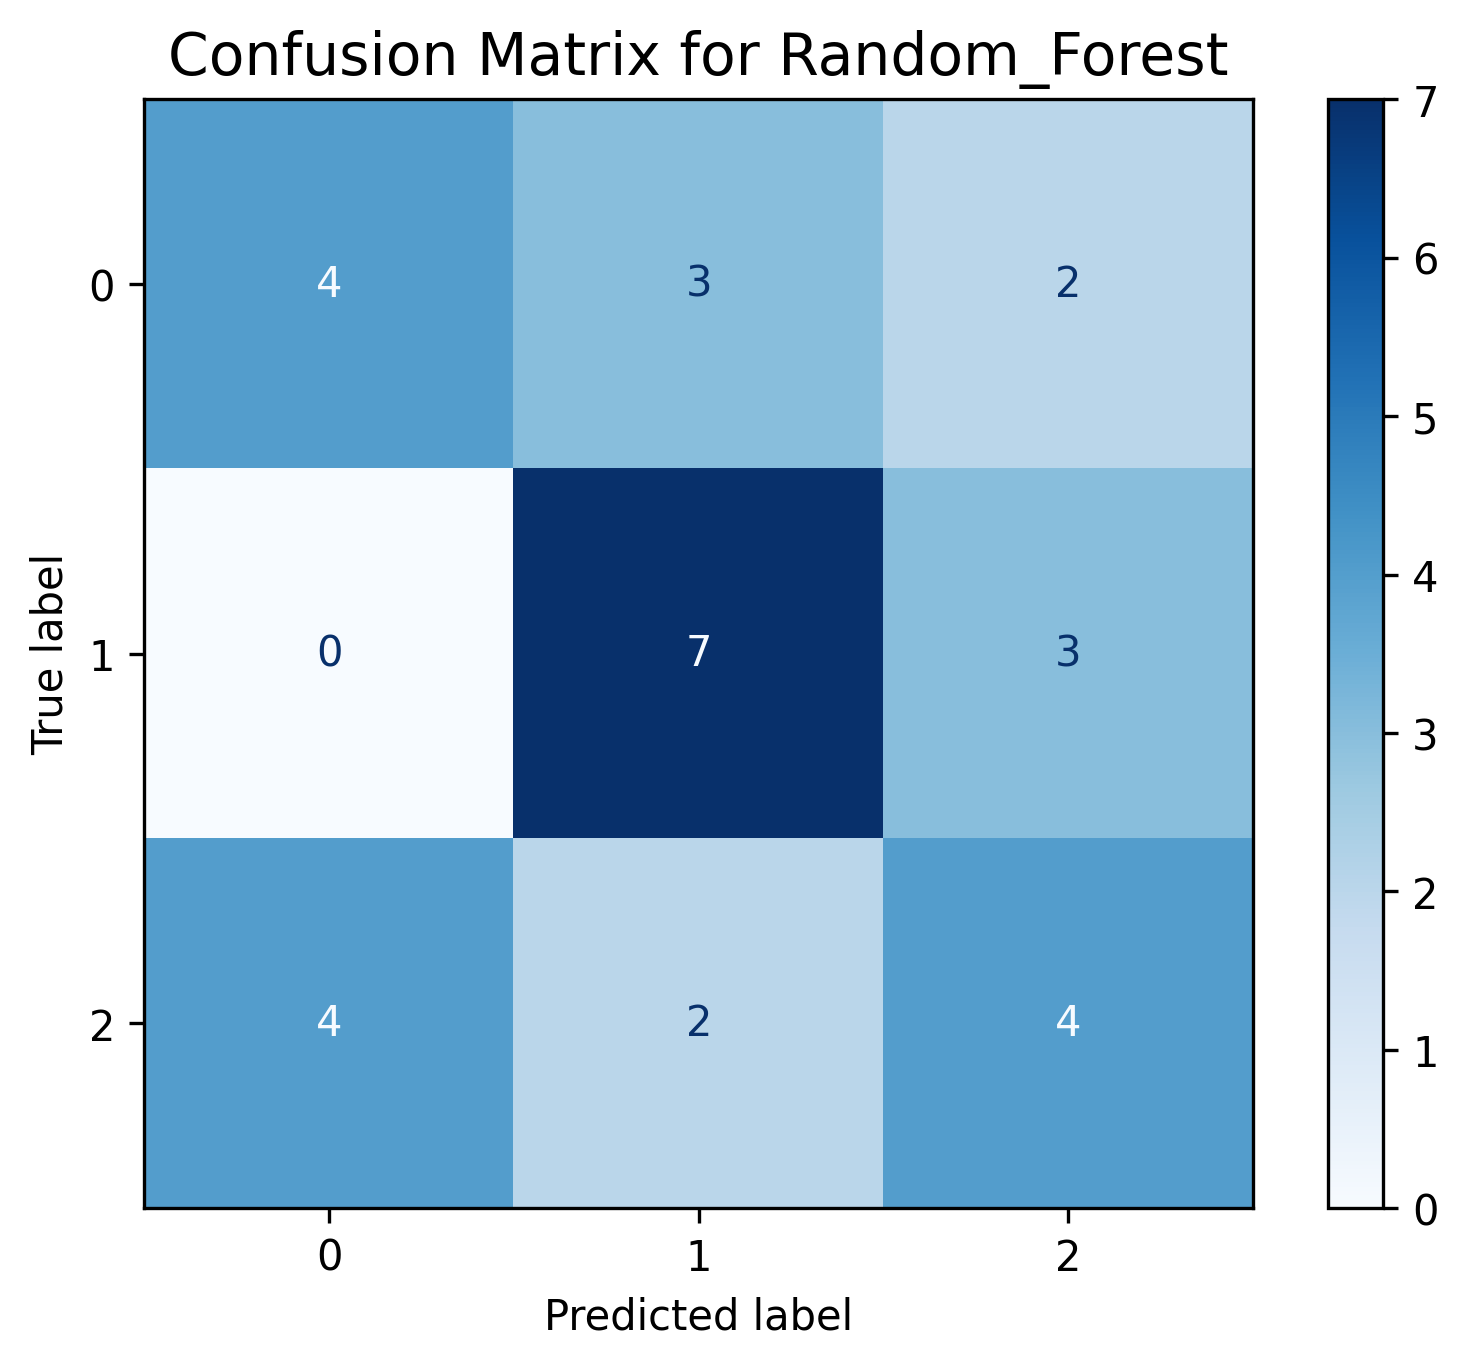
\includegraphics[width=\textwidth]{code/ResultsMainAugZip/plots/Block1_Tree_Based_Experiment_II/confusion_matrix_Random_Forest.png}
            \caption{Confusion Matrix}
        \end{subfigure}
        \begin{subfigure}{0.33\textwidth}
            \centering
            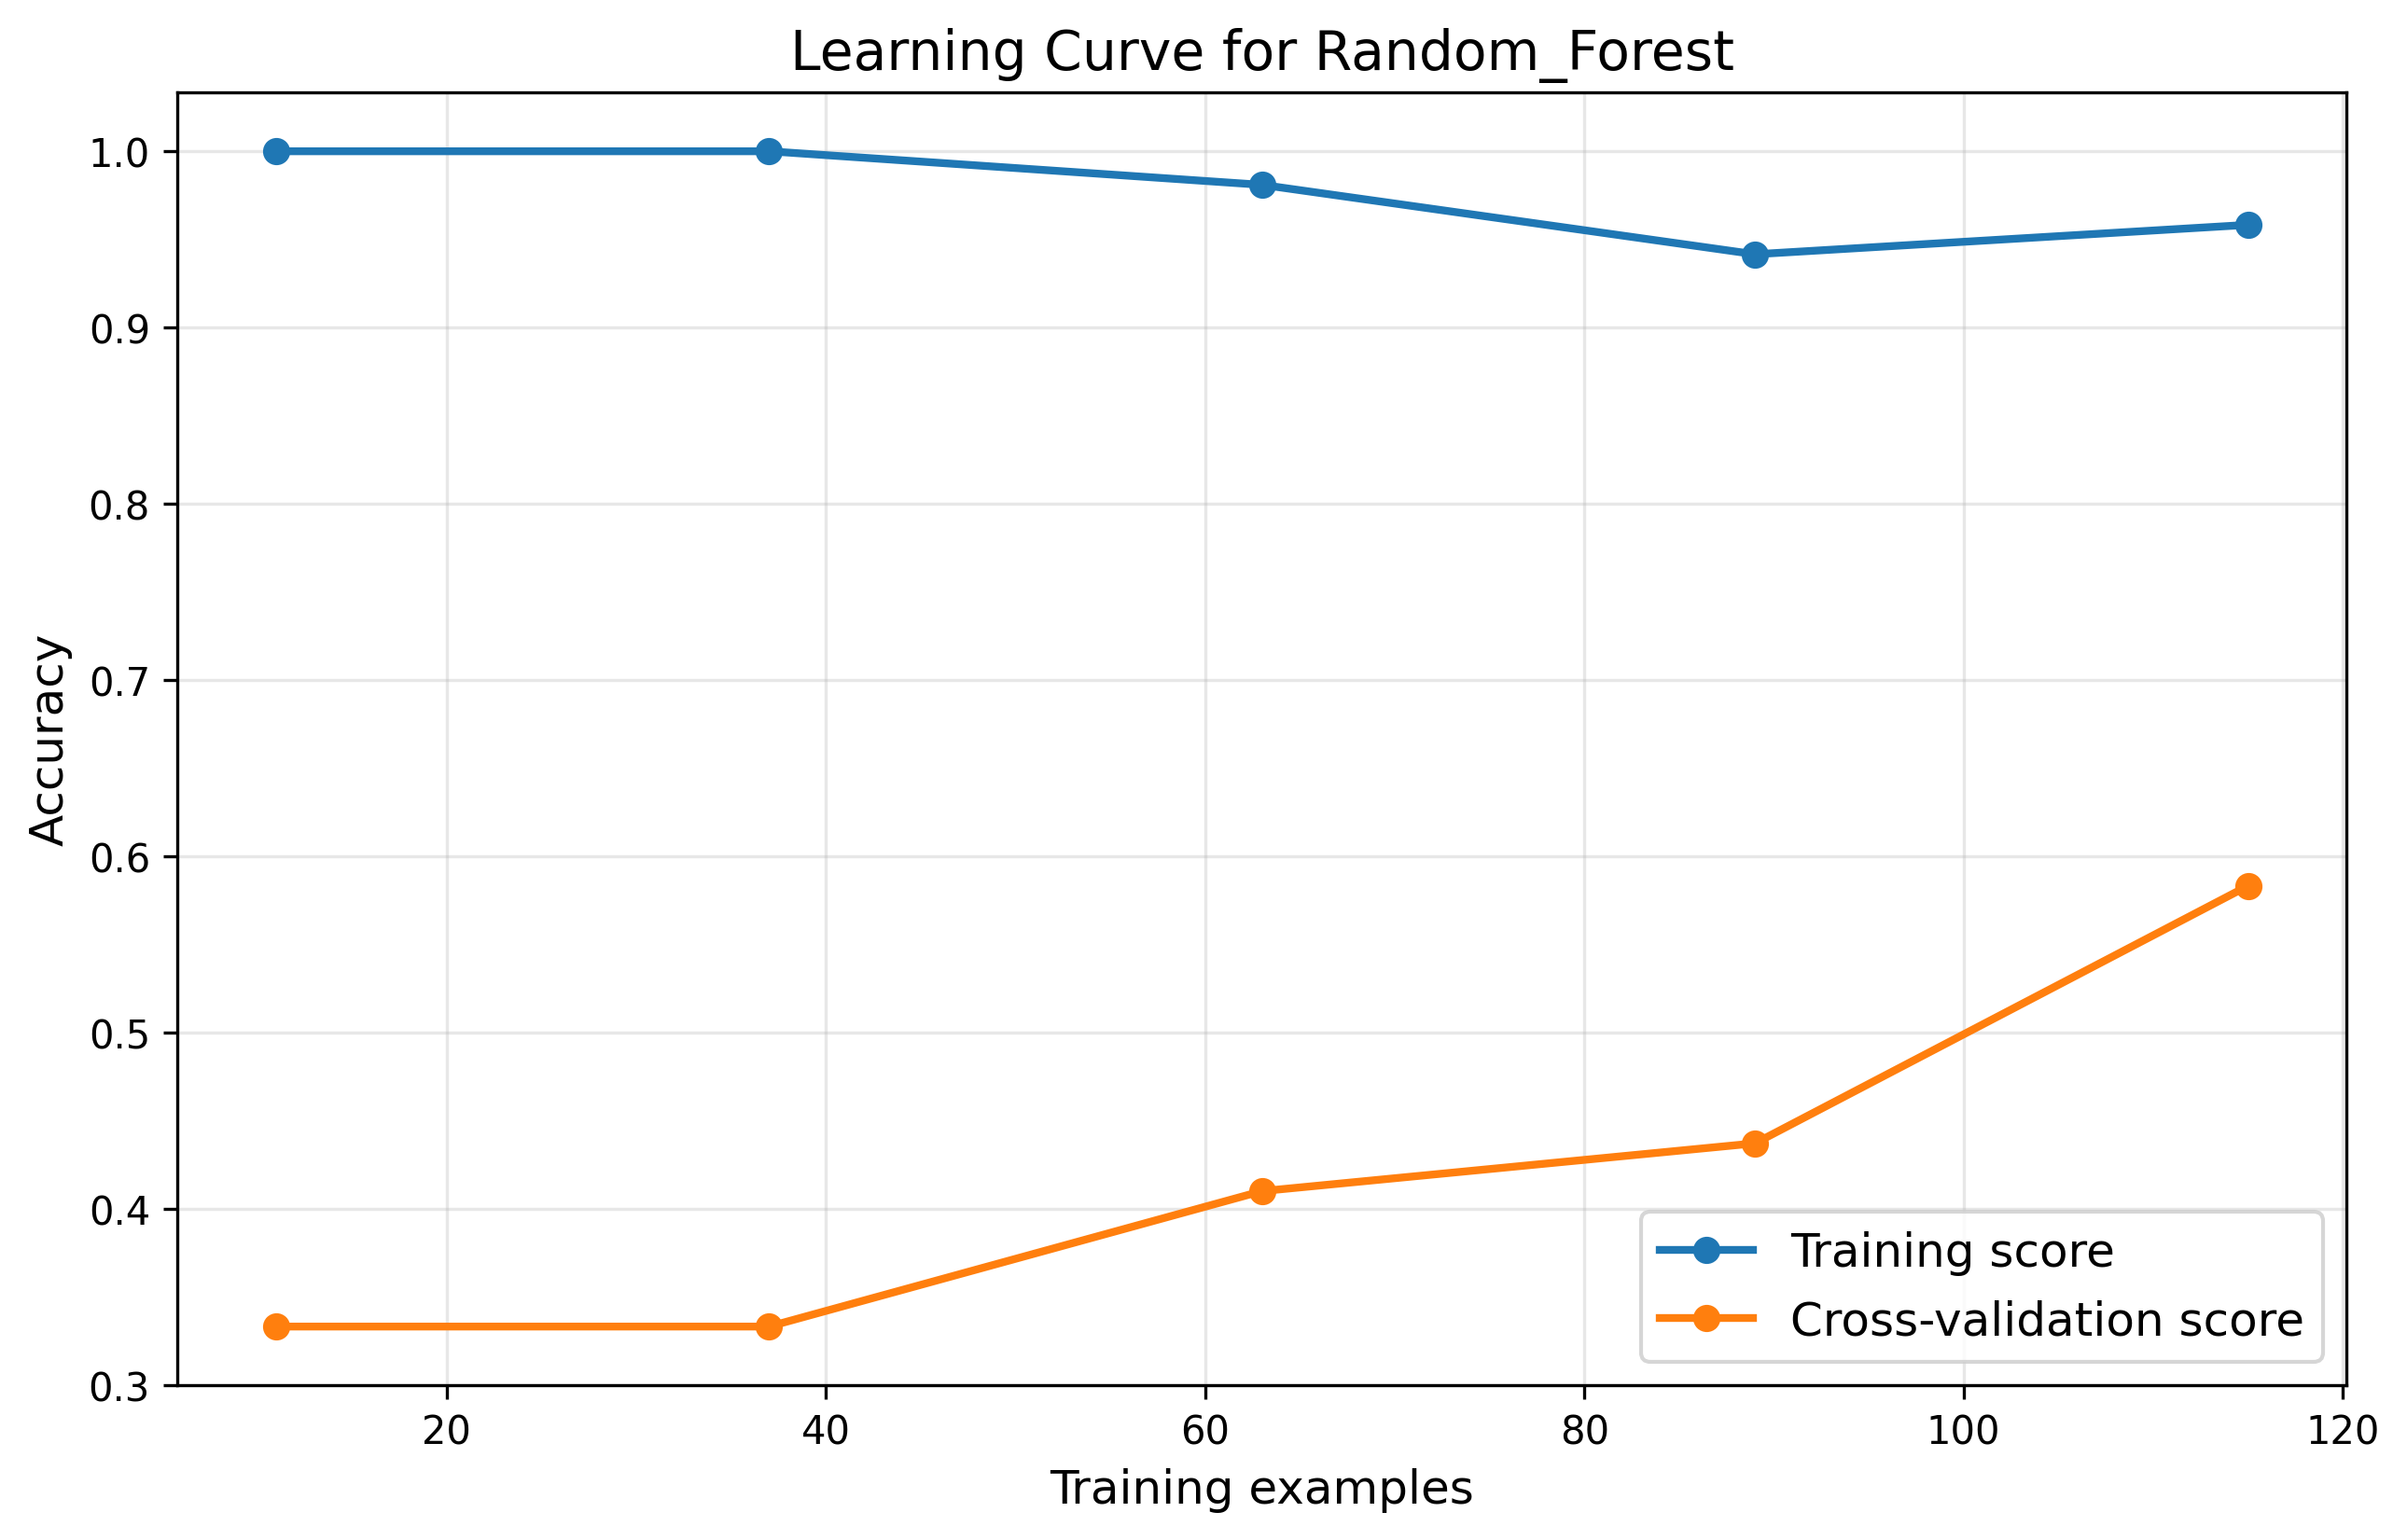
\includegraphics[width=\textwidth]{code/ResultsMainAugZip/plots/Block1_Tree_Based_Experiment_II/learning_curve_Random_Forest.png}
            \caption{Learning Curve}
        \end{subfigure}
        \begin{subfigure}{0.33\textwidth}
            \centering
            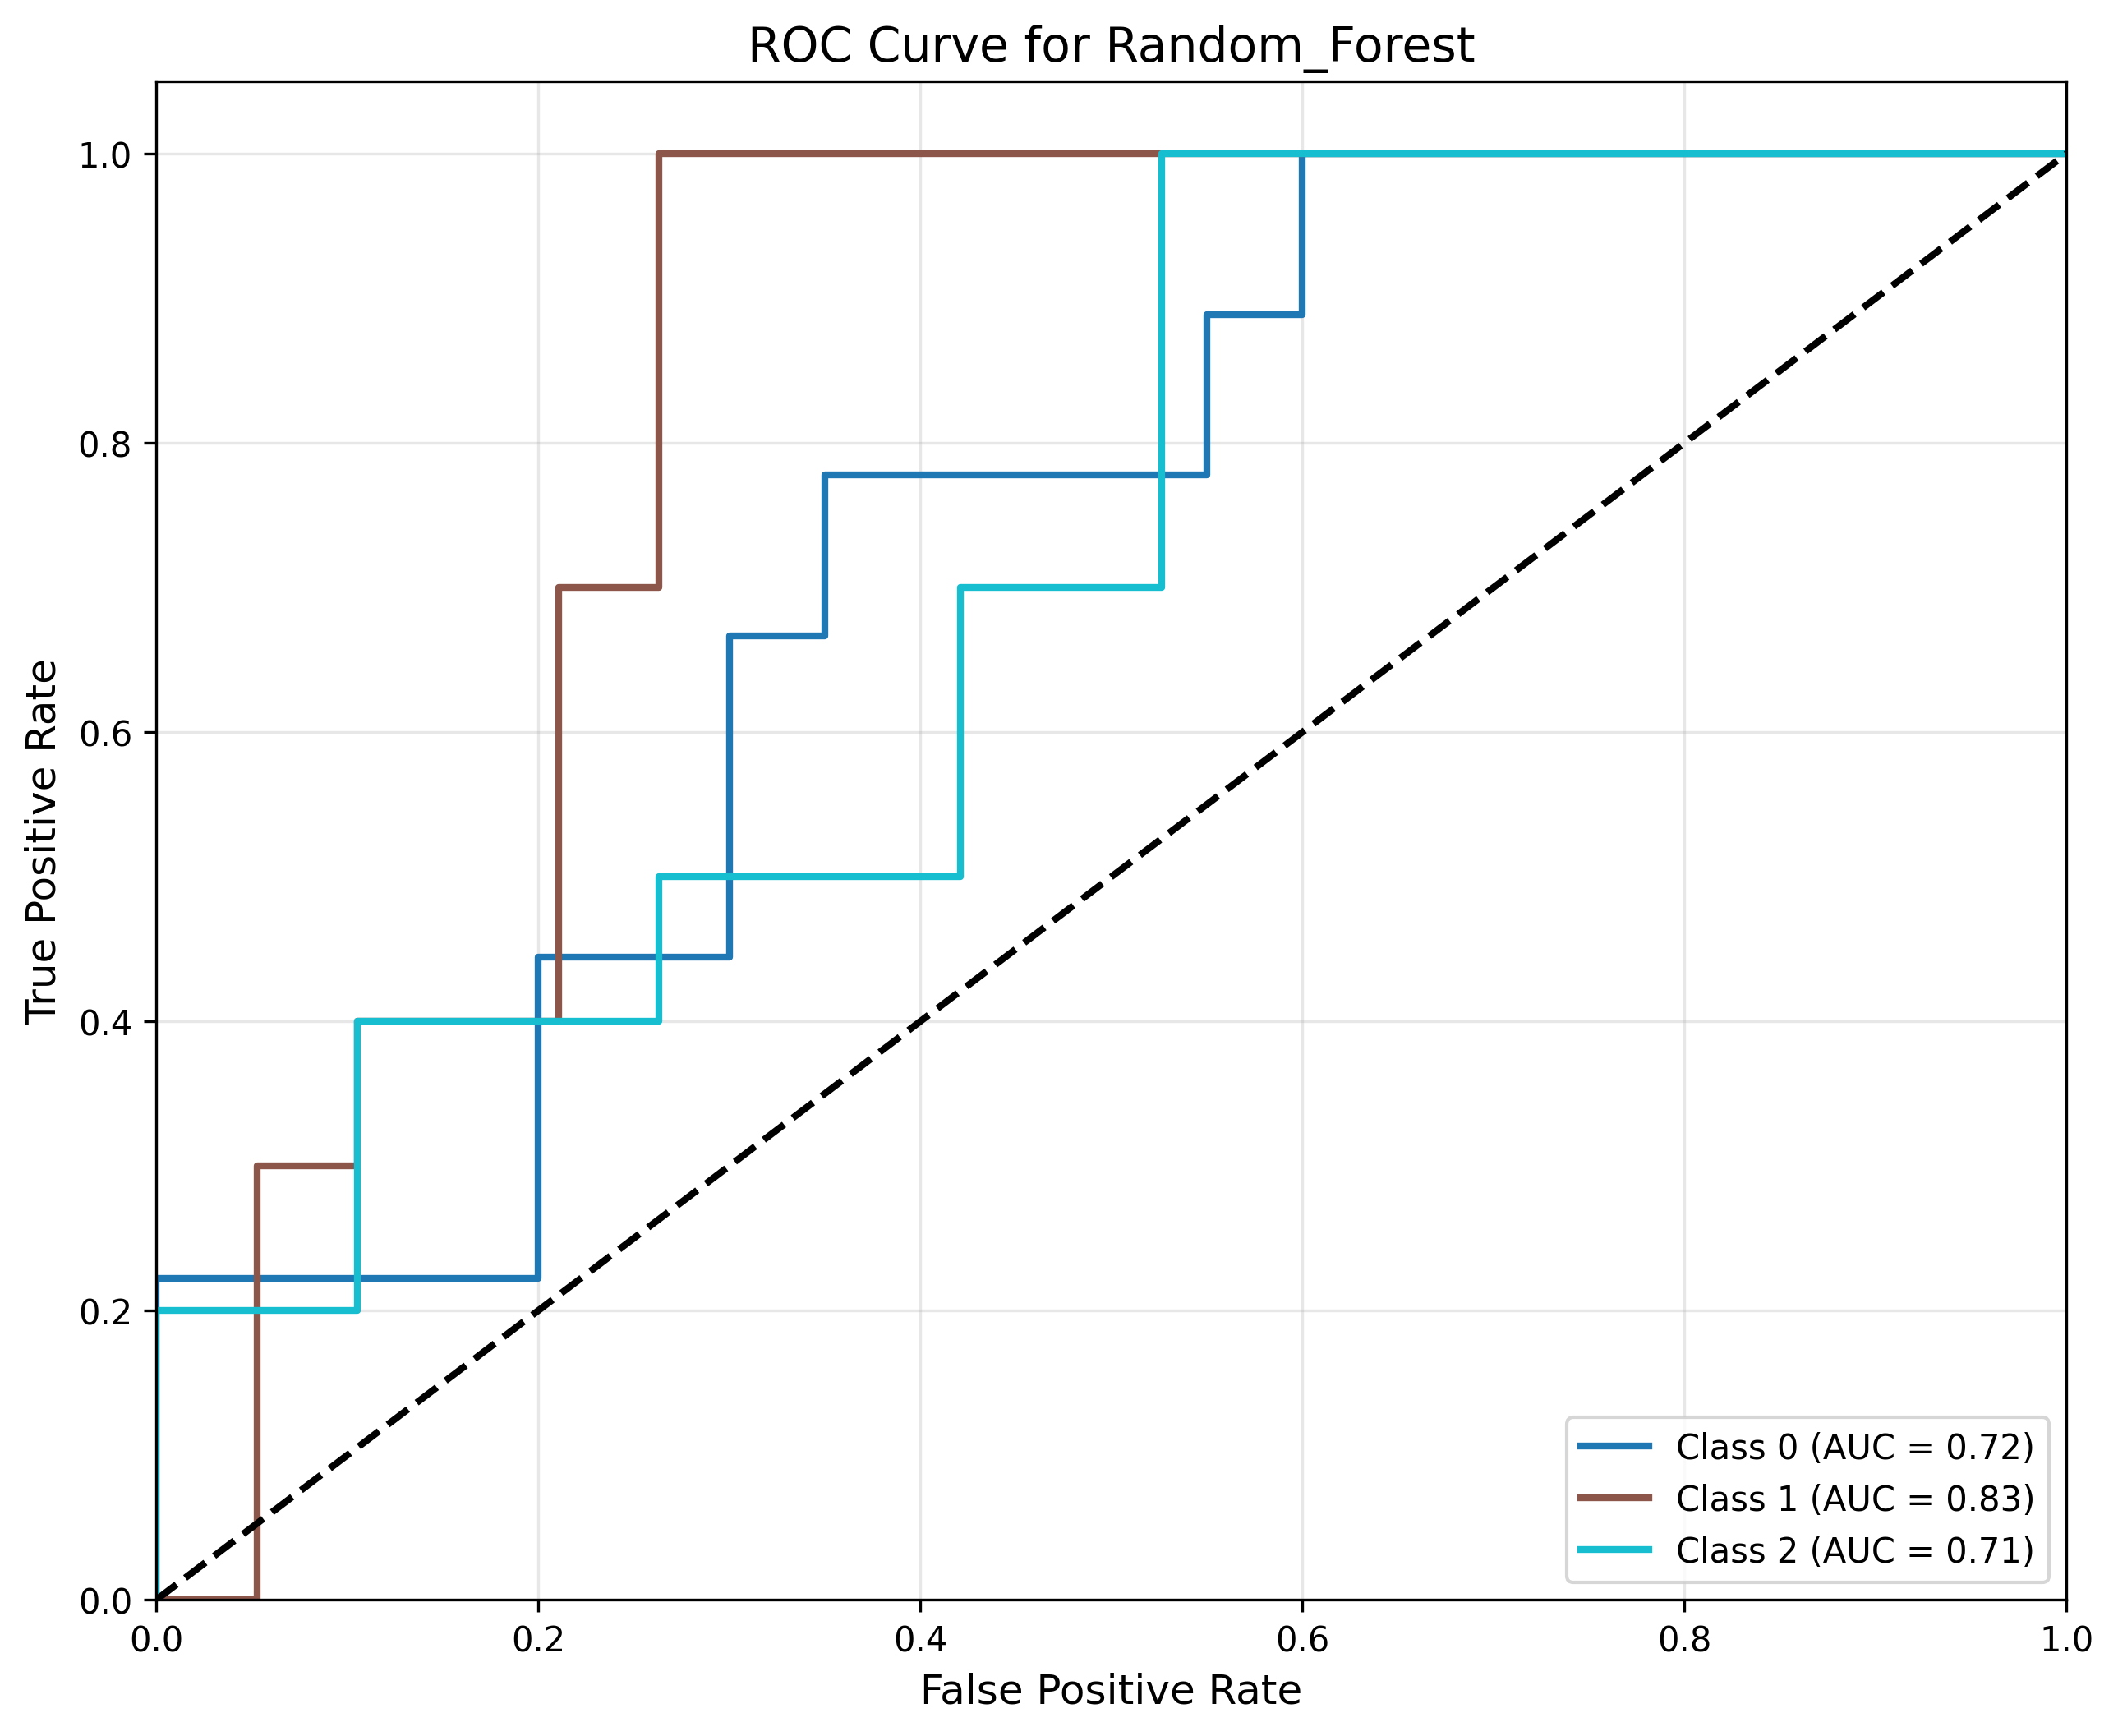
\includegraphics[width=\textwidth]{code/ResultsMainAugZip/plots/Block1_Tree_Based_Experiment_II/roc_curve_Random_Forest.png}
            \caption{ROC Curve}
        \end{subfigure}
    \end{figure}
    
    % Block 2: KNN Variants (Experiment II)
    \begin{figure}[!ht]
        \begin{subfigure}{0.33\textwidth}
            \centering
            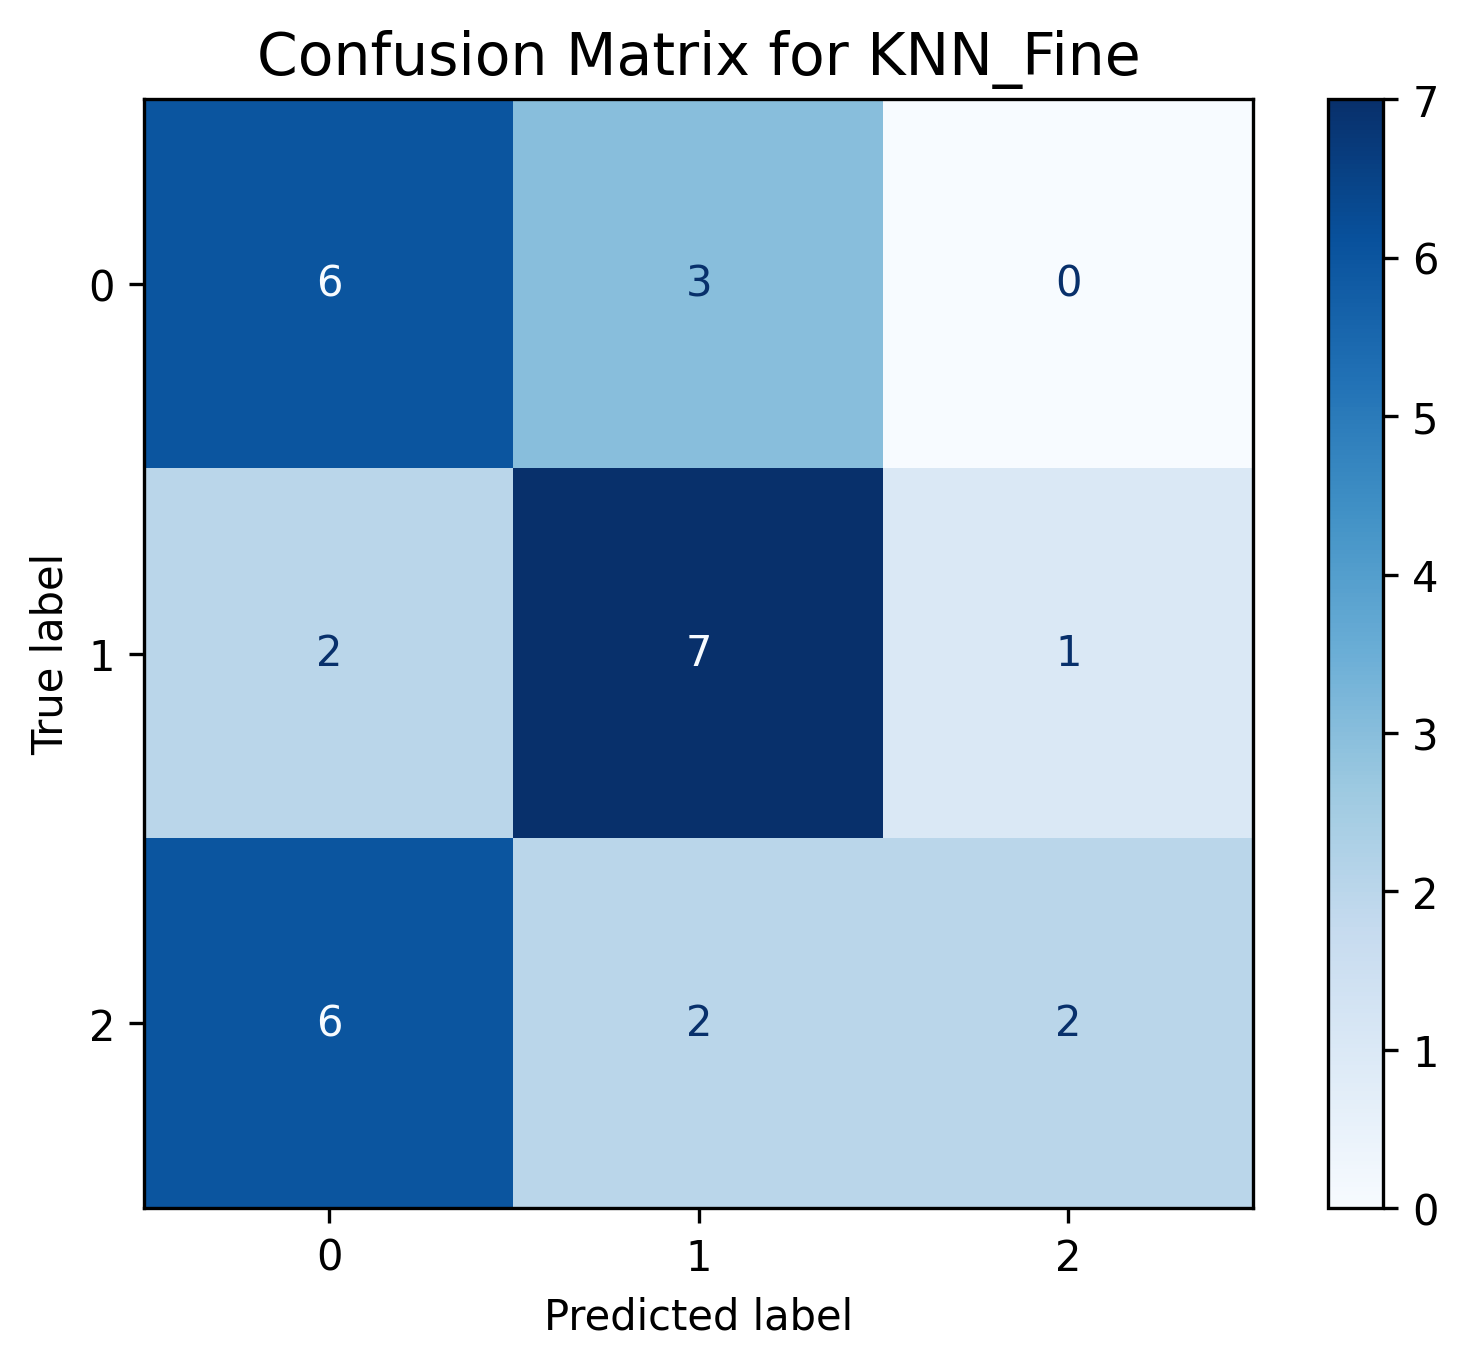
\includegraphics[width=\textwidth]{code/ResultsMainAugZip/plots/Block2_KNN_Variants_Experiment_II/confusion_matrix_KNN_Fine.png}
            \caption{Confusion Matrix}
        \end{subfigure}
        \begin{subfigure}{0.33\textwidth}
            \centering
            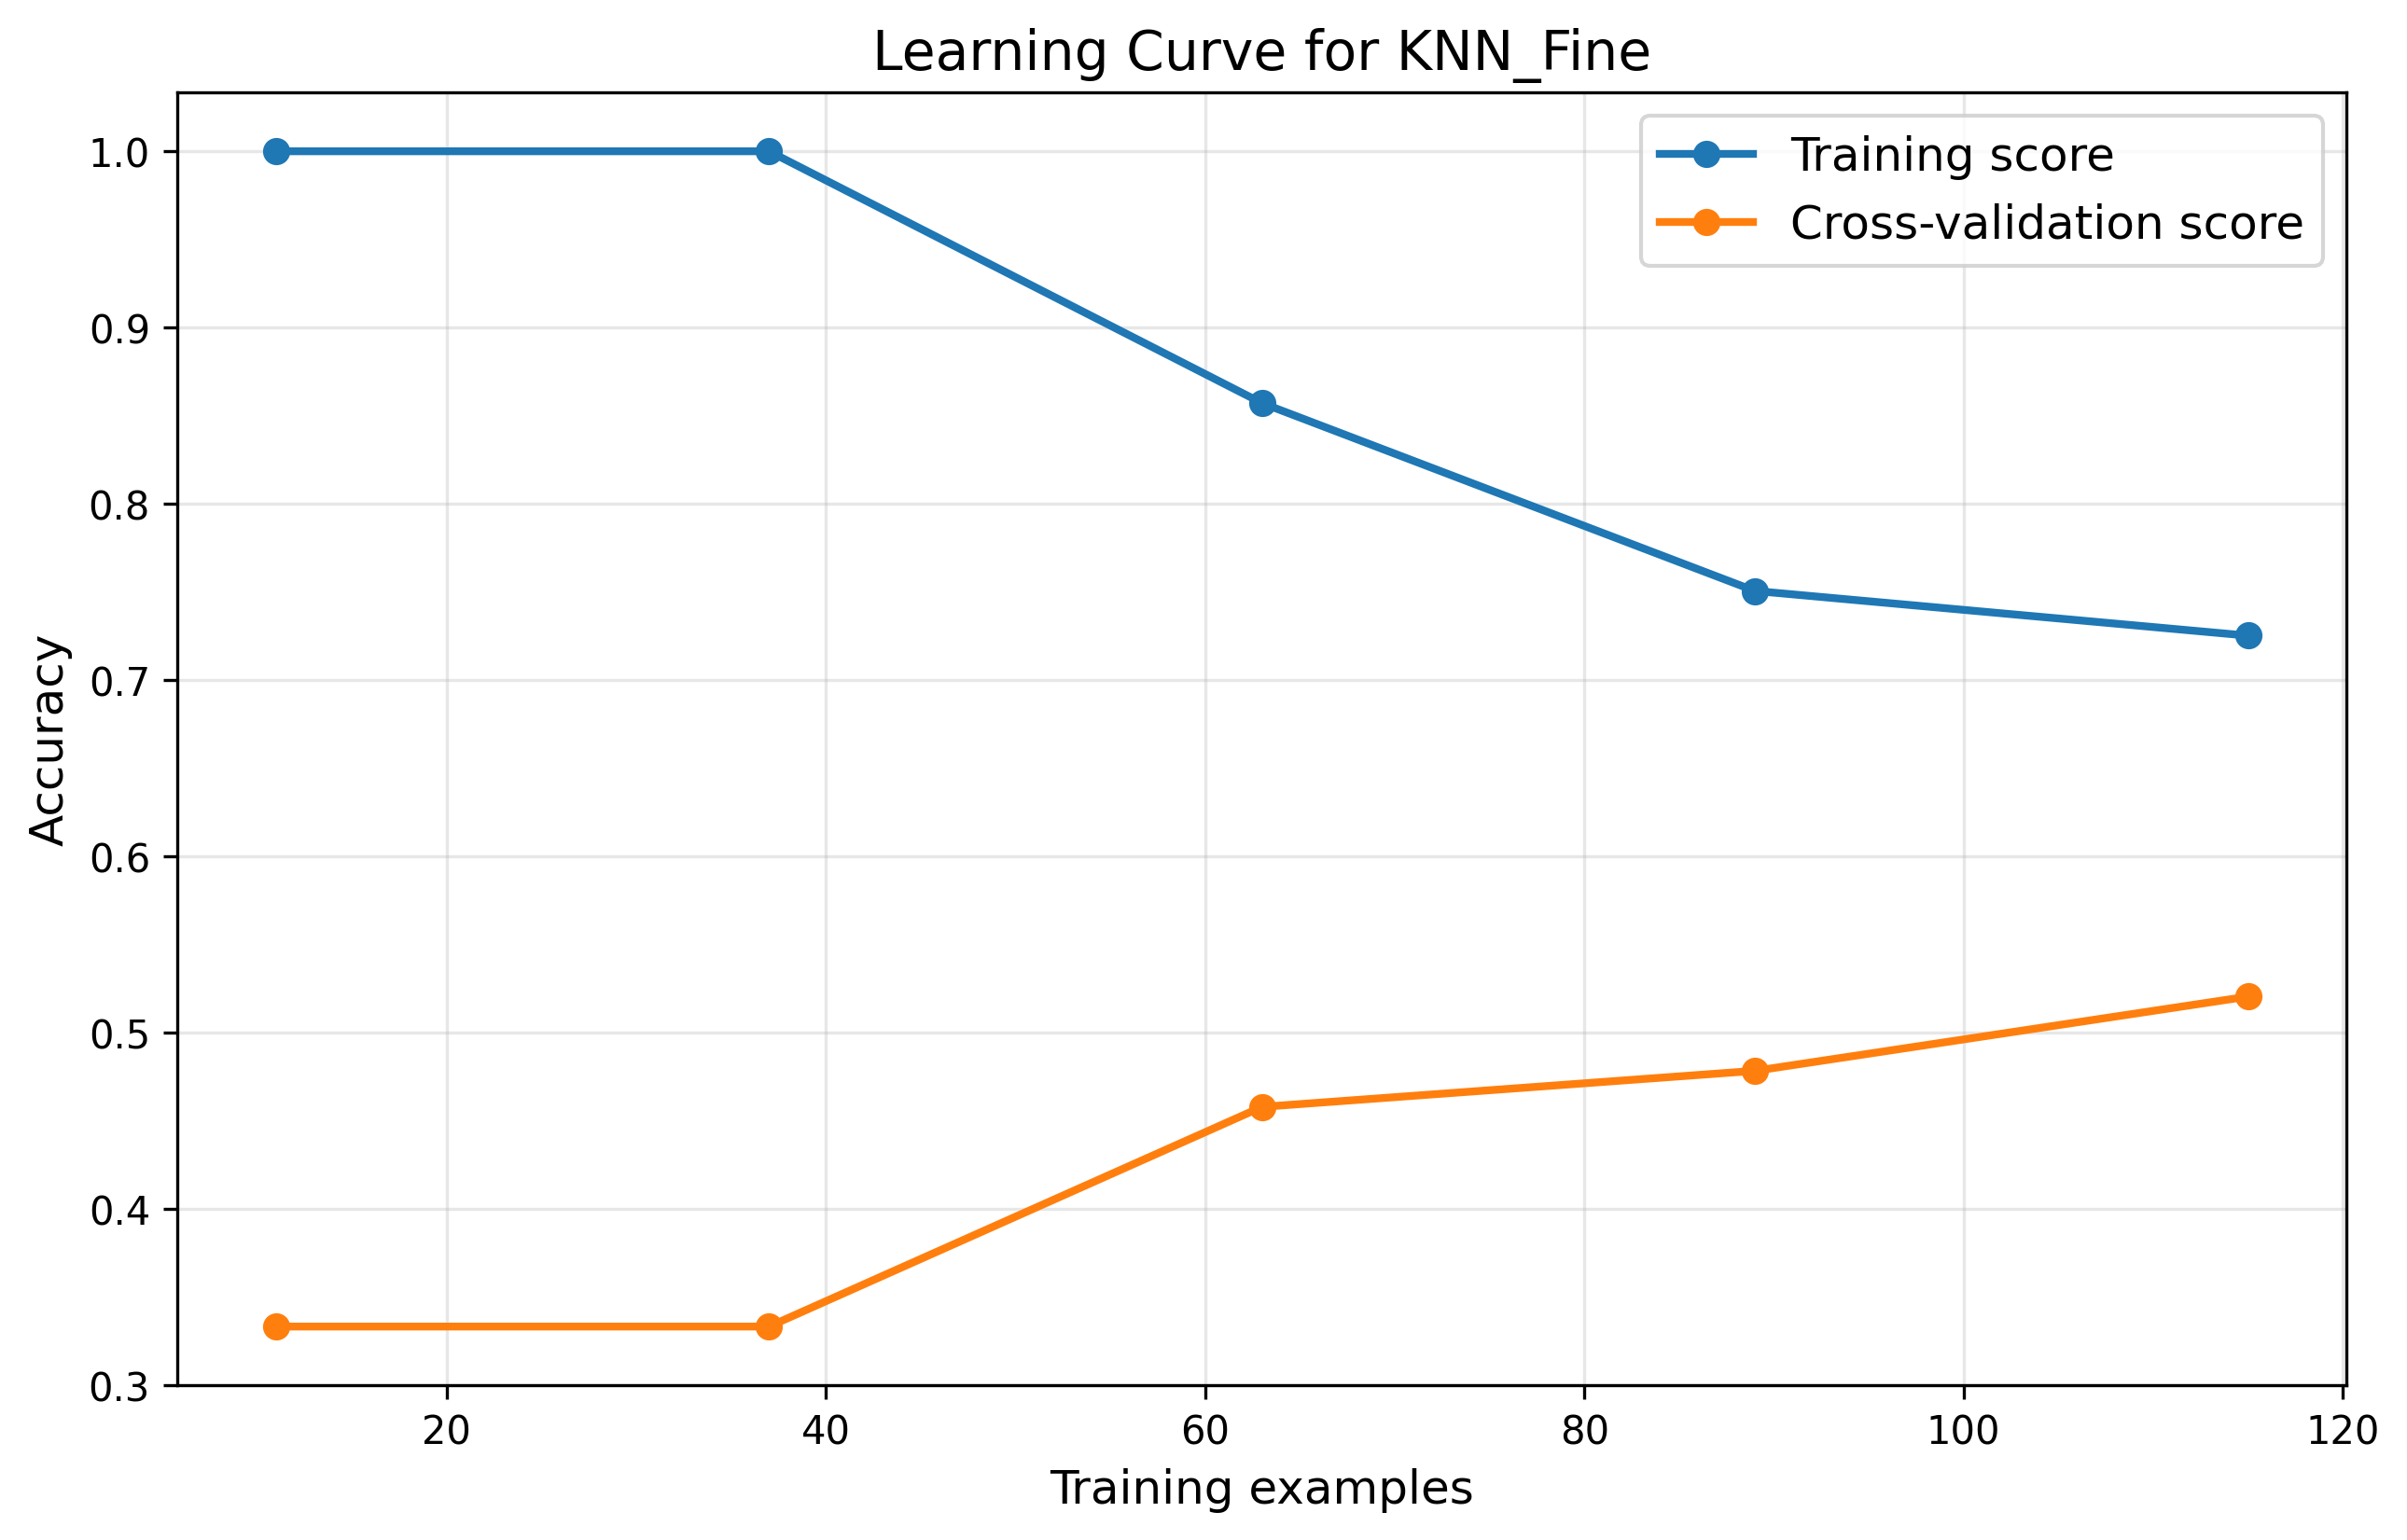
\includegraphics[width=\textwidth]{code/ResultsMainAugZip/plots/Block2_KNN_Variants_Experiment_II/learning_curve_KNN_Fine.png}
            \caption{Learning Curve}
        \end{subfigure}
        \begin{subfigure}{0.33\textwidth}
            \centering
            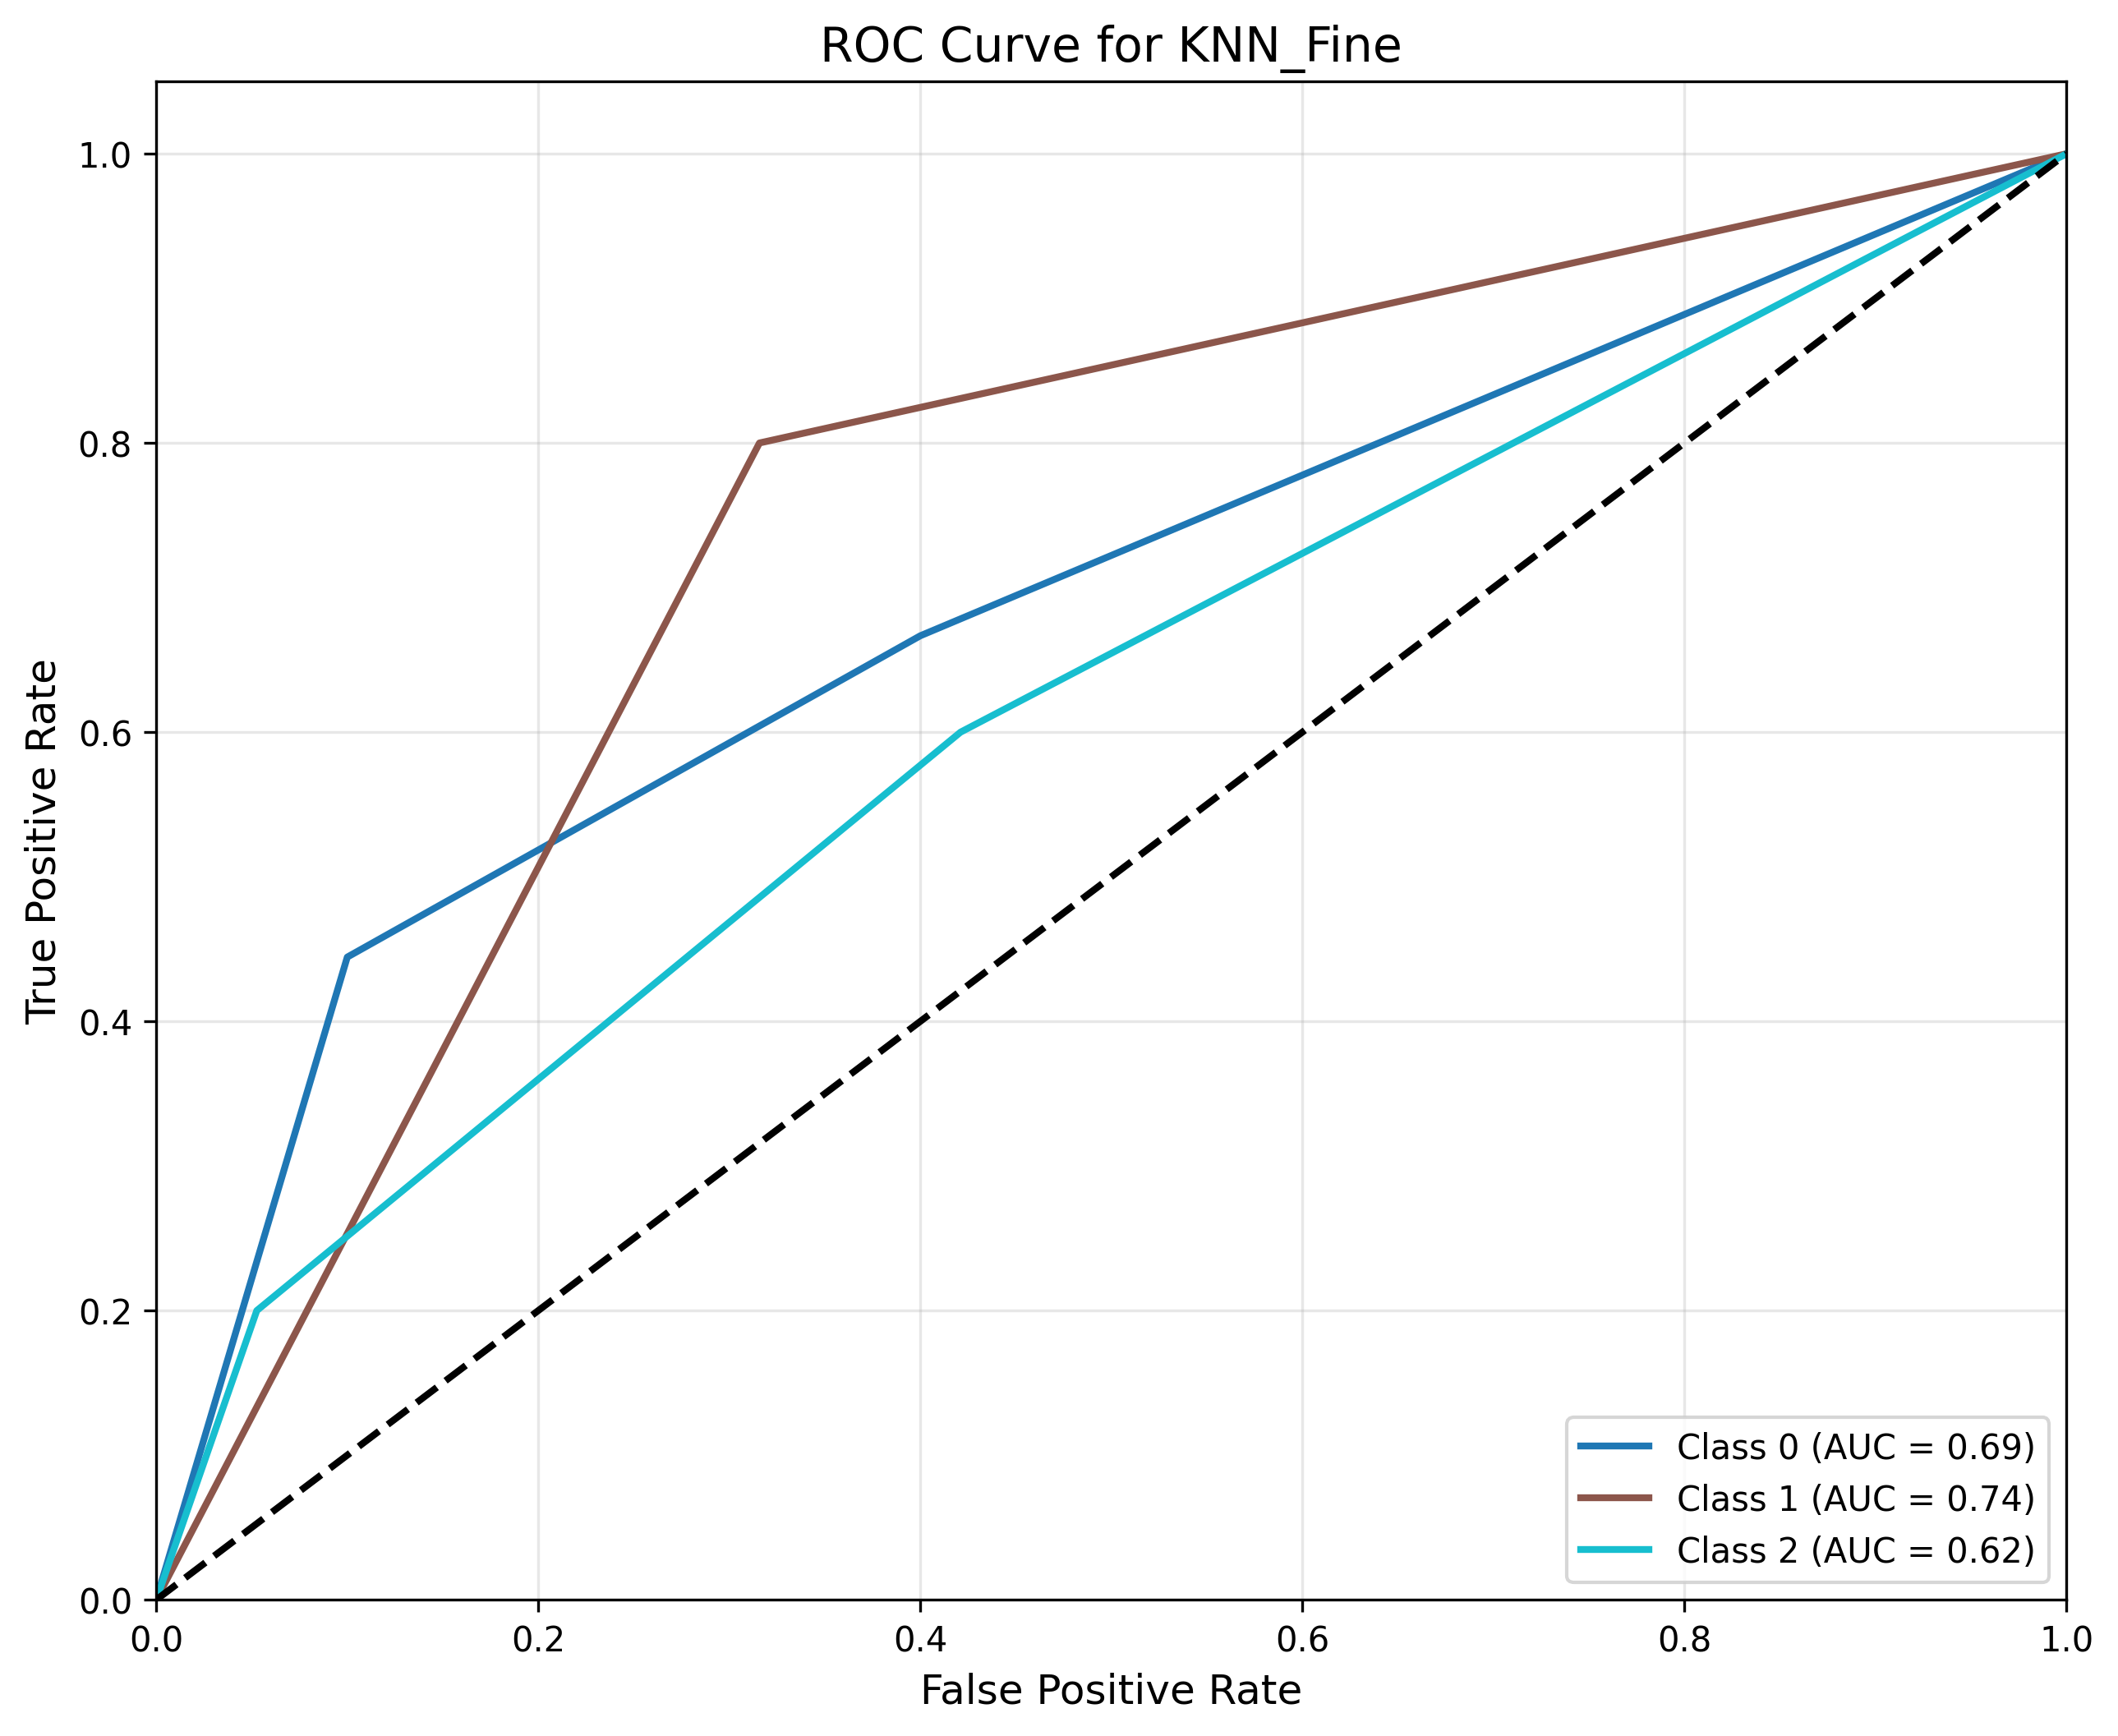
\includegraphics[width=\textwidth]{code/ResultsMainAugZip/plots/Block2_KNN_Variants_Experiment_II/roc_curve_KNN_Fine.png}
            \caption{ROC Curve}
        \end{subfigure}
    \end{figure}
    
    % Block 3: Probabilistic (Experiment II)
    \begin{figure}[!ht]
        \begin{subfigure}{0.33\textwidth}
            \centering
            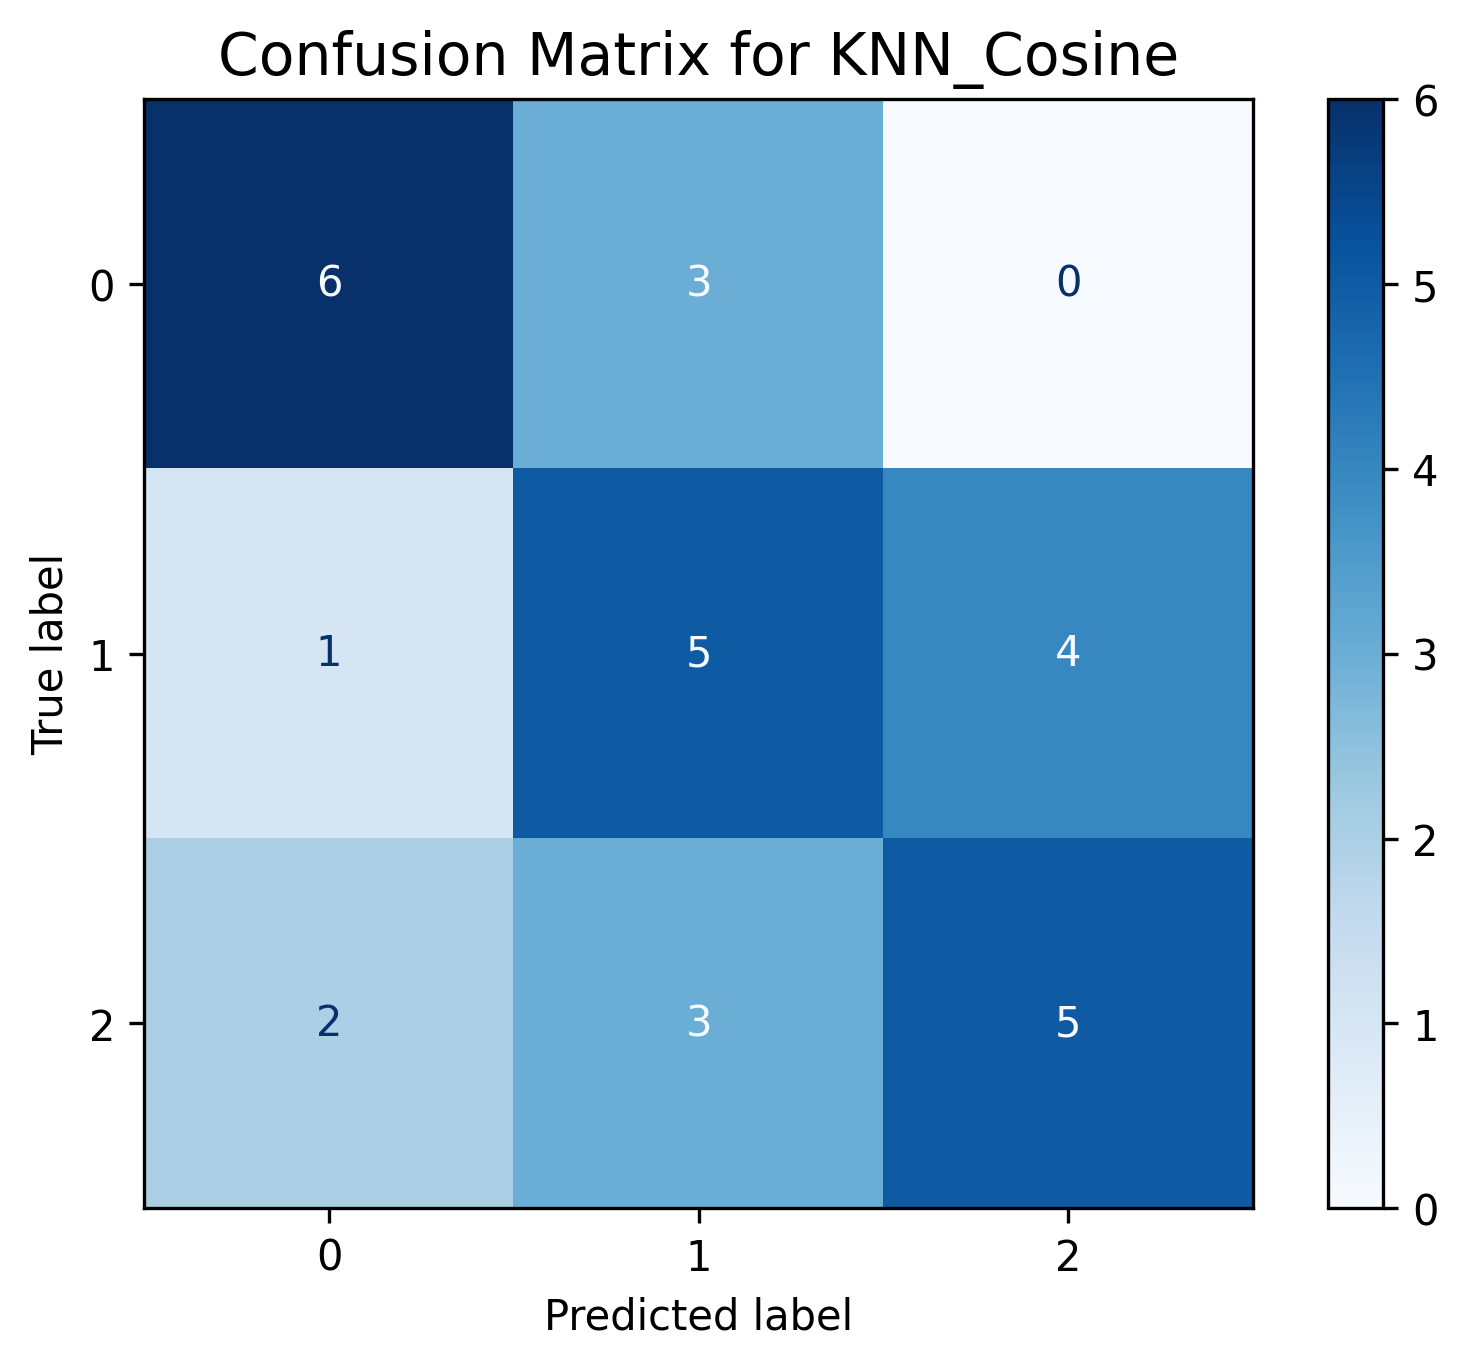
\includegraphics[width=\textwidth]{code/ResultsMainAugZip/plots/Block3_Probabilistic_Experiment_II/confusion_matrix_KNN_Cosine.png}
            \caption{Confusion Matrix}
        \end{subfigure}
        \begin{subfigure}{0.33\textwidth}
            \centering
            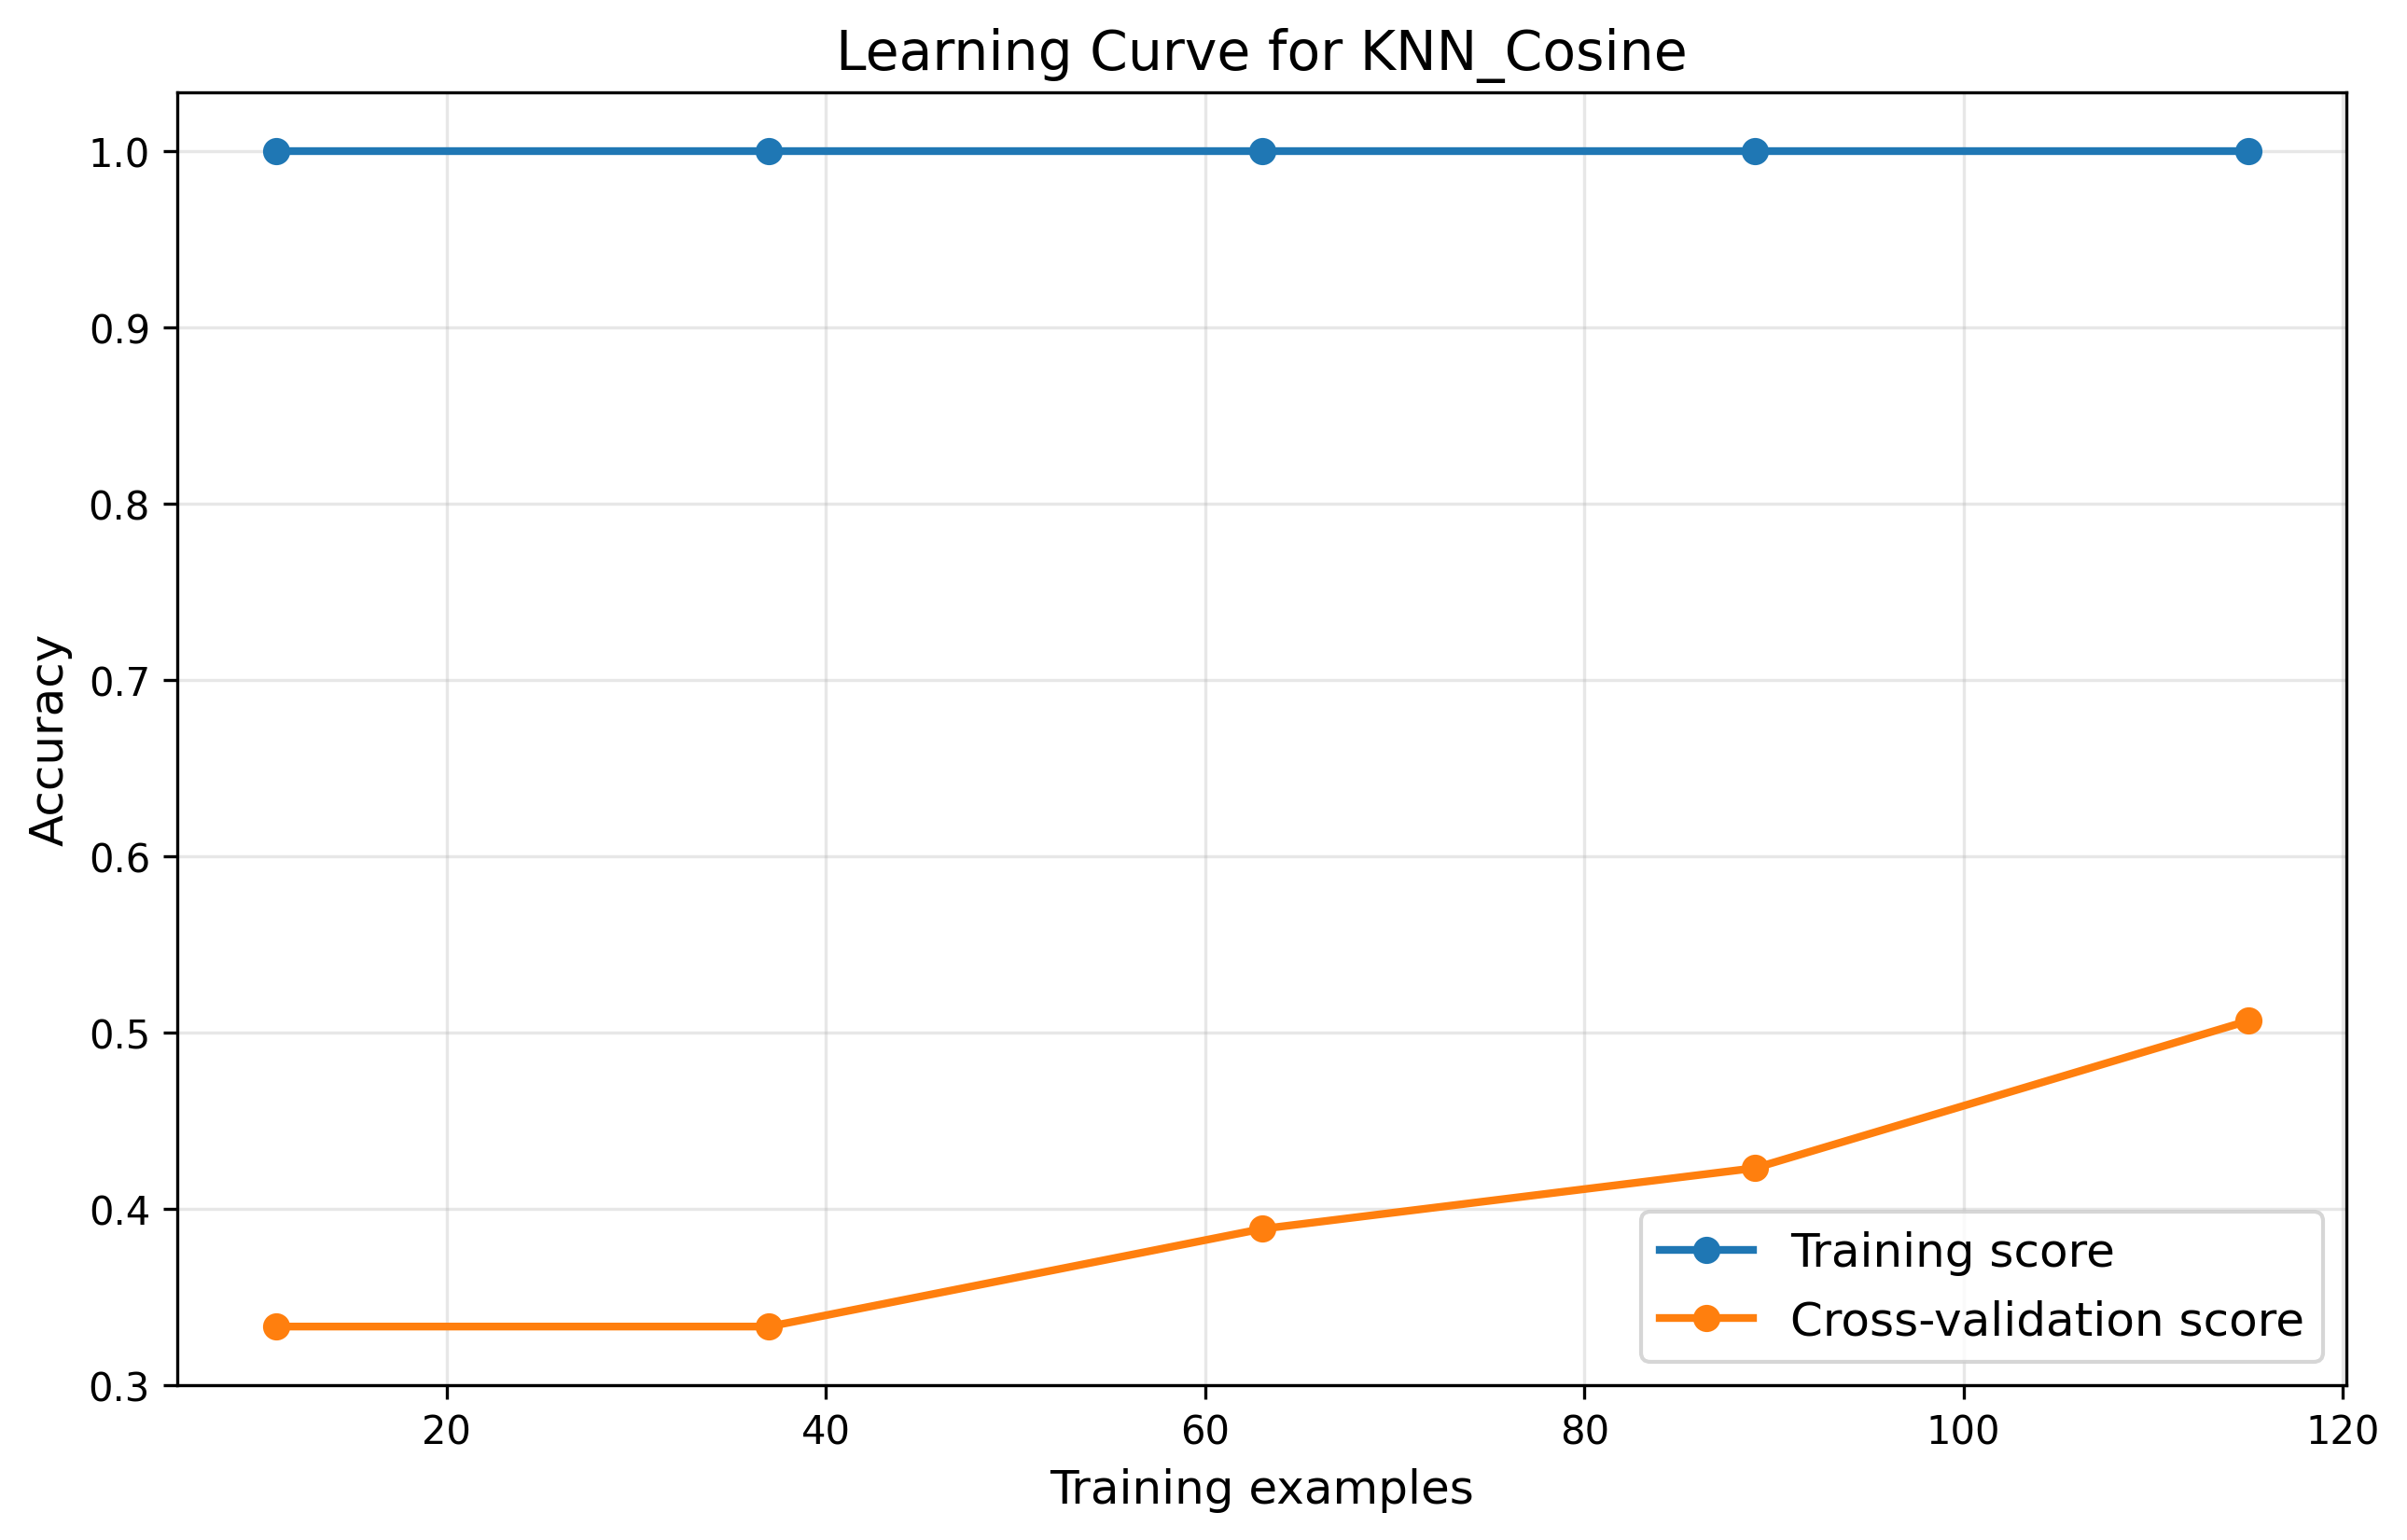
\includegraphics[width=\textwidth]{code/ResultsMainAugZip/plots/Block3_Probabilistic_Experiment_II/learning_curve_KNN_Cosine.png}
            \caption{Learning Curve}
        \end{subfigure}
        \begin{subfigure}{0.33\textwidth}
            \centering
            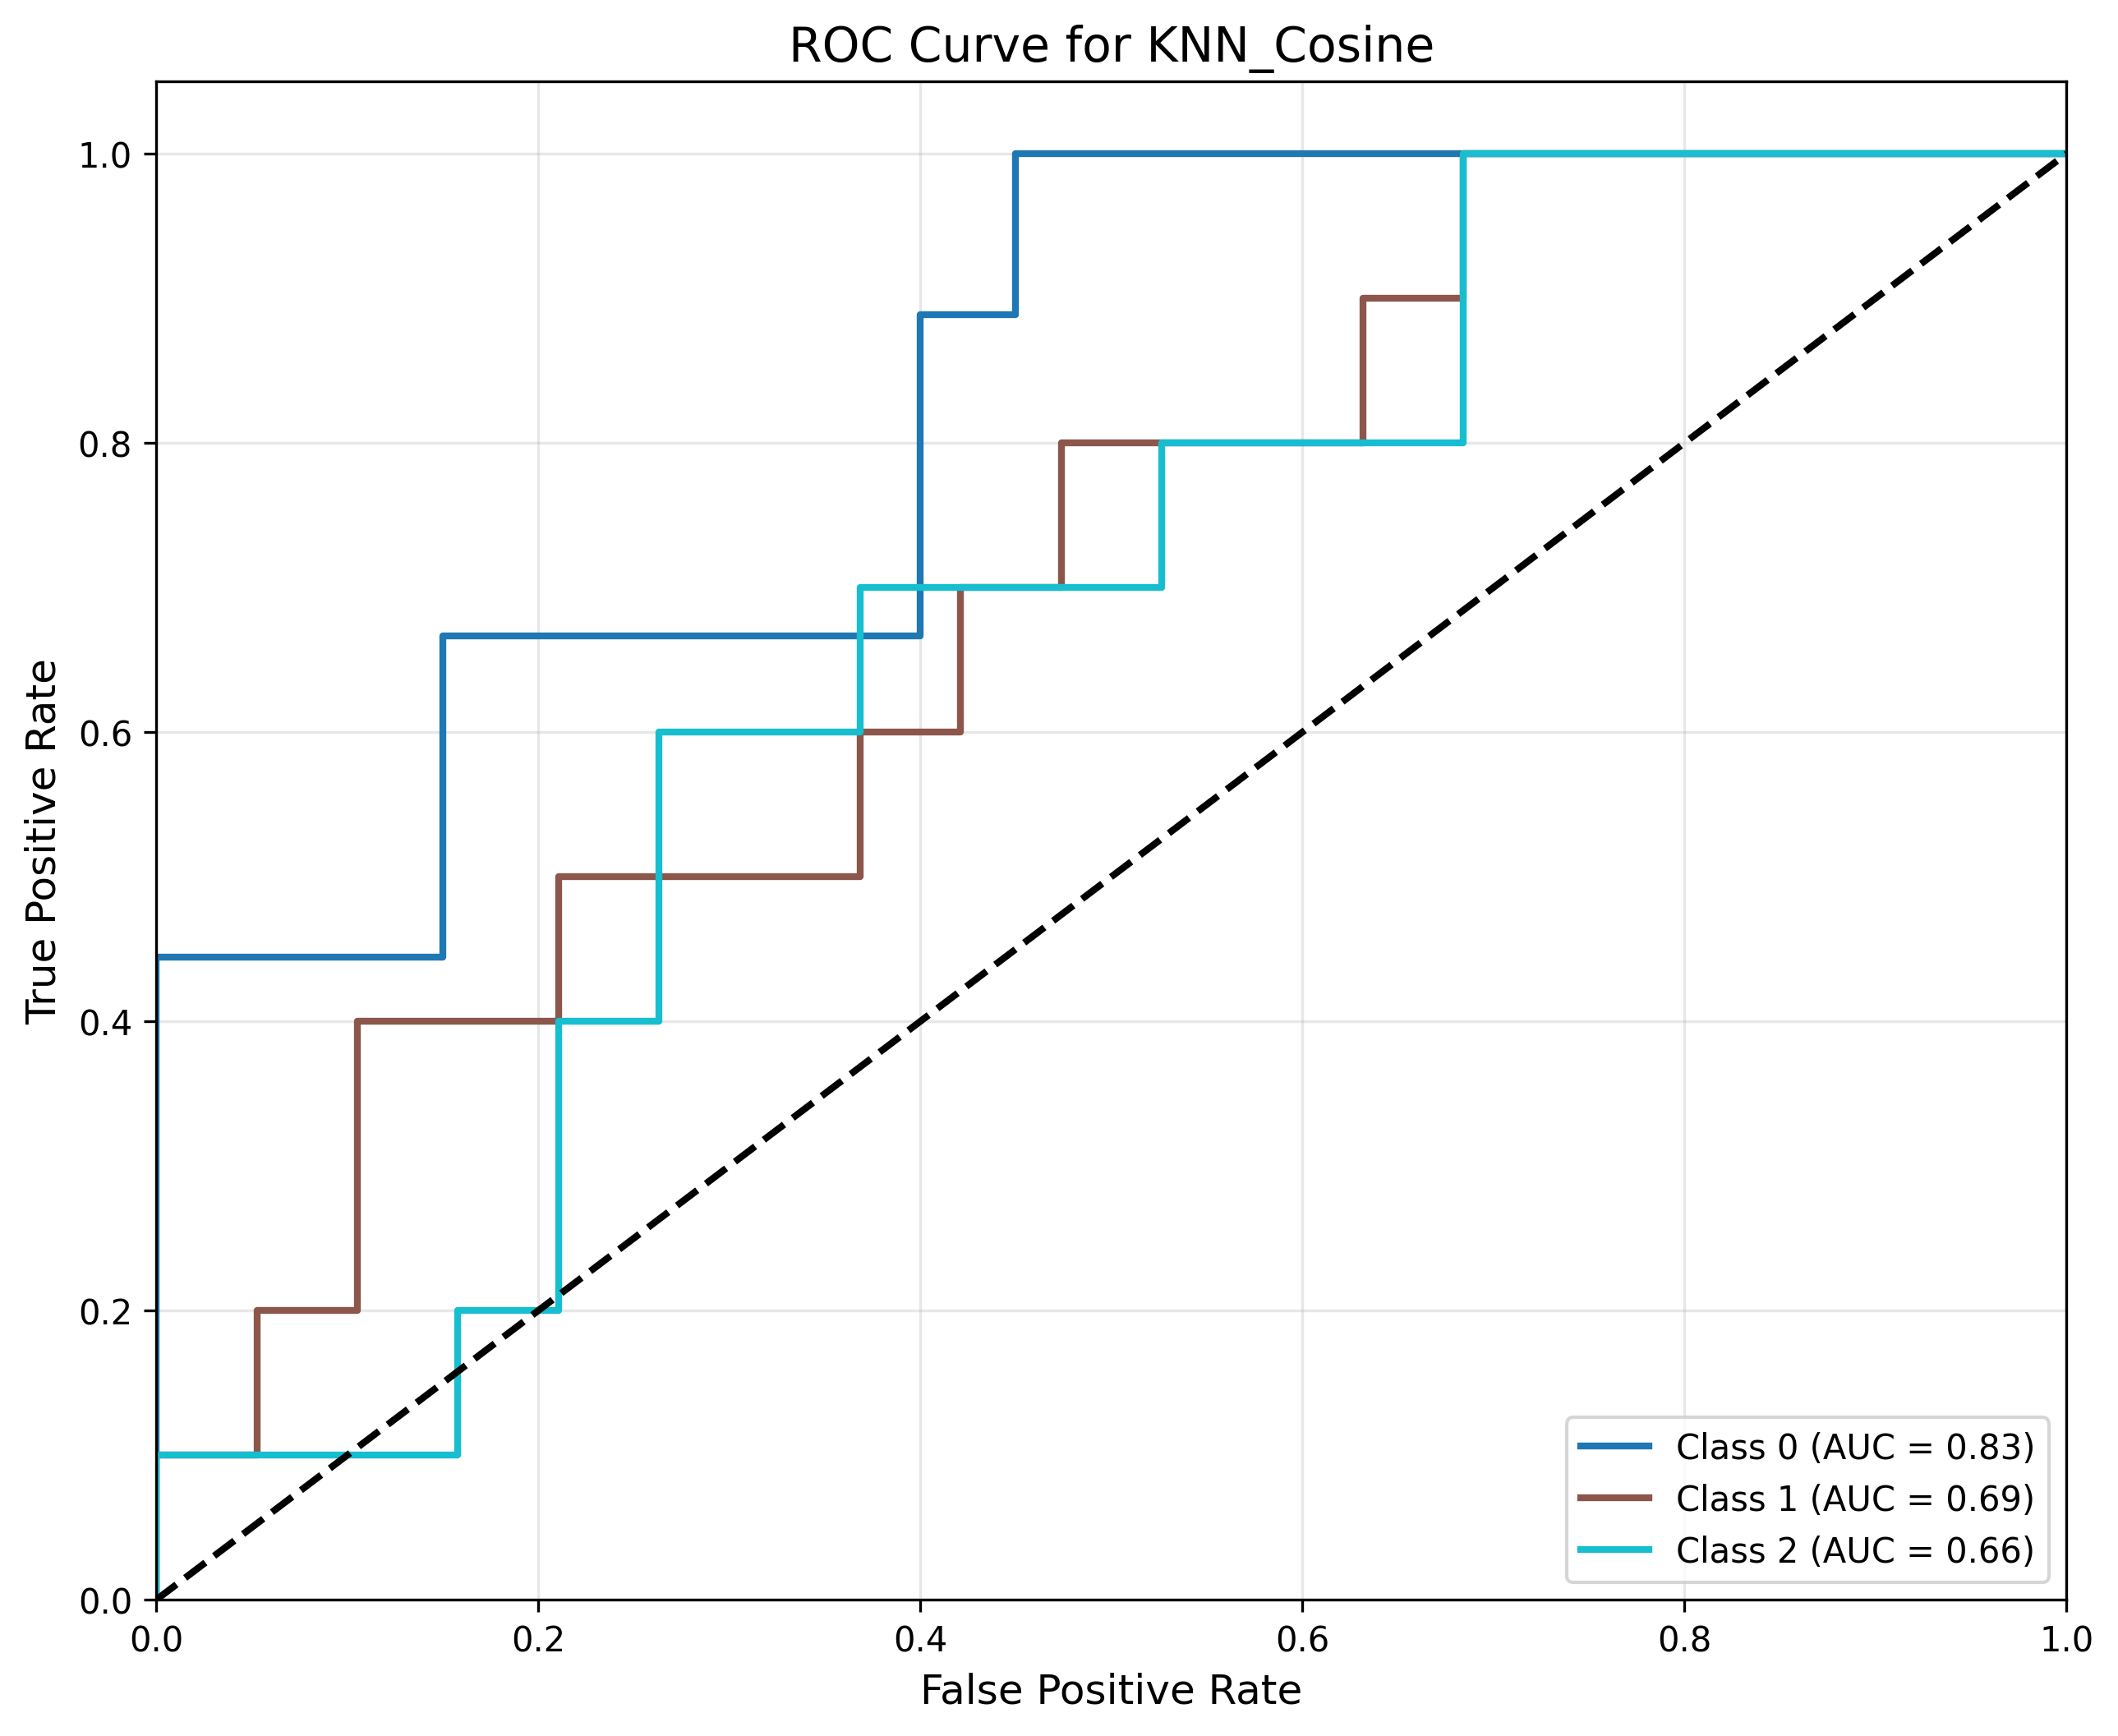
\includegraphics[width=\textwidth]{code/ResultsMainAugZip/plots/Block3_Probabilistic_Experiment_II/roc_curve_KNN_Cosine.png}
            \caption{ROC Curve}
        \end{subfigure}
    \end{figure}
    
    % Block 4: SVM Variants (Experiment II)
    \begin{figure}[!ht]
        \begin{subfigure}{0.5\textwidth}
            \centering
            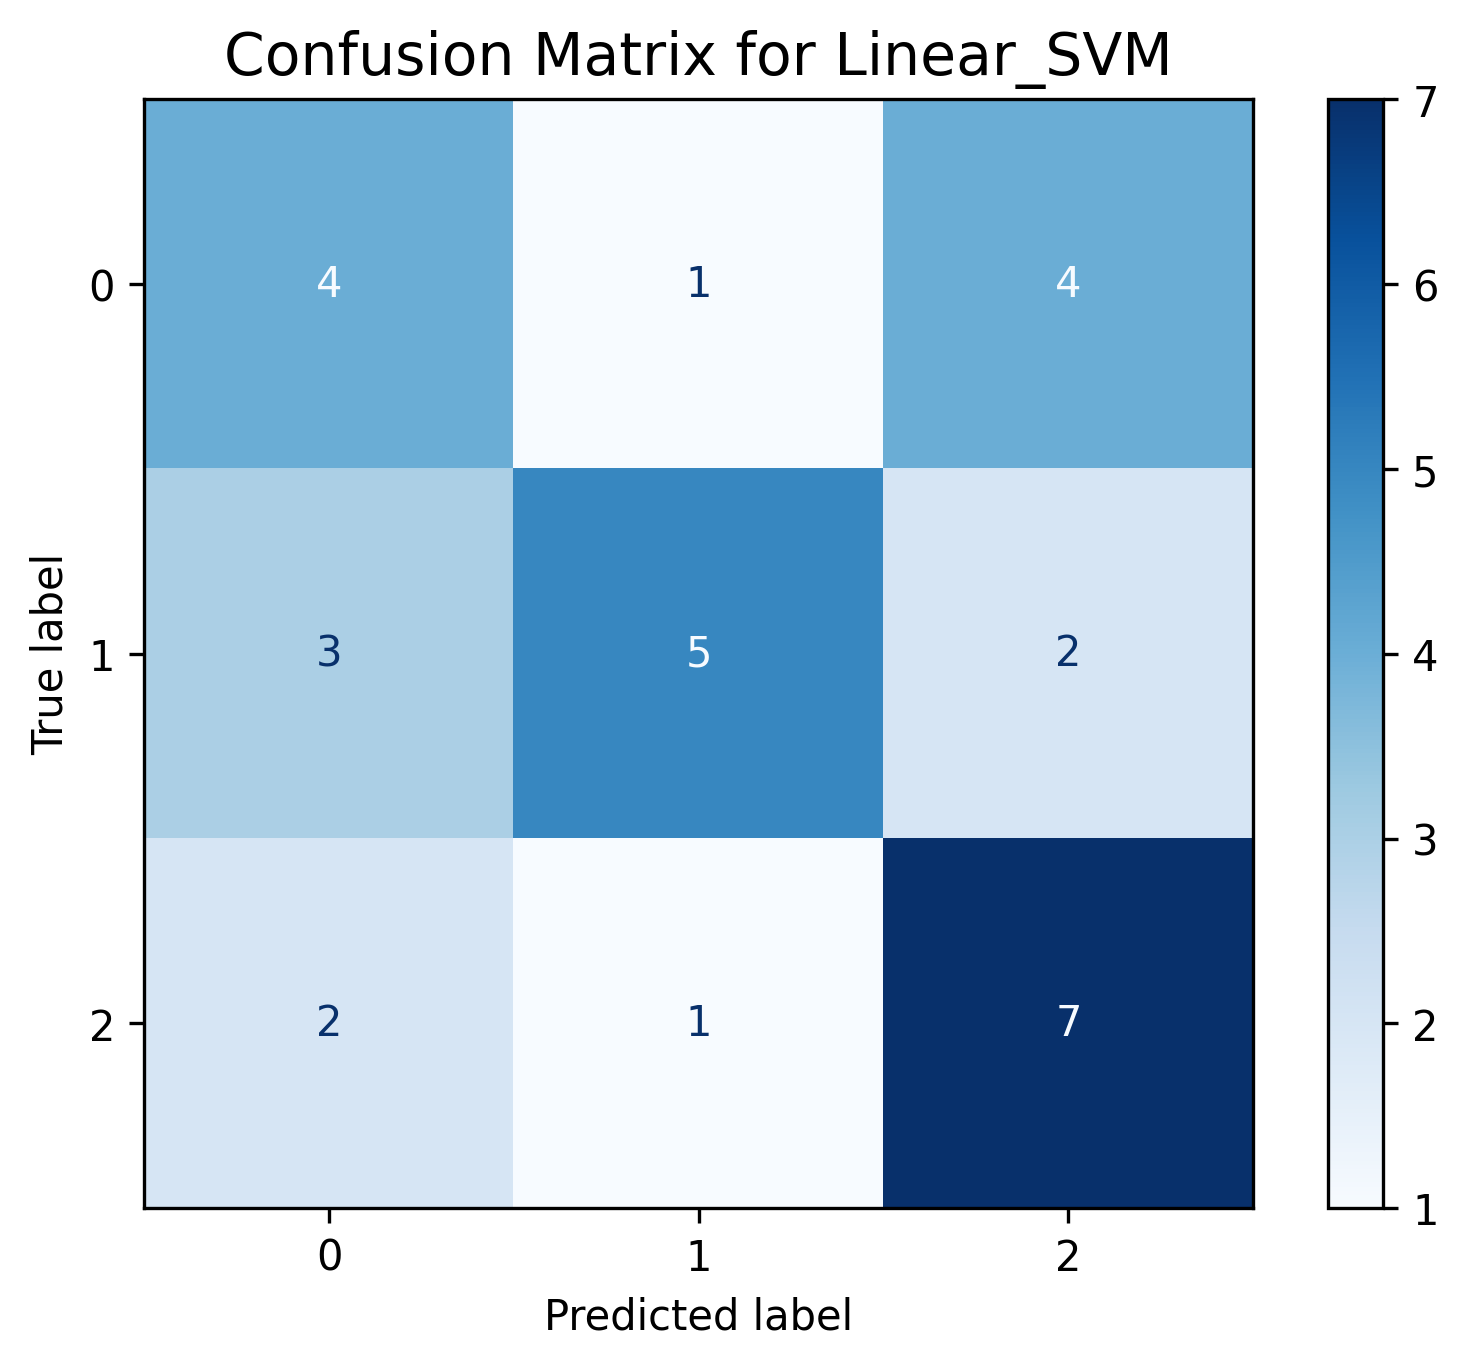
\includegraphics[width=0.9\textwidth]{code/ResultsMainAugZip/plots/Block4_SVM_Variants_Experiment_II/confusion_matrix_Linear_SVM.png}
            \caption{Confusion Matrix}
        \end{subfigure}
        \begin{subfigure}{0.5\textwidth}
            \centering
            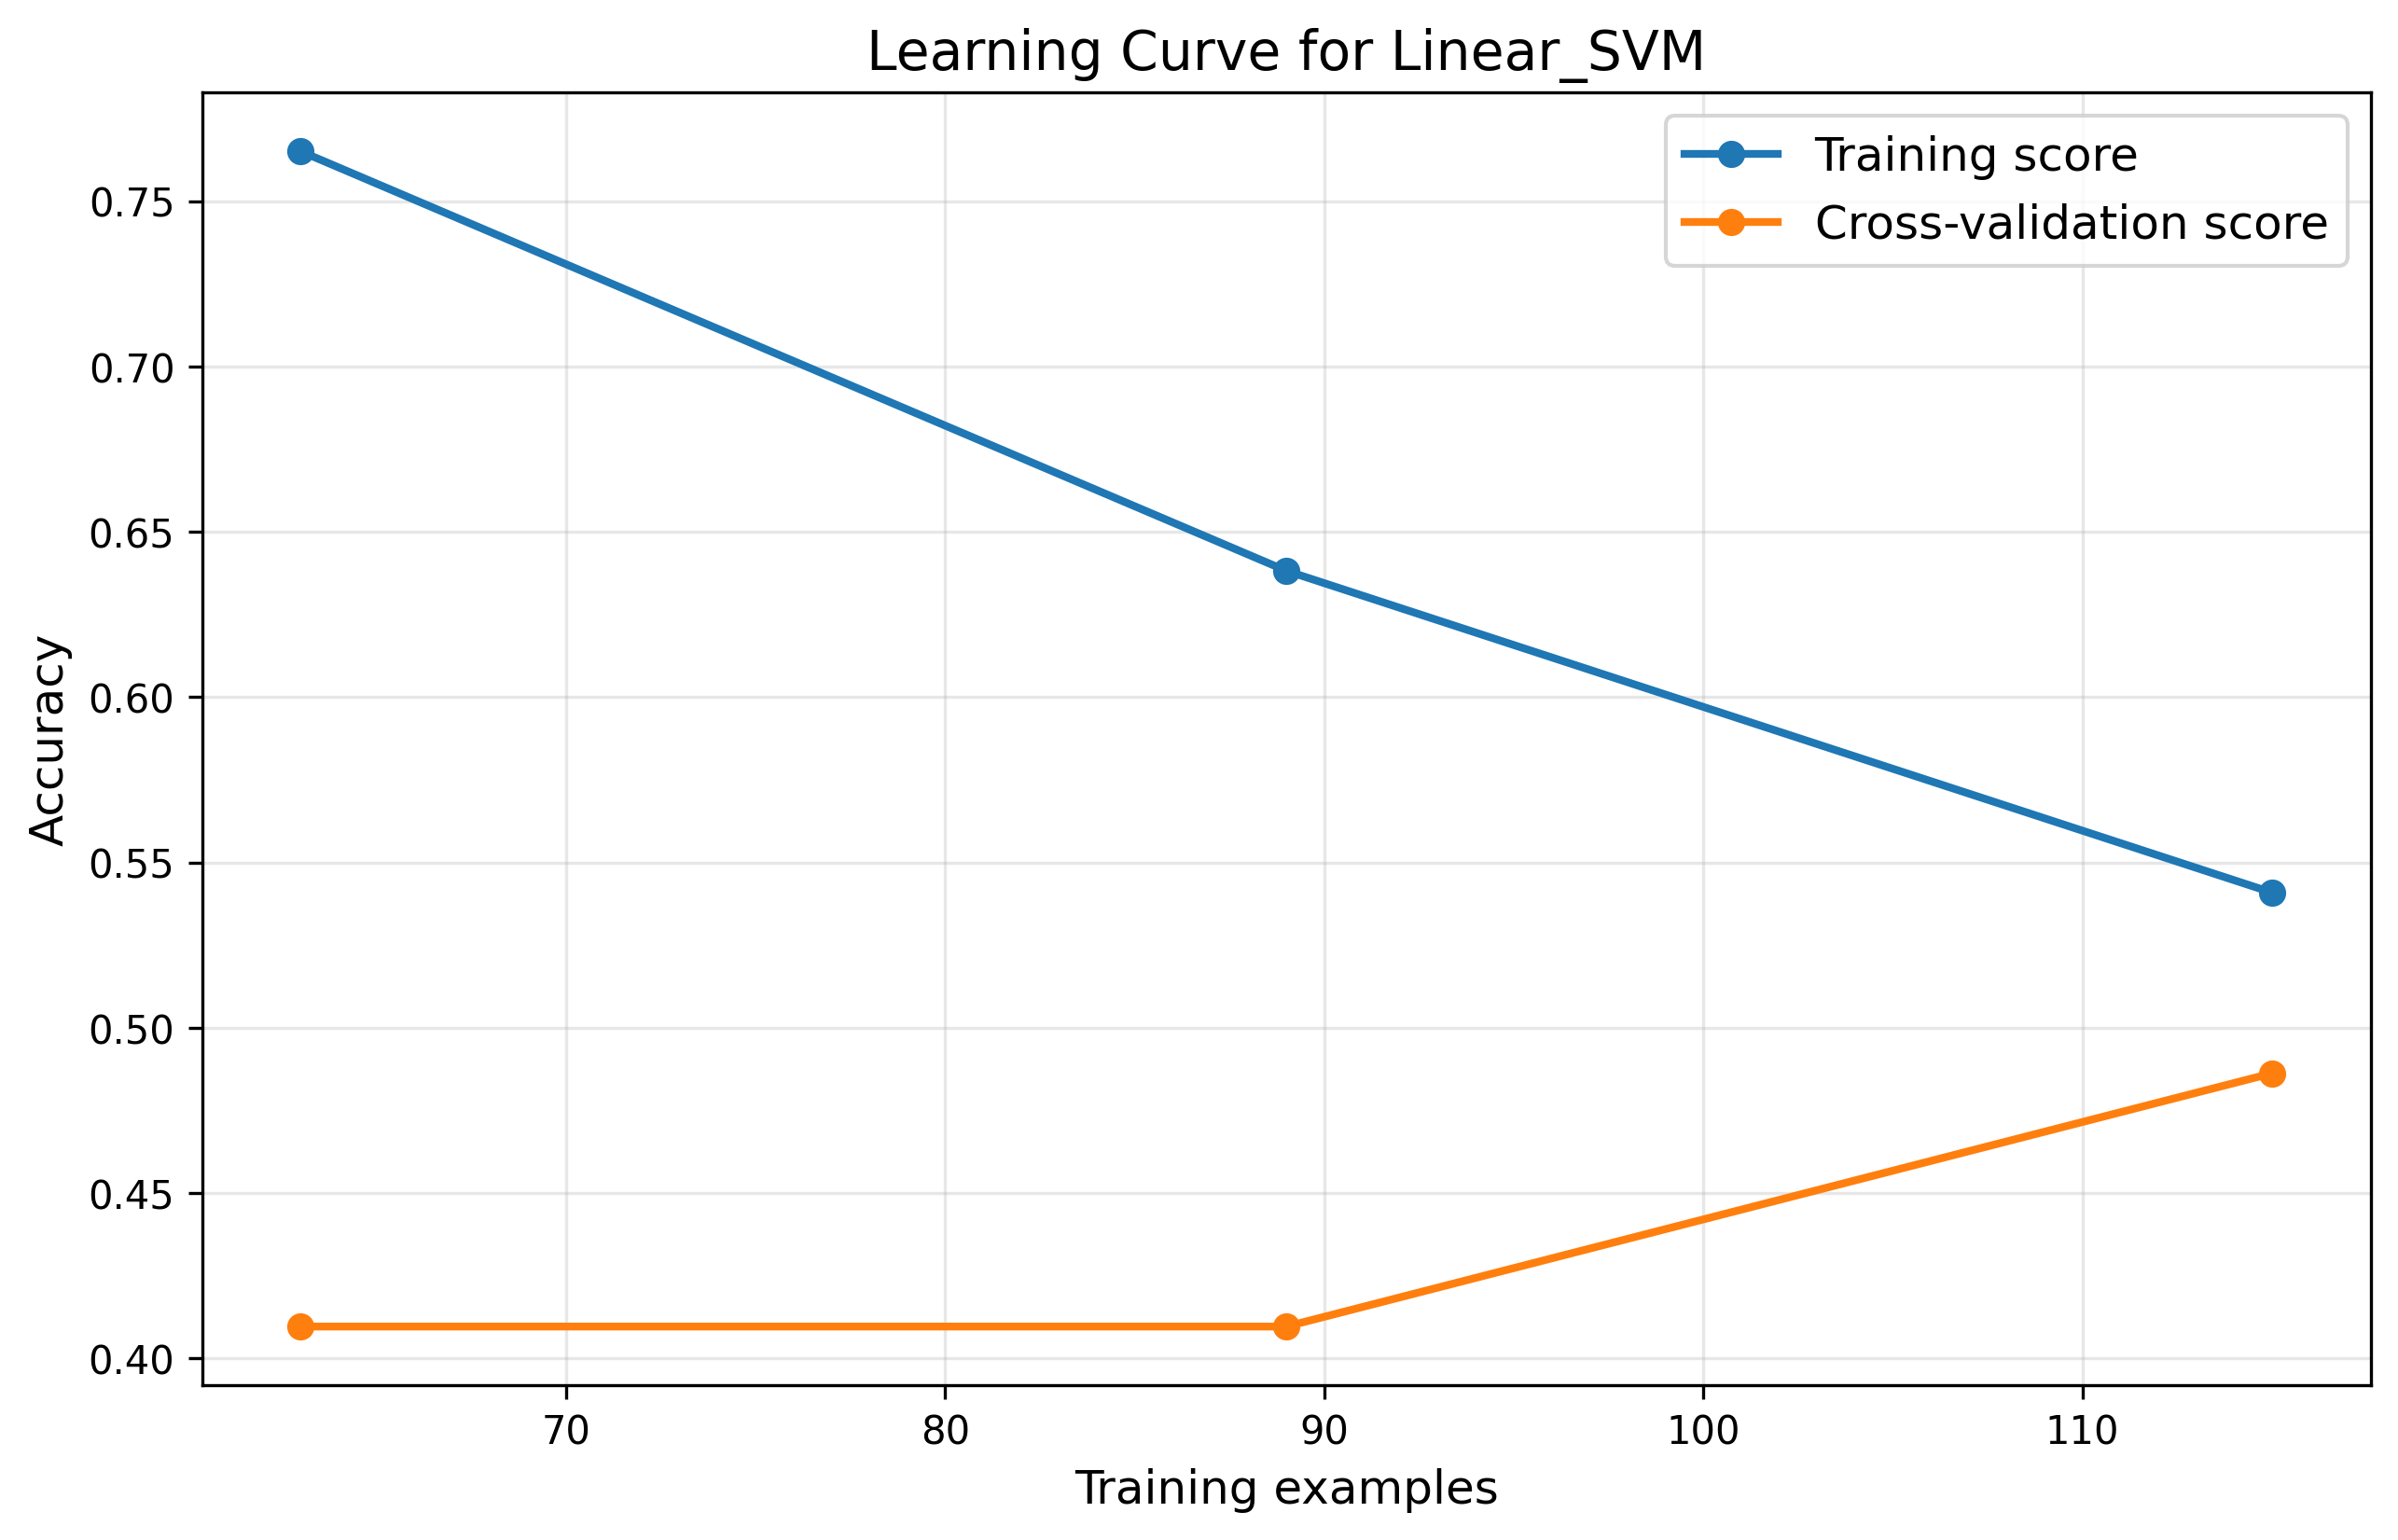
\includegraphics[width=0.9\textwidth]{code/ResultsMainAugZip/plots/Block4_SVM_Variants_Experiment_II/learning_curve_Linear_SVM.png}
            \caption{Learning Curve}
        \end{subfigure}
    \end{figure}

    \newpage

  \section{Discussion}
  
  The results demonstrate significant performance differences between the two experiments. Experiment I, with its larger dataset, 
  achieved substantially higher accuracy (up to 87.34\%) compared to Experiment II (maximum accuracy of 55.17\%). This highlights 
  the importance of dataset size in pattern recognition tasks.
  
  Interestingly, data augmentation did not improve performance in this context, as evidenced by the superior results from 
  Experiment I which did not use augmentation. This suggests that for pressure-based position classification, having a naturally 
  larger and more diverse dataset may be more beneficial than artificially augmenting a smaller dataset.
  
  Among classifiers, KNN variants consistently performed well across both experiments, suggesting their suitability for this 
  type of classification task. SVM variants showed the poorest performance, potentially due to the high dimensionality of 
  the feature space or suboptimal parameter selection.

  \footnote{Sorry, Latex maded a mess with my tables and figures.}

  \section{Conclusions}
  
  This study demonstrates the effectiveness of LBP features combined with KNN classifiers for patient bed position classification. 
  The key findings are:
  
  \begin{enumerate}
    \item Dataset size significantly impacts classification performance, with larger datasets yielding better results
    \item KNN classifiers, particularly KNN Coarse and KNN Medium, achieved the highest accuracy (87.34\%)
    \item Data augmentation through pixel shifting did not improve performance in this application
    \item SVM classifiers underperformed compared to other methods for this specific task
  \end{enumerate}
  
  Future work should explore additional feature extraction methods, deeper neural network architectures, and more sophisticated 
  data augmentation techniques that better preserve the spatial relationships in pressure data.

  \newpage

  \printbibliography

\end{document}
